\documentclass[a4,11pt,dutch,oneside,openany]{book} %twoside for rectoverso
\usepackage[dutch,english]{babel}
\usepackage{float}
\usepackage{epsfig}
\usepackage{amssymb,listings,color,textcomp,marvosym,flafter,longtable,subfigure,amsfonts,rotating}
\usepackage{verbatim}
\usepackage{latexsym}
\usepackage{amsthm}

\usepackage{multirow}
\usepackage{array,pstricks,listings}
\usepackage[vlined,ruled]{algorithm2e}
\usepackage[a4paper,verbose, centering,reversemp]{geometry}
\usepackage[latin1]{inputenc}
\usepackage{fancyhdr}
\usepackage{hhline}     
\usepackage[times]{quotchap}
\usepackage[font={small},labelfont={bf},center]{caption}
\usepackage{times}
\usepackage{wrapfig}
\usepackage{floatflt}
\usepackage{xcolor}
\usepackage{xspace,upgreek}
\usepackage[calcwidth,newparttoc]{titlesec}
\usepackage{titletoc}
\usepackage{listings}
\usepackage{url}
\usepackage{enumitem}
\usepackage{rotating}
\usepackage{pdflscape}
%\usepackage[bottom]{footmisc}
\definecolor{chaptergray}{rgb}{0.85,0.85,0.85}
\parskip=\medskipamount
\usepackage[version=3]{mhchem}
\usepackage[Gray, squaren, thinqspace,thinspace]{SIunits}
\DeclareGraphicsExtensions{jpg,png}
\newcommand{\chpijlr}{\ensuremath{\hspace{1em}\longrightarrow\hspace{1em}}}

\usepackage{setspace}
\setstretch{1.2}

\lstset{
	numbers=left,
	stepnumber=0,    
	firstnumber=1,
	numberfirstline=true
}

\renewcommand{\familydefault}{\sfdefault}


% Cuz arial is not supported? DIG DEEPER!
%\usepackage{helvet}
%\renewcommand{\familydefault}{\sfdefault}

\geometry{bottom=2.4cm,rmargin=2.0cm,lmargin=3.0cm,top=2.5cm} % 10pt op a4

\geometry{marginpar=2.5cm,marginparsep=0cm}

\setlength{\textwidth}{16.5cm}


%%%%%%%%%%%%%%%%%%%%%%%%%%%%%%%%%%%%%%%

%\renewcommand{\topfraction}{0.8}

%%%%%%%%%%%%%%%%%%%%%%%%%%%%%%%%%%%%%%%

%%%%%%%%%%%%%%%%%%%%%%%%%%%%%%%%%%%%%%
%% change for subfigure
\renewcommand{\subfigcapskip}{0pt}
%%%%%%%%%%%%%%%%%%%%%%%%%%%%%%%%%%%%%%

%%%%%%%%%%%%%%%%%%%%%%%%%%%%%%%%%%%%%%%
% headings %

\fancypagestyle{plain}{
	\fancyhf{}
	\renewcommand{\headrulewidth}{0pt}
	\renewcommand{\footrulewidth}{0pt}}

\pagestyle{fancy}
\fancyhf{} %clear all header and footer fields
%\addtolength{\headwidth}{\marginparsep}
%\addtolength{\headwidth}{\marginparwidth}

\renewcommand{\chaptermark}[1]{\markboth{\chaptername\ \thechapter. \ #1}{}}

%\renewcommand{\chaptermark}[1]{\markboth{#1}{}}
%\renewcommand{\sectionmark}[1]{\markright{\thesection\ #1}}

%\newcommand\fdtsvrightmarktmp{{\scshape\small Chapter }}
%\newcommand\fdtsvrightmark{{\scshape\small{Acknowledgment}}}
%\newcommand\fdtsvleftmark{{\scshape\small{Dankwoord}}}

%\newcommand\oddpageleftmark{}
%\newcommand\evenpagerightmark{}

%\fancyhead[LE,RO]{\itshape\bfseries\small\thepage}
%\fancyhead[HL]{\itshape\bfseries\small\leftmark}
%\fancyhead[RE]{\itshape\bfseries\small\rightmark}
%\fancyfoot[FC]{\bfseries\small\thepage}
%\fancyhead[LO]{\oddpageleftmark}
%\fancyhead[RE]{\evenpagerightmark}
%\fancyhead[HL]{\nouppercase{\leftmark}}
%\fancyfoot[C]{\itshape\bfseries\footnotesize \chaptername\ \thechapter}

%%%%%%%%%%%%%%%%%%%%%%%%%%%%%%%%%%%%%%%%%%%%%%%%%%%%


%%%%%%%%%%%%%%%%%%%%%%%%%%%%%%%%%%%%%%%%%%%%%%%%%%%%
% depth of numbering and depth of table of contents %

\setcounter{tocdepth}{3} % titels tot en met niveau subsubsection worden in table of contents opgenomen
\setcounter{secnumdepth}{3} % tot en met niveau subsubsection wordt er genummerd
%%%%%%%%%%%%%%%%%%%%%%%%%%%%%%%%%%%%%%%%%%%%%%%%%%%






%%%%%%%%%%%%%%%%%%%%%%%%%%%%%%%%%%%%%%%%%%%%%%%%%%%%
%%% Nog een paar andere zaken  %%%%
%% om een cross-ref naar een voetnoot te kunnen maken definier ik \usefn %%
%\newcommand{\usefn}[1]{\mbox{\textsuperscript{\normalfont#1}}}
%
%\setlength{\captionindent}{1cm}
%\renewcommand{\captionfont}{\small \itshape \mdseries \rmfamily}
%\renewcommand{\subcapsize}{\footnotesize \itshape \mdseries \rmfamily}
%
%\AtBeginDocument{%
%%   \renewcommand{\figurename}{Fig.}%
%%   \renewcommand{\tablename}{TABLE}%
%   \renewcommand{\tablename}{Table}
%   \renewcommand{\bibname}{References}%
%}

%%%%%%%%%%%%%%%%%%%%%%%%%%%%%%%%%%%%%%%%%%%%%%%%%%%


\renewcommand{\baselinestretch}{1.1}
% space between two paragraphs should be larger than between two lines of text
\newcommand{\npar} {\par \vspace{2.3ex plus 0.3ex minus 0.3ex}} 
% no indentations
\setlength{\parindent}{0cm}
% makes all pages the height of the text on that page, and no extra vertical space is added
\raggedbottom

% define part label
\titleformat{\part}[display]{\flushright\bfseries\vspace{-10cm}} 
{\usefont{OT1}{pag}{b}{n}\fontsize{50}{54}\selectfont{DEEL~\thepart}} {0pt} {\vspace{0.5cm}\huge\usefont{OT1}{pag}{m}{n}\fontsize{25}{30}\selectfont\uppercase} [\thispagestyle{empty}\pagecolor{chaptergray}]
% define chapter label
\titleformat{\chapter}[hang]{\vspace{-3cm}\pagecolor{white}}
{\usefont{OT1}{pag}{b}{n}\fontsize{26}{28}\selectfont {~\thechapter}}{10pt}{\usefont{OT1}{pag}{m}{n}\fontsize{22}{24}\selectfont}[{\thispagestyle{empty}\vspace{2cm}}]
% define section label
\titleformat{\section}[hang]{}
{\usefont{OT1}{pag}{b}{n}\fontsize{14}{16}\selectfont\thesection}{16pt}{\usefont{OT1}{pag}{b}{n}\fontsize{14}{16}\selectfont}[{}\vspace{0.25cm}]

\titleformat{\subsection}[hang]{}
{\usefont{OT1}{pag}{b}{n}\selectfont\thesubsection}{13pt}{\usefont{OT1}{pag}{b}{n}\selectfont}[{}\vspace{0.25cm}]
% define subsubsection label
\titleformat{\subsubsection}[hang]{\sffamily}
{\usefont{OT1}{pag}{m}{n}\fontsize{11}{12}\selectfont\thesubsubsection}{13pt}{\usefont{OT1}{pag}{m}{n}\fontsize{11}{12}\selectfont}[{}\vspace{0.05cm}]
% define paragraph label
\titleformat{\paragraph}[runin]{\sffamily}
{\usefont{OT1}{pag}{b}{n}\selectfont\theparagraph}{}{}[{}]

% define the headers and the footers
\renewcommand{\chaptermark}[1]%
{\markboth{ \MakeUppercase{CHAPTER~\thechapter \mdseries{~~~#1}}}{}}
\renewcommand{\sectionmark}[1]%
{\markright{\fontsize{10}{12} \selectfont\MakeUppercase{\thesection \mdseries{~~~#1}}}}
\renewcommand{\headrulewidth}{0.15pt}
\renewcommand{\footrulewidth}{0pt}
\newcommand{\helv}{%
	\fontfamily{phv}\fontseries{b}\fontsize{8}{10}\selectfont}
\fancyhf{}
\fancyhf[HR]{\helv \fontsize{10}{12} \selectfont \thepage}
\fancyhf[HL]{\helv \fontsize{10}{12} \selectfont \rightmark}
%\fancyhf[HL]{\helv \rightmark}
%\fancyhead[RE]{\helv \rightmark}
\hyphenation{dif-fe-ren-ti-aal-ver-ge-lij-king-en spe-ci-fie-ke
op-los-sing ver-mij-den be-na-de-ring be-na-de-rings-tech-nie-ken
dif-fe-ren-ti-aal-ver-ge-lij-king stap-groot-te me-tho-de stap-groot-te ster-re-tjes
le-vert waar-om toe-pas-sings-ge-bied ver-ge-lij-king-en La-pla-ce-ge-trans-for-meer-de
bij-ge-volg rich-tings-vel-den zelf-werk-zaam-heid ver-ant-woor-de-lijk-heid ge-schre-ven
weer-ge-ge-ven werk-ruim-te im-pli-ciet uit-een-ge-zet voor-ge-steld stij-ve be-schouw-en
men-se-lijke tijds-in-ter-val hier-voor toe-pas-sing be-wer-king-en me-tho-des
tijd-stip-pen ge-ge-ven op-los-sings-in-ter-val i-te-ra-tie-sche-ma ver-wij-de-ren
Tay-lor-ont-wik-ke-ling sta-bi-li-teits-pro-ble-men ver-we-zen-lijk-en stel-sels
stabiliteitsproblemen even-wichts-punt bui-ten-tem-pe-ra-tuur rand-waar-de-pro-bleem
be-gin-waar-de-pro-bleem Taylor-reeks-ont-wikke-ling ont-wik-keld rich-tings-vec-to-ren
vol-doet op-los-sings-me-tho-des ver-wij-zen ver-ge-lijkt bij-ko-men-de uit-ge-voerd
MATLAB struc-tuur-naam struc-tuur-elemen-ten lij-nen hoe-veel-heden wis-kun-di-ge
na-tuur-lij-ke om-ge-ving ver-an-de-ring bij-voor-beeld Toe-pas-sen op-los-sings-do-mein
drie-punts-ope-ra-tor ite-ra-ties be-na-de-rings-sche-ma stijl-op-ties be-we-ging
af-we-zig-heid veel-al ge-lijk-aar-di-ge Wolf-ram mo-del-si-mu-la-tie open-source}


\lstdefinelanguage{JavaScript}{
	keywords={break, case, catch, continue, debugger, default, delete, do, else, false, finally, for, function, if, in, instanceof, new, null, return, switch, this, throw, true, try, typeof, var, void, while, with},
	morecomment=[l]{//},
	morecomment=[s]{/*}{*/},
	morestring=[b]',
	morestring=[b]",
	ndkeywords={class, export, boolean, throw, implements, import, this, get},
	keywordstyle=\color{blue}\bfseries,
	ndkeywordstyle=\color{darkgray}\bfseries,
	identifierstyle=\color{black},
	commentstyle=\color{purple}\ttfamily,
	stringstyle=\color{red}\ttfamily,
	sensitive=true
}

\lstset{
	language=JavaScript,
	backgroundcolor=\color{lightgray},
	extendedchars=true,
	basicstyle=\footnotesize\ttfamily,
	showstringspaces=false,
	showspaces=false,
	numbers=left,
	numberstyle=\footnotesize,
	numbersep=9pt,
	tabsize=2,
	breaklines=true,
	showtabs=false,
	captionpos=b
}

\lstset{language=JavaScript,keywordstyle={\bfseries \color{red}}}

\begin{document}
\sloppy
%language=Matlab,commentstyle=
\selectlanguage{dutch}
\definecolor{licht-grijs}{gray}{0.95}
\lstset{language=Matlab, framexleftmargin=5mm,belowcaptionskip=5mm,
frame=none,basicstyle={\ttfamily\small},
stringstyle=\small,commentstyle=\textcolor[rgb]{0.53,0.53,0.53},
backgroundcolor=\color{licht-grijs},showspaces=false,framexleftmargin=-2pt,showstringspaces=false,upquote=true}

\frontmatter

%  Titelblad

\begin{titlepage}

\fontsize{12pt}{14pt}

\begin{center}

% Het logo van de Universiteit Gent

\includegraphics[height=3cm]{Figuren/odisee_logo.jpg}

\vspace{1cm}

\fontsize{14pt}{17pt}\selectfont
\textsc{Elektronica-ICT}
\fontsize{12pt}{14pt}\selectfont
\vspace{0.3cm}

\vspace{1cm}

Academiejaar 2016--2017

\vspace{5.8cm}

\fontsize{17.28pt}{21pt}\selectfont

% De titel van bachelorproef:
\textsc{Dynamisch annoteren van afbeeldingen in CX Social}

\fontseries{m}
\fontsize{14pt}{16pt}\selectfont

\vspace{5.8cm}

% De auteur:
\textbf{Gheerwijn Clicque}

\vspace{1.0cm}
\fontseries{m}
\fontsize{12pt}{14pt}\selectfont

% De promotor:
Promotor: Jurriaan Persyn\\ 
Mentor: Davy De Winne

\vspace{2cm}

\end{center}
\end{titlepage}

\thispagestyle{empty}

%\iffalse
\rule[-0.4\baselineskip]{0cm}{10\baselineskip}   
\par \vspace{2.3ex plus 0.3ex minus 0.3ex}
De auteurs en promotoren geven de toelating deze scriptie voor consultatie beschikbaar te stellen en delen ervan te kopi�ren voor persoonlijk gebruik. Elk ander gebruik valt onder de beperkingen van het auteursrecht, in het bijzonder met betrekking tot de verplichting uitdrukkelijk de bron te vermelden bij het aanhalen van resultaten uit deze scriptie.
\par \vspace{2.3ex plus 0.3ex minus 0.3ex}
The authors and supervisors give the permission to use this thesis for consultation and to copy parts of it for personal use. Every other use is subject to the copyright laws, more specifically the source must be extensively specified when using from this thesis.
\par \vspace{2.3ex plus 0.3ex minus 0.3ex}
%Gent, juni 2015

\vspace{3cm}
%De promotoren, \\

\vspace{2cm}
%\\De auteurs,\\
Gheerwijn Clicque
\thispagestyle{empty} 
\fi


\chapter{Samenvatting}
\vspace{-3cm}
Anno 2017 is sociale media niet meer weg te denken uit ons dagelijks leven. Van presidenten tot dieren, iedereen heeft een wel een profiel op een of andere sociale media platform. CX Social is de customer care tool voor sociale media waar ik van februari 2017 tot mei 2017 een profile manager uitwerkte. Enkele features die CX Social aan hun klanten aanbieden zijn: een gecentraliseerde inbox,  een dashboard en een overzichtspagina van de statistieken per profiel. Zo kunnen bedrijven hun klanten zo snel en effici\"{e}nt mogelijk bijstaan. Net zoals alle andere features in de web applicatie van CX Social, moet de profile manager klanten helpen bij het beheren van hun sociale media profielen. Het doel is om een gemeenschappelijke plaats te hebben waar klanten de profiel- en omslagfoto van hun profielen kunnen beheren.

Naast het selecteren van afbeeldingen moeten gebruikers in staat zijn om annotaties toe te voegen aan de omslagfoto. Dit houdt in dat zowel tekst als specifieke prestatie-indicatoren op een afbeelding geplaatst kunnen worden. Met behulp van deze indicatoren kan gemakkelijk informatie aan klanten meegedeeld worden. Mogelijke indicatoren zijn cijfers die aanduiden hoe lang het gemiddeld duurt voor vragen beantwoord worden of hoeveel gebruikers het bedrijf al geholpen heeft de voorbije week. Hoewel dit op het eerste gezicht geen belangrijke informatie voorstelt, valt de invloed hiervan niet te onderschatten. Klanten die op de Facebookpagina van een bedrijf kunnen aflezen dat ze gemiddeld binnen de 10 minuten geholpen worden, zullen eerder een conversatie aangaan dan wanneer ze dit helemaal niet weten.

Beide foto's samen vormen een thema dat ingesteld kan worden op \'{e}\'{e}n of meerdere sociale media profielen. Het instellen zelf gebeurt door het selecteren van de periode wanneer een specifiek thema actief moet zijn op een profiel. Een gebruiker kan kiezen tussen reeds ingestelde business hours (bv. maandag van 9u tot 18u) of een andere periode (bv. van november tot eind december). Zo kunnen thema's ingesteld worden om de foto's aan te passen wanneer een bedrijf open is of wanneer de kerstperiode aanbreekt. 

Na onderzoek naar verschillende bibliotheken die het mogelijk maken om tekst op afbeeldingen te plaatsen, blijkt de Fabric.js bibliotheek de beste oplossing. Met behulp van React worden verschillende componenten aangemaakt om afbeeldingen te annoteren, thema's aan te maken en toe te passen op een profiel. Ook wordt een Node.js service opgesteld die, wanneer nodig, de omslagfoto's zal genereren met aangepaste prestatie-indicatoren om deze uiteindelijk te uploaden naar Facebook of Twitter. 

Uiteindelijk werd succesvol een profile manager ge\"{i}mplementeerd waarmee gebruikers op een eenvoudige manier de omslag- en profielfoto's van hun profielen kunnen beheren. 

\newpage
\chapter{Woord vooraf}
\vspace{-3cm}
Om mijn studies Elektronica-ICT, afstudeerrichting Web \& Mobile Development af te sluiten, kreeg ik de kans om stage te lopen bij Engagor. Uit de toegewezen stageopdracht vloeide ook deze bachelorproef voort. Tijdens de stage maakte ik niet enkel kennis met nieuwe technische zaken zoals frameworks en bibliotheken maar leerde ik ook functioneren in een echte werkomgeving. Ook tijdens het schrijven van deze bachelorproef werd kennis gemaakt met nieuwe technologie\"{e}n en werden nieuwe inzichten verworven. 

Het vlotte en zeer aangename verloop van mijn stage heb ik aan het volledige CX Social team te danken. Graag bedank ik nog dhr. Jurriaan Persyn voor de kans om mijn stage bij Engagor te lopen en dhr. Davy De Winne voor het bijsturen van mijn bachelorproef waar nodig. Ook bedank ik graag dhr. Hans Ott en dhr. Anthony Meirlaen voor alle hulp tijdens de stage en het nalezen van dit werk. 







\iffalse
\begin{slshape}
Met deze bachelorproef willen we onze bacheloropleiding in de Bio-ingenieurswetenschappen afsluiten. Na veel opzoekingswerk zijn we trots op het resultaat. Dit project heeft ons namelijk op verschillende vlakken veel bijgeleerd: het gebruik van de computers in de voeding, programmeren in R, informatie bundelen in een beperkt aantal pagina's, etc.

Uiteraard was dit alles niet mogelijk geweest zonder de hulp van een aantal mensen. We willen dan ook Marlies en Michiel bedanken voor de vele meetings, de tijd die ze voor ons hebben vrijgemaakt en de hulp bij het implementeren van het Naive Bayes algoritme. Zonder hun raad en tips was dit alles ons niet gelukt. Vervolgens gaat onze dank ook uit naar professor De Baets en professor Waegeman voor hun advies bij het schrijven van deze bachelorproef.
\end{slshape}
\fi





\tableofcontents


\chapter{Lijst met gebruikte afkortingen}

\setlist[itemize]{leftmargin=*}
\begin{itemize}
\item[] \textbf{CEM} \qquad Customer Experience Management
\item[] \textbf{CX} \qquad Consumer Experience
\item[] \textbf{KPI} \qquad Key Performance Indicator
\item[] \textbf{PHP} \qquad Hypertext Preprocessor
\item[] \textbf{MySQL} \qquad My Structured Query Language
\item[] \textbf{HTML} \qquad HyperText Markup Language
\item[] \textbf{SVG} \qquad Scalable Vector Graphics
\item[] \textbf{URL} \qquad Uniform Resource Locator
\item[] \textbf{JPEG} \qquad Joint Photographic Experts Group
\item[] \textbf{PNG} \qquad Portable Network Graphics
\item[] \textbf{RGBA} \qquad Red, Green, Blue, Alpha
\item[] \textbf{HSV/HSL} \qquad Hue, Saturation \& Value/Hue, Saturation \& Luminosity
\item[] \textbf{JSON} \qquad JavaScript Object Notation
\item[] \textbf{DOM} \qquad Document Object Model
\item[] \textbf{URI} \qquad Uniform Resource Identifier
\item[] \textbf{AJAX} \qquad Asynchronous JavaScript and XML
\item[] \textbf{ID} \qquad Identity Document
\item[] \textbf{CSRF} \qquad Cross-site request forgery
\item[] \textbf{HTTP} \qquad Hypertext Transfer Protocol
\item[] \textbf{NPM} \qquad Node Package Manager
\end{itemize}	





\mainmatter

%\newacronym{cem}{CEM}{Customer Experience Management}
%\newacronym{cx}{CX}{Consumer Experience}
%\newacronym{kpi}{KPI}{Key Performance Indicator}


%\gls{ny} and \gls{la} are in \gls{us}. 
%\printglossary[type=\acronymtype,title=Lijst met gebruikte afkortingen]
% !TeX spellcheck = <none>
\chapter{Voorstelling van het stagebedrijf}
\vspace{-3cm}
\section{Ontstaan en geschiedenis}

Engagor werd opgericht in 2011 door Folke Lemaitre (ex-werknemer van Netlog) met de bedoeling interactie met klanten, via sociale media, te vereenvoudigen. Sinds 2015 maakt Engagor deel uit van Clarabridge. Dit Amerikaanse bedrijf ontwikkelt software om automatisch online data te verzamelen, te categoriseren en te rapporteren. Gebruikelijk is dit data verkregen van sociale media zoals Facebook en Twitter. Maar andere platformen zoals YouTube, Instagram, Vimeo en Tumbler kunnen ook beheerd worden. Kort samengevat zijn ze dus gespecialiseerd in software voor Customer Experience Management (CEM). Het gaat hier dus vooral om feedback over interacties die plaatsvinden tussen de klanten en het bedrijf. Zo kunnen bedrijven hun strategie aanpassen om hun klanten zo goed mogelijk van dienst te zijn \cite{bp1}. Tegenwoordig is sociale media niet meer weg te denken uit het dagelijkse leven, noch bij particulieren noch bij bedrijven. Dit resulteert in een zeer groot klantenbestand met grote klanten zoals Telenet, NMBS, AirBnb, Ikea, Turkish Airlines, \ldots 

Na de overname werd Engagor onderdeel van CX Social (CX staat hier voor Consumer Experience) \ref{fig:CXSocialLogo}, een van de vier producten van Clarabridge. De andere drie zijn CX Survey, CX Studio en CX Designer. Met CX Survey kunnen surveys aangemaakt en verwerkt worden. De verwerking van surveys gebeurt onder andere met behulp van tekst en sentiment analyse. CX Studio is een \textit{dashboarding tool} waarmee gebruikers hun CEM proces kunnen stroomlijnen. Als laatste is er ook nog CX Designer dat voor data modelering gebruikt wordt \cite{Clarabridge.com}. 

Clarabridge heeft momenteel ongeveer 250 werknemers, verspreid over de hele wereld. Het hoofdkantoor bevindt zich in Reston, Virginia, Amerika. Maar er zijn kantoren in Gent, Larkspur (California), Londen, Barcelona en Singapore \cite{ClarabridgeOffices}. Op elk van deze locaties en in India zijn \textit{support teams} aanwezig. Zo kunnen ze 24/5 en in sommige gevallen zelfs 24/7, hun klanten bijstaan.

Voor mijn stage werk ik aan CX Social. Dit is dus de \textit{customer care tool} voor sociale media. Gebruikers kunnen via de web applicatie snel en gemakkelijk antwoorden op vragen en/of klachten op hun sociale profielen zoals Facebook, Twitter en Instagram. Dit is voor grote bedrijven natuurlijk zeer handig aangezien zij dagelijks gigantisch veel berichten (zowel priv\'{e}berichten als \textit{posts}) op hun profielen moeten verwerken. \'{E}\'{e}n gemeenschappelijke plaats waaruit alle profielen kunnen onderhouden worden, is dus onontbeerlijk. 

\begin{figure}[H]
	\centering
	
\includegraphics[width=0.6\textwidth]{Figuren/CXSocialLogo.png}
	\caption{CX Social Logo \cite{CXSOcialLogo}} 
	\label{fig:CXSocialLogo}
\end{figure} 

Het CXSocial team bestaat uit ongeveer 35 werknemers. Zij werken constant aan het verbeteren en onderhouden van deze \textit{tool}.  Binnen het team werken de meesten als \textit{Full stack software engineer}. Zij werken dus zowel aan de backend van de web applicatie als aan de API en frontend. Het team wordt vervolledigd door mensen die zich bezighouden met \textit{data science} en design. \textit{Data scientists} werken onder andere met \textit{machine learning} en statistieken. Het belang hiervan valt in een sociale media \textit{monitoring tool} niet te onderschatten. Ook het design is zeer belangrijk tijdens het ontwikkelen van een web applicatie. Telkens een nieuw \textit{feature} toegevoegd wordt, wordt hiervan een ontwerp gemaakt om dit nieuwe stukje zo goed mogelijk in het geheel te implementeren. De designers moeten er natuurlijk ook voor zorgen dat hun ontwerpen overeenkomen met alle producten die Clarabridge aanbiedt. Ook moet alles wat ze ontwerpen zo gebruiksvriendelijk mogelijk gemaakt worden \cite{EngagorTeam}. 

Wanneer nieuwe \textit{features} ge\"{i}mplementeerd moeten worden, wordt dit ofwel door \'{e}\'{e}n iemand uitgewerkt of door enkele personen uit het team. Tijdens het ontwikkelen kan feedback en hulp van collega`s ingeroepen worden waardoor iedereen altijd betrokken is bij verschillende projecten. Dit zorgt er voor dat niet enkel degene die het project toegewezen krijgt, weet hoe alles in elkaar zit. Zo is iedereen op elk moment op de hoogte van veranderingen aan de \textit{code base}. 

Op Figuur~\ref{fig:Organigram} is de organisatie binnen het CX Social team te zien. Dit organigram is niet volledig accuraat want de positie van Solutions Engineer moet hier nog aan toegevoegd worden maar het schept een zeer goed beeld van de verschillende functies binnen CX Social. 

\begin{figure}[H]
	\centering
	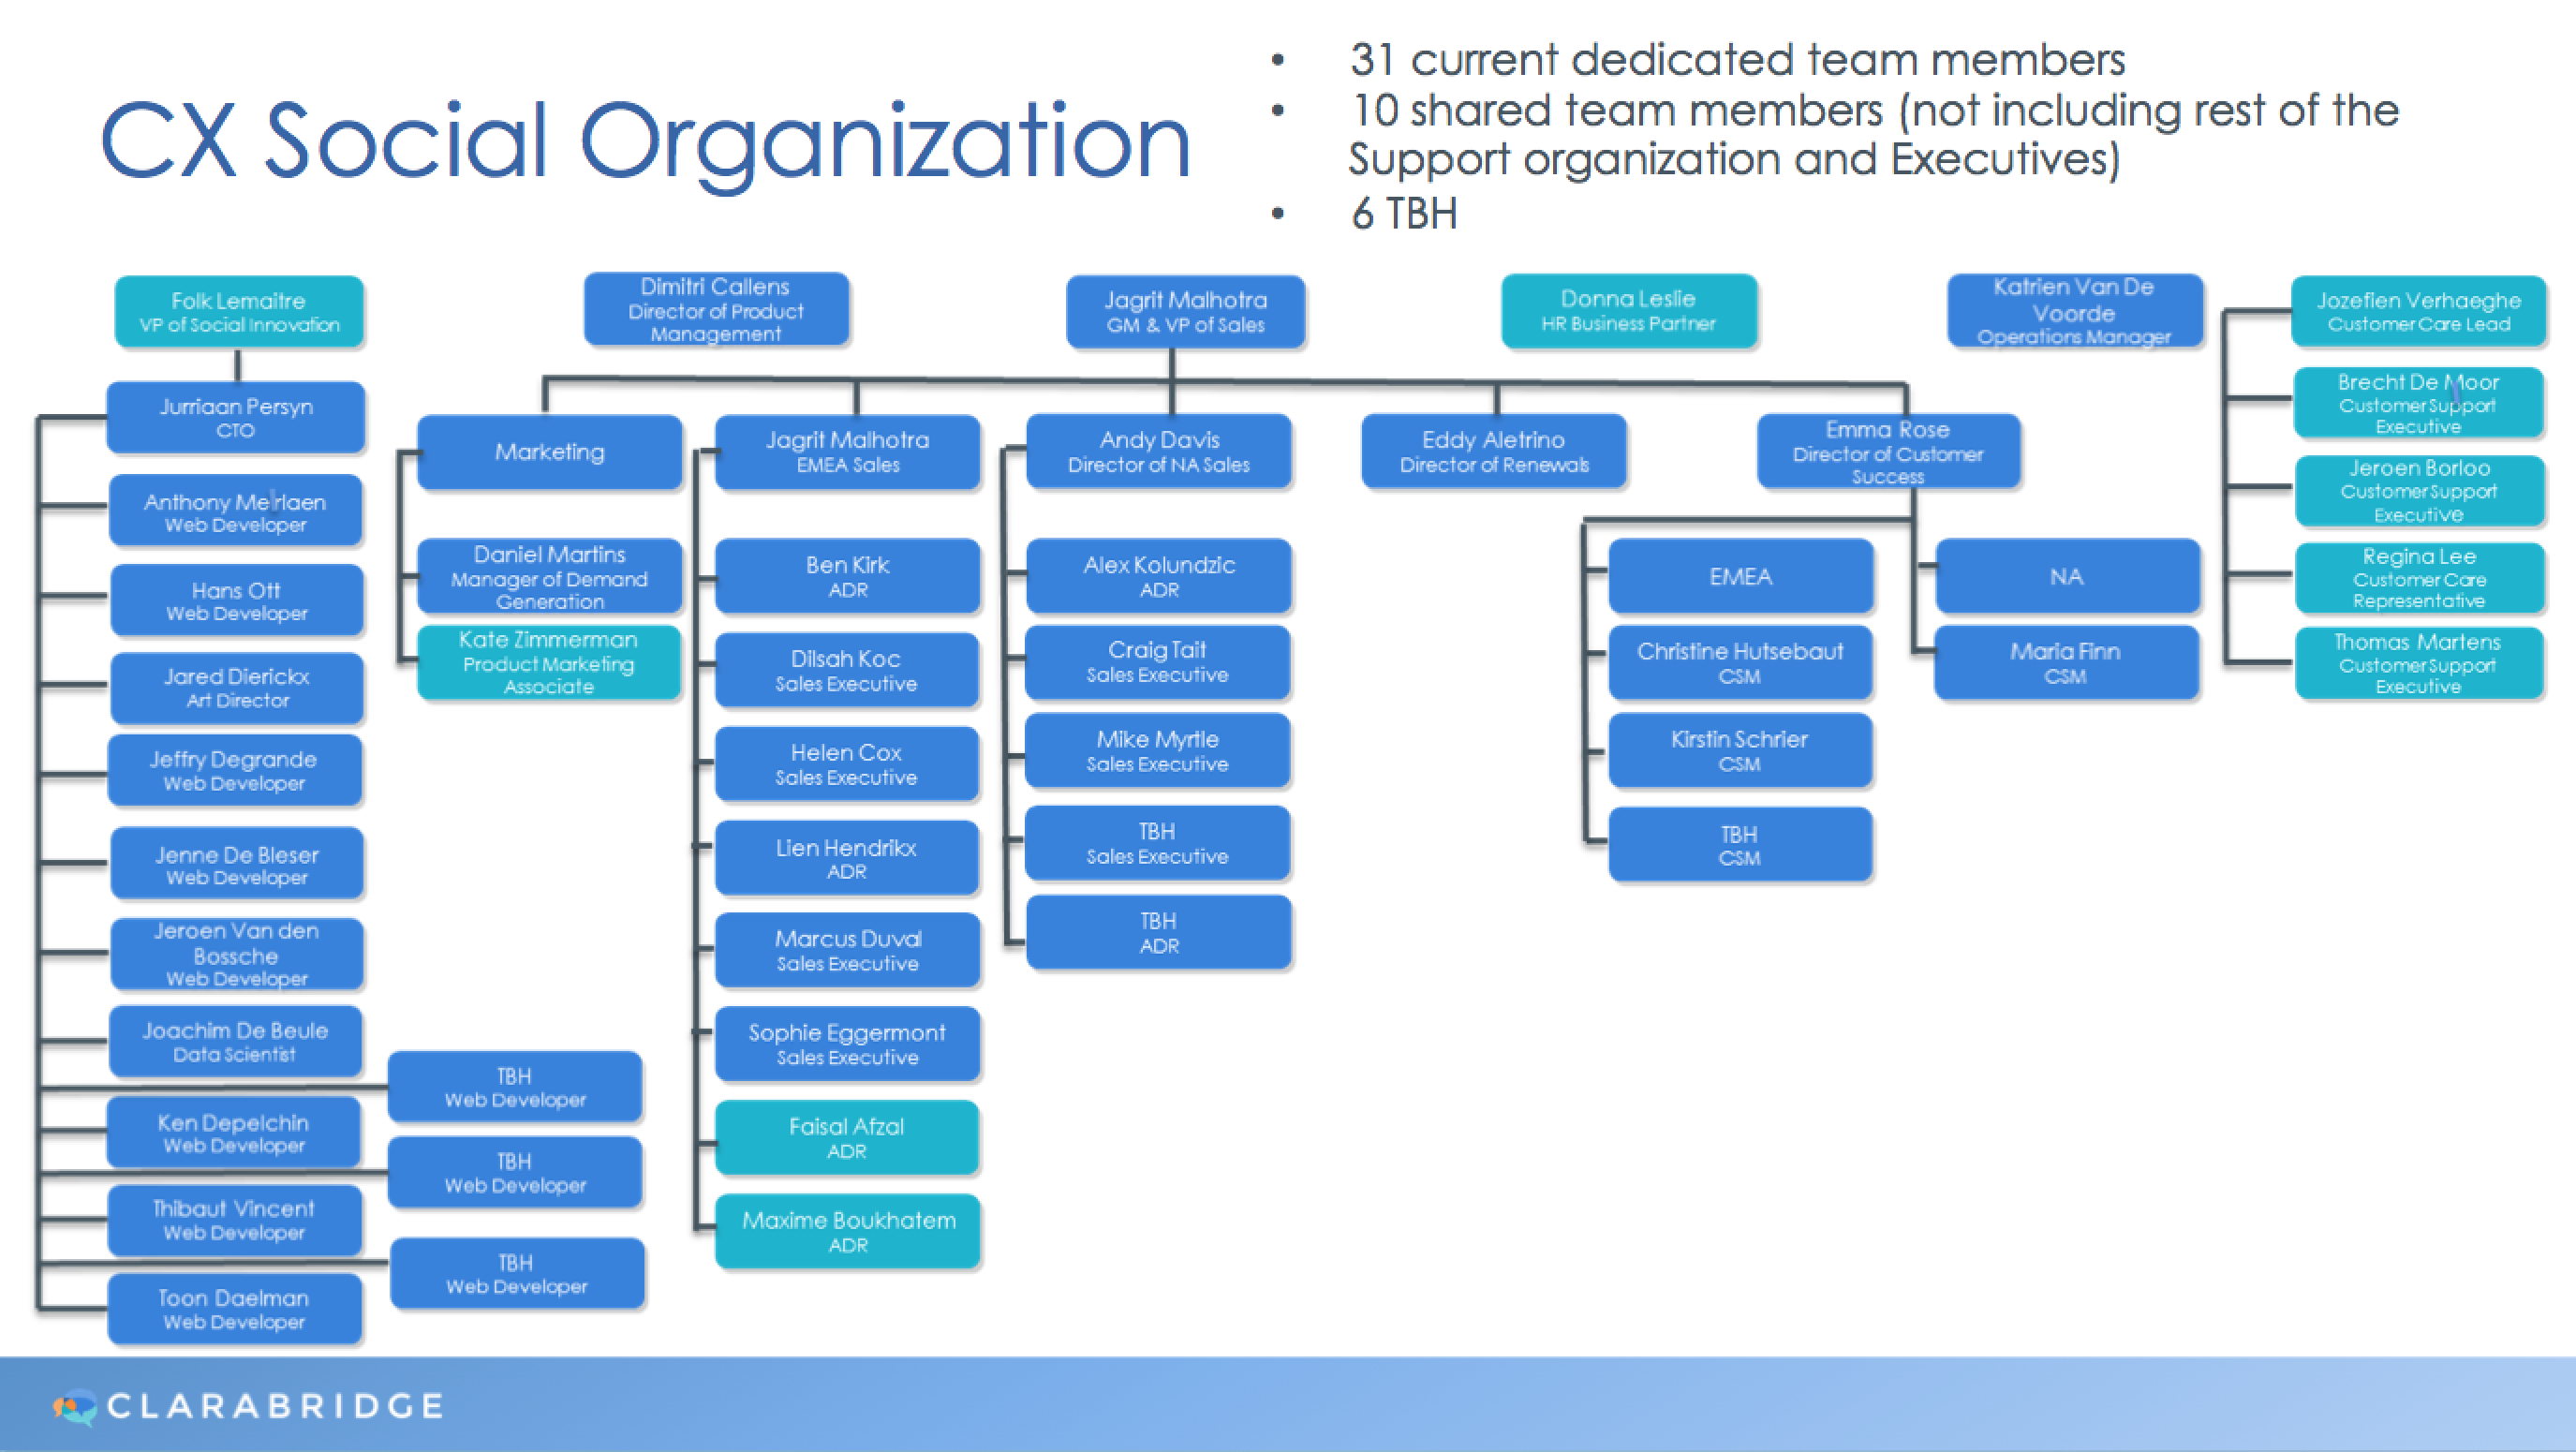
\includegraphics[width=1\textwidth]{Figuren/Organigram.png}
	\caption{Organigram CX Social} %\cite{Pouladzadeh}
	\label{fig:Organigram}
\end{figure} 

\section{CX Social} \label{CXSocial}
Elk product, aangeboden door Clarabridge, is toegespitst op de analyse van customer feedback. CX Social is de sociale media \textit{monitoring}, management en analyse tool die gebruikt wordt door verschillende grote bedrijven om hun klanten beter te ondersteunen. Het principe van de \textit{tool} is dat op \'{e}\'{e}n gemeenschappelijke plaats verschillende profielen beheerd kunnen worden. Zo kunnen onder meer berichten van klanten beantwoord worden, statistieken bekeken worden of kan de inhoud van de profielen aangepast worden. 

Engagor maakt in hun webapplicatie gebruik van PHP, JavaScript, HTML en CSS. Het grootste deel is geschreven in PHP met het DooPHP \textit{framework}. Dit \textit{framework} is momenteel niet meer in ontwikkeling maar werd aangepast voor gebruik binnen de Engagor webapplicatie waardoor verdere ontwikkeling van DooPHP door de ontwikkelaars niet onmiddellijk nodig is \cite{DooPHP}. %Naast PHP en JavaScript frameworks wordt ook gebruik gemaakt van MySQL, Redis, memcached, ElasticSearch en RabbitMQ. 

In de frontend wordt vooral gebruik gemaakt van React (ook gekend als React.js/ReactJS). Dit is een open-source JavaScript bibliotheek, ontwikkeld door Facebook, waarmee zeer gemakkelijk gebruikers interfaces aangemaakt kunnen worden. Met React kunnen componenten gecre\"{e}erd worden, waarin wordt vastgelegd wat gerenderd moet worden voor de gebruiker. React zal ervoor zorgen dat de componenten effici\"{e}nt en correct ge\"{u}pdatet worden wanneer data verandert. Aan deze componenten kunnen ook parameters meegegeven worden en op basis hiervan kunnen views aan de gebruiker getoond worden \cite{React}. 

CX Social is dus, zoals eerder vermeld, een sociale media \textit{monitoring}, management en analyse tool. Zo kunnen klanten op de webapplicatie een centrale inbox raadplegen (zie Figuur~\ref{fig:Inbox}). Hier worden berichten per profiel verzameld en kunnen medewerkers reageren op de vragen/opmerkingen van klanten. 

\begin{figure}[H]
	\centering
	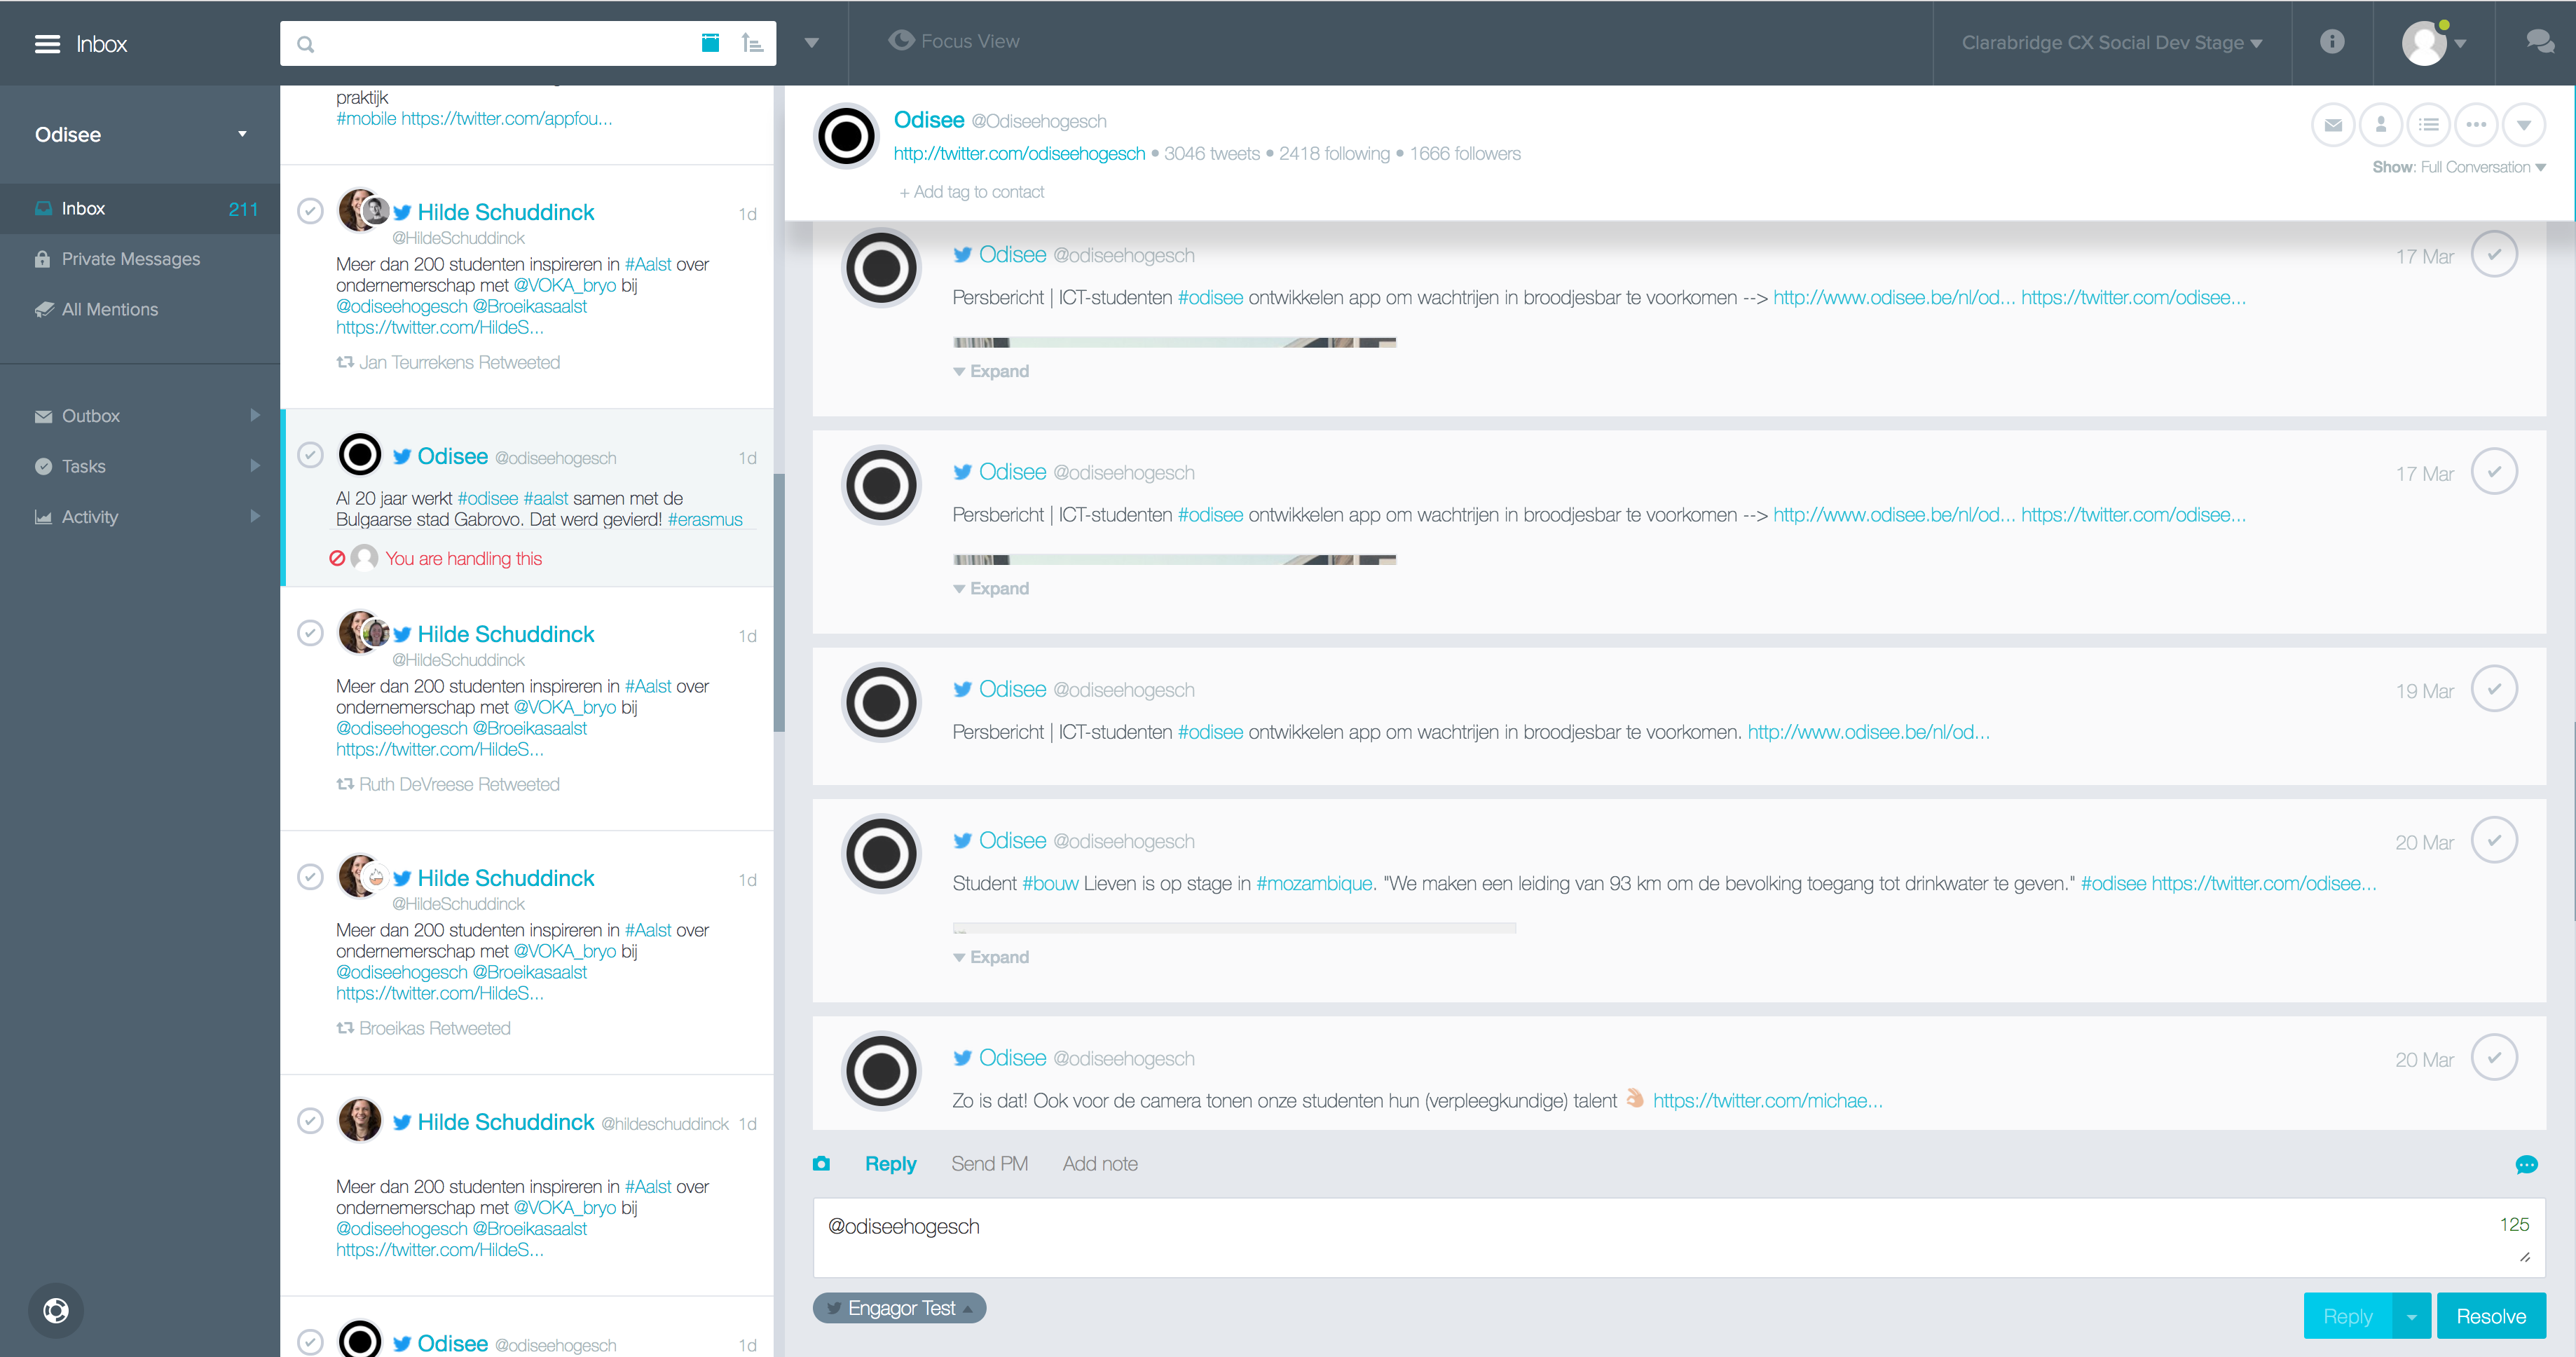
\includegraphics[width=1\textwidth]{Figuren/Inbox.png}
	\caption{Inbox CX Social \cite{EngagorScreenshots}} %\cite{Pouladzadeh}
	\label{fig:Inbox}
\end{figure} 

Via de `Insights' kunnen bedrijven ook de statistieken van hun pagina's bijhouden. Zo zijn de totale mentions van een \textit{topic} te zien alsook de \textit{mentions} per pagina. Dit alles wordt zeer intu\"{i}tief  weergegeven in de vorm van cirkeldiagrammen en tijdlijnen. Hier wordt ook het sentiment berekend. Dit geeft een aanduiding van het percentage van de mentions die een positieve, negatieve of neutrale connotatie hebben. Ook trends (veelgebruikte woorden, hashtags  etc.) en foto's die binnen een topic voorkomen zijn hier te vinden (zie Figuur~\ref{fig:Insights}).  

\begin{figure}[H]
	\centering
	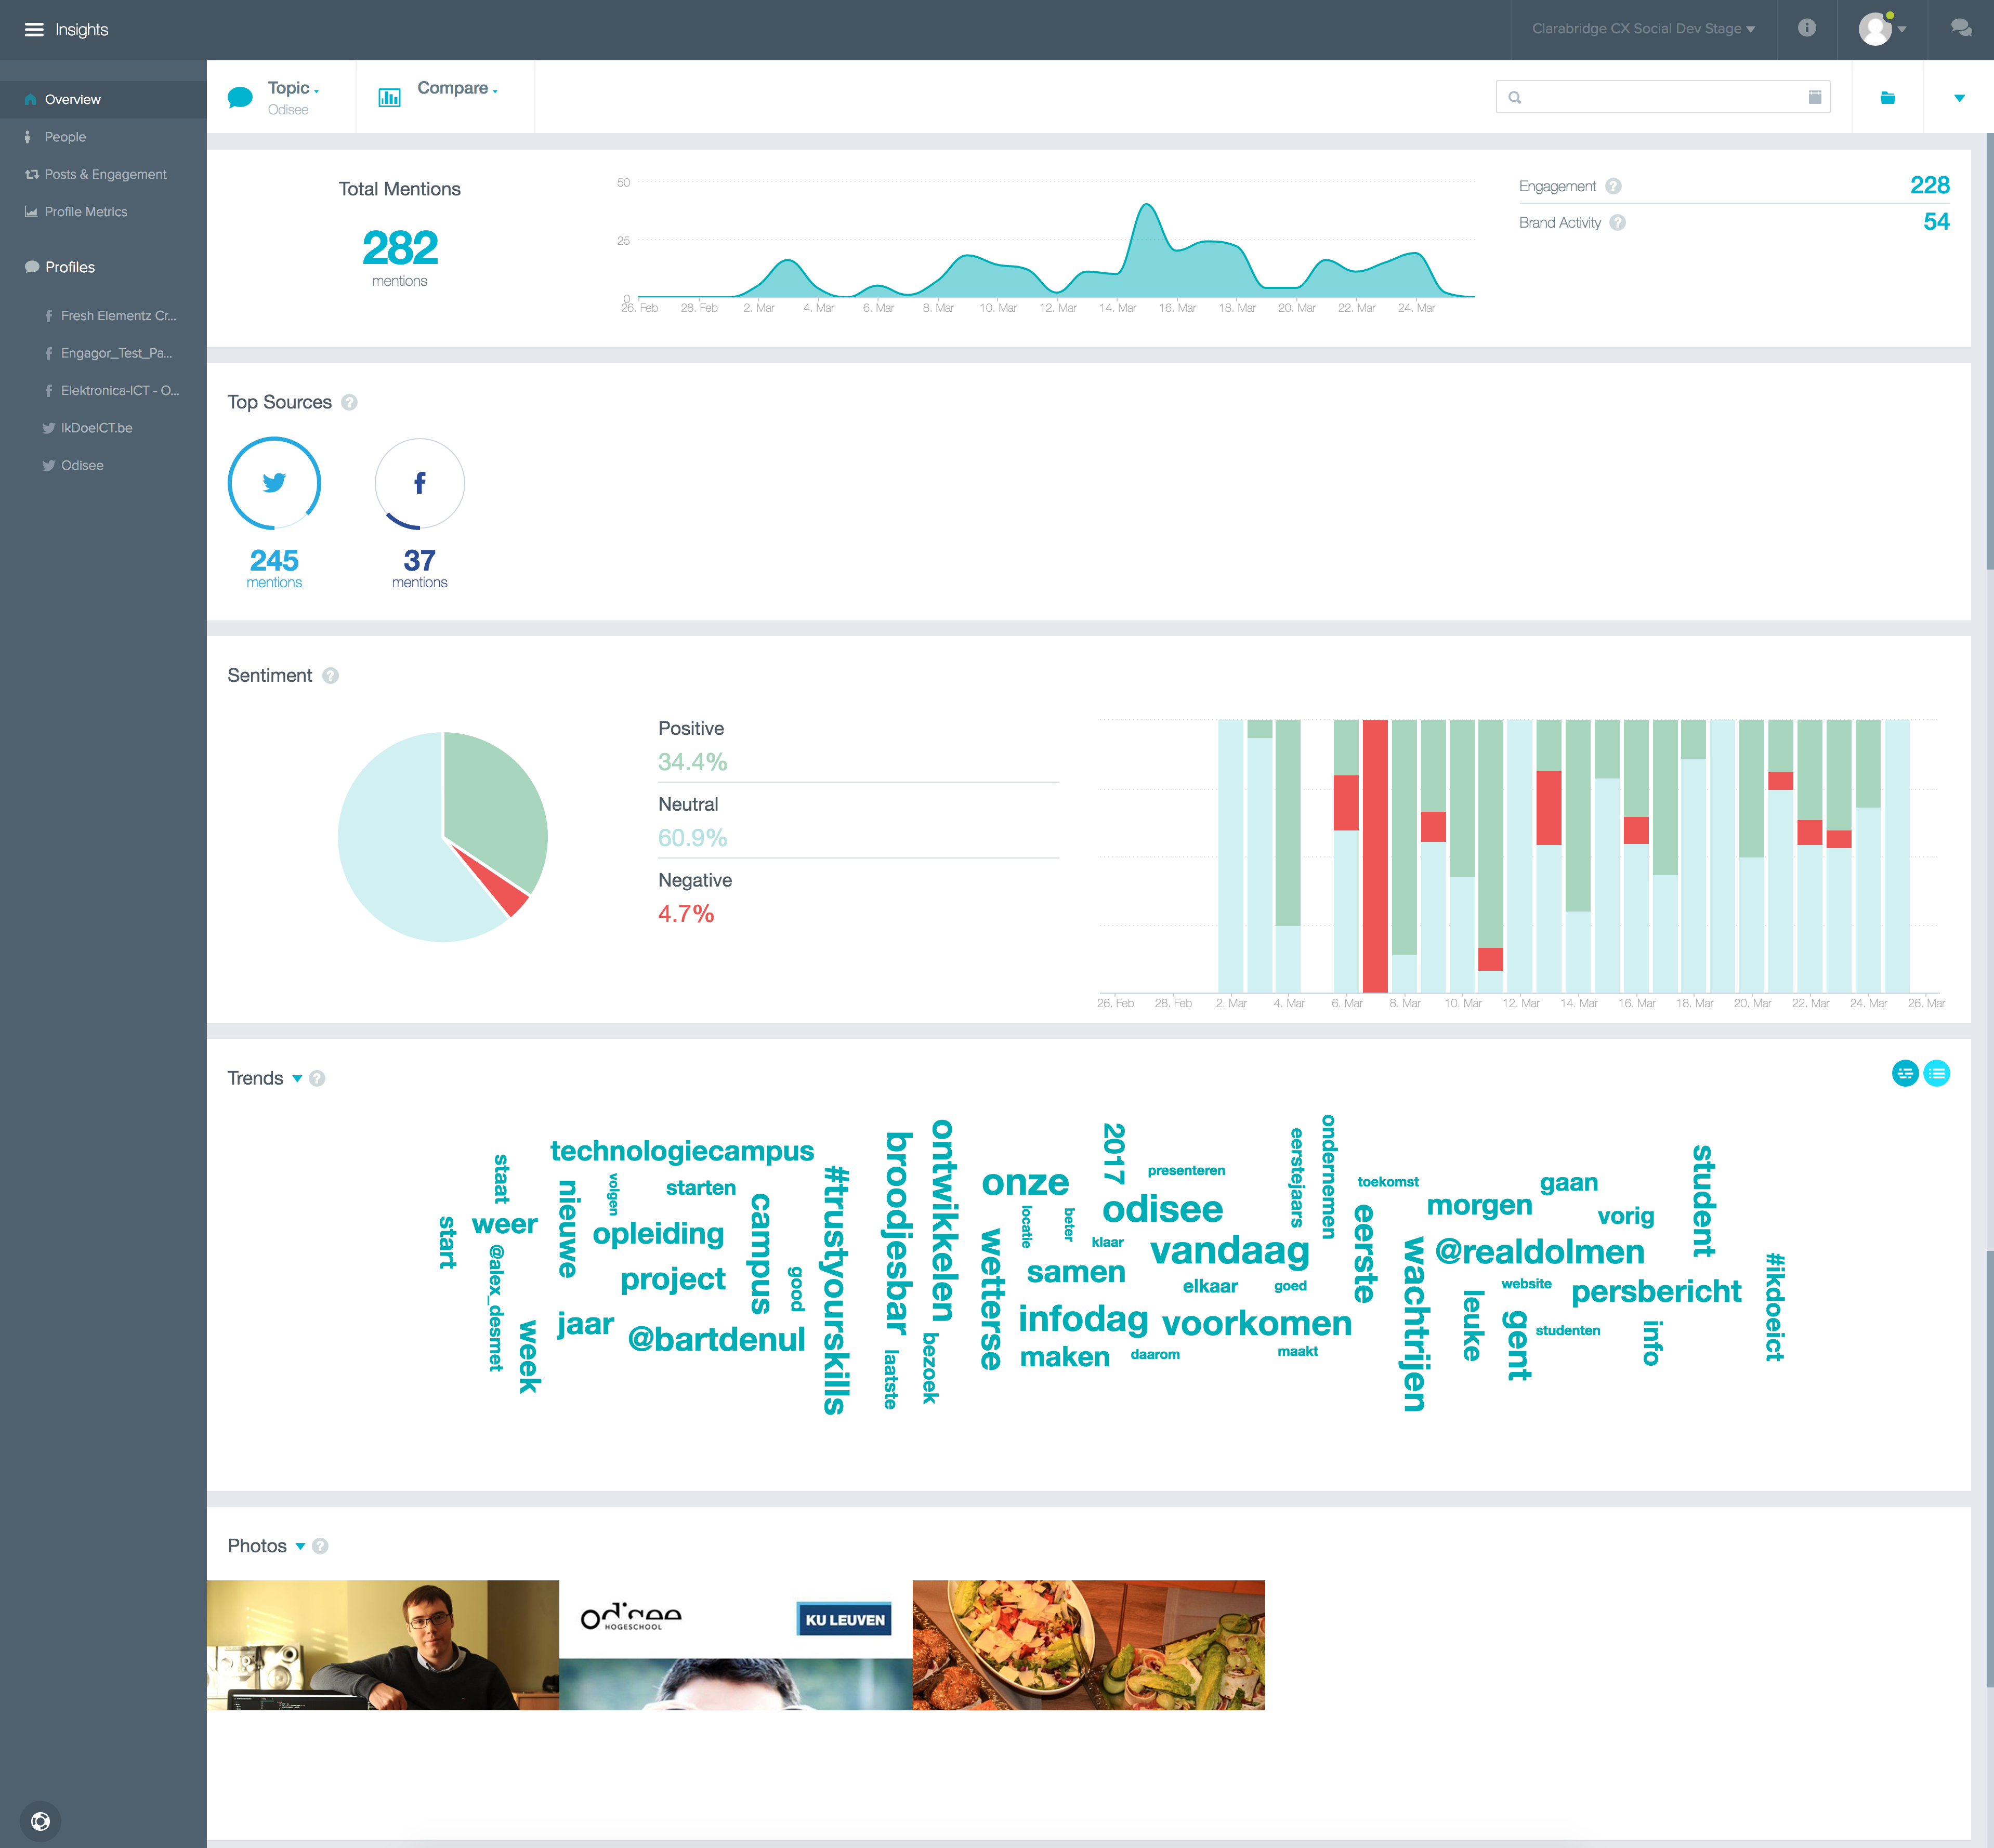
\includegraphics[width=1\textwidth]{Figuren/Insights.png}
	\caption{Insights CX Social \cite{EngagorScreenshots}} %\cite{Pouladzadeh}
	\label{fig:Insights}
\end{figure} 

Nog meer statistieken zijn terug te vinden op de `Performance' pagina. Hier is bijvoorbeeld te zien hoe lang het duurde voor actie werd ondernomen, hoeveel unieke gebruikers geholpen werden of hoeveel antwoorden gemiddeld gegeven werden op een mention (zie Figuur~\ref{fig:Performance}).

\begin{figure}[H]
	\centering
	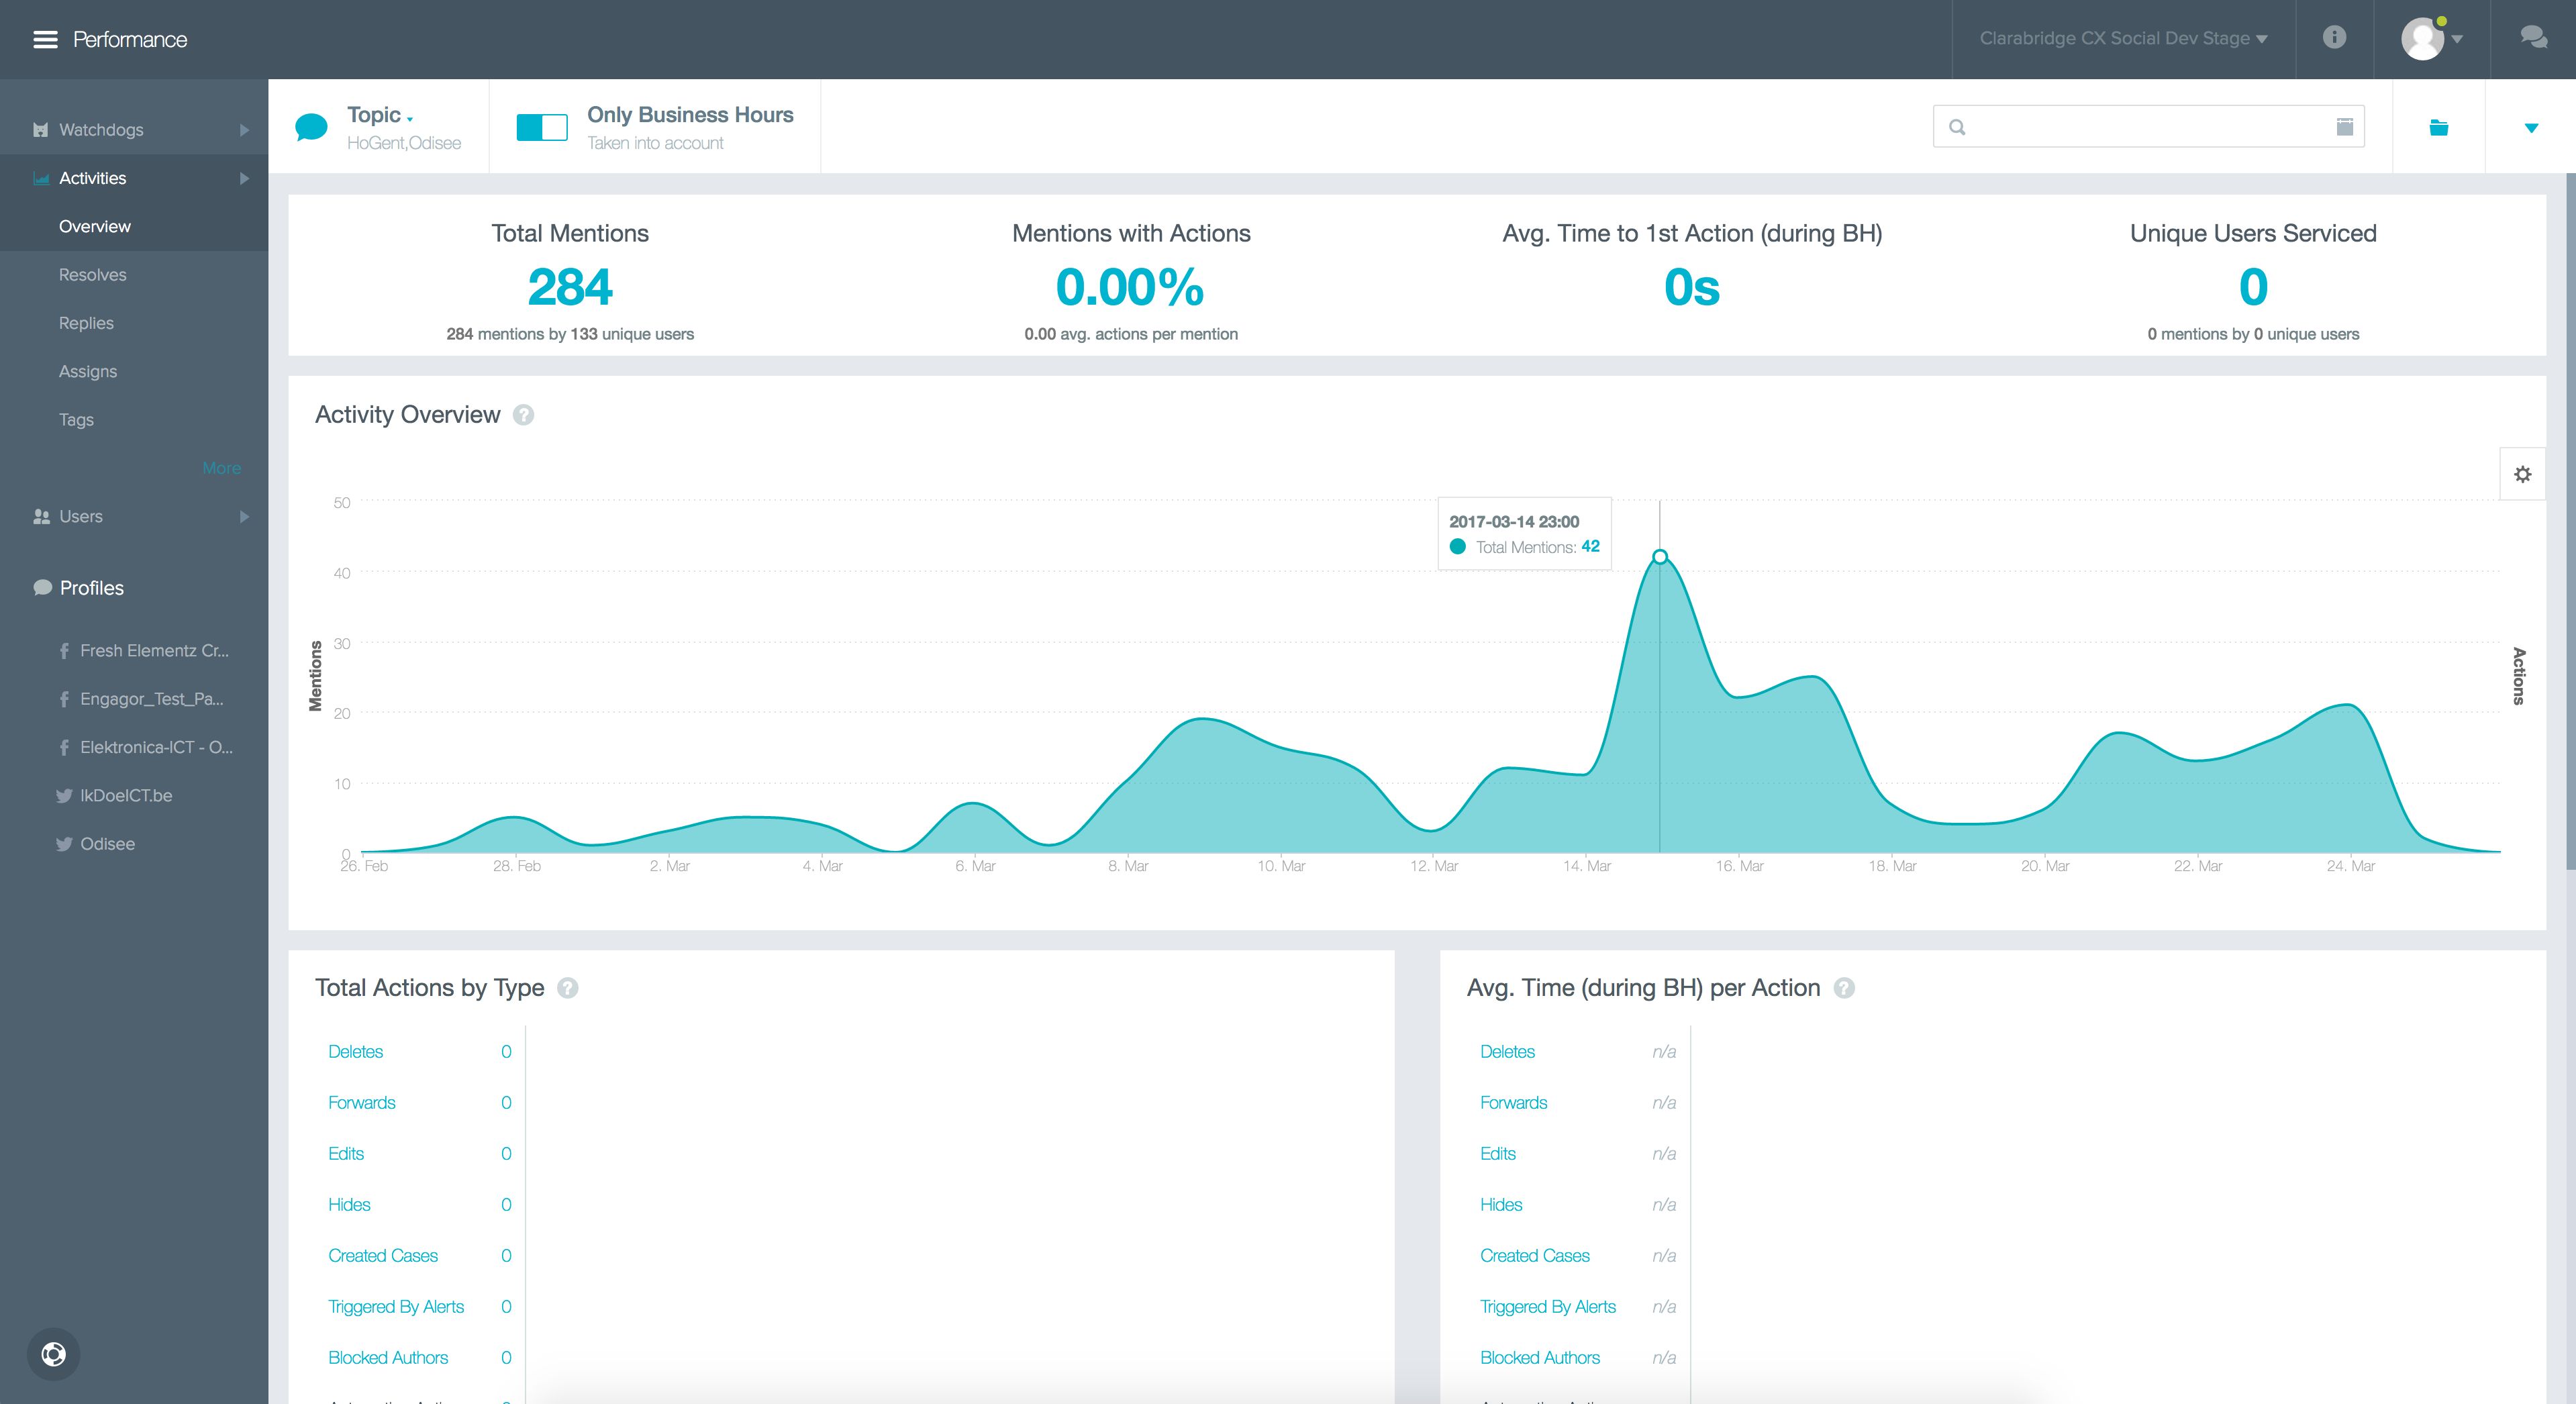
\includegraphics[width=1\textwidth]{Figuren/Performance.png}
	\caption{Performance CX Social \cite{EngagorScreenshots}} %\cite{Pouladzadeh}
	\label{fig:Performance}
\end{figure} 


Niet enkel berichten kunnen beheerd worden via de webapplicatie maar er kan ook gepost worden op profielen zelf. Dit kan per topic en per profiel gebeuren. Posts kunnen ook gepland worden om ze op een later tijdstip op het profiel weer te geven  of opgeslagen worden als \textit{canned response}. Dit zijn standaard antwoorden die gebruikt kunnen worden tijdens het communiceren met klanten \cite{EngagorApp}. Zo kunnen klanten sneller geholpen worden met hun problemen.
 
\chapter{Probleemstelling}
\vspace{-3cm}
\section{Probleemstelling vanuit de stage} \label{BeschrijvingStageOpdracht}

Als stageopdracht dient een nieuwe feature toegevoegd te worden aan de CSXSocial webapplicatie: een \textit{profile manager}. Deze \textit{profile manager} moet gebruikers in staat stellen de profielfoto en/of omslagfoto van een profiel in te stellen. Dit gebeurt aan de hand van thema's. Een thema kan aangemaakt worden voor een specifieke service, bijvoorbeeld Facebook of Twitter. Voor Facebook kan een thema een omslagfoto en een profielfoto bevatten terwijl een thema voor Twitter naast de foto's ook de link kleur, naam en bio kan bevatten (zie Figuur~\ref{fig:EditTheme}). Het moet ook mogelijk zijn voor de klanten om deze afbeeldingen te passen. Zo kunnen ze tekst toevoegen aan de afbeelding of hun eigen \textit{Key Performance Indicator} (KPI)\footnote{Een \textit{Key Performance Indicator} is een meetbare waarde waarmee de prestaties van bedrijven of ondernemingen uitgedrukt worden. Binnen CXSocial zijn dit bijvoorbeeld de geholpen klanten per dag of hoe lang het gemiddeld duurt voor klanten geholpen worden} er op plaatsen. Aangezien de omslagfoto's van Facebook en Twitter niet dezelfde dimensies bezitten en de foto ook niet op volledige grootte aan de gebruikers kan getoond worden, zullen de afbeeldingen ook herschaald moeten worden naar de correcte dimensies.

\begin{figure}[H]
	\centering
	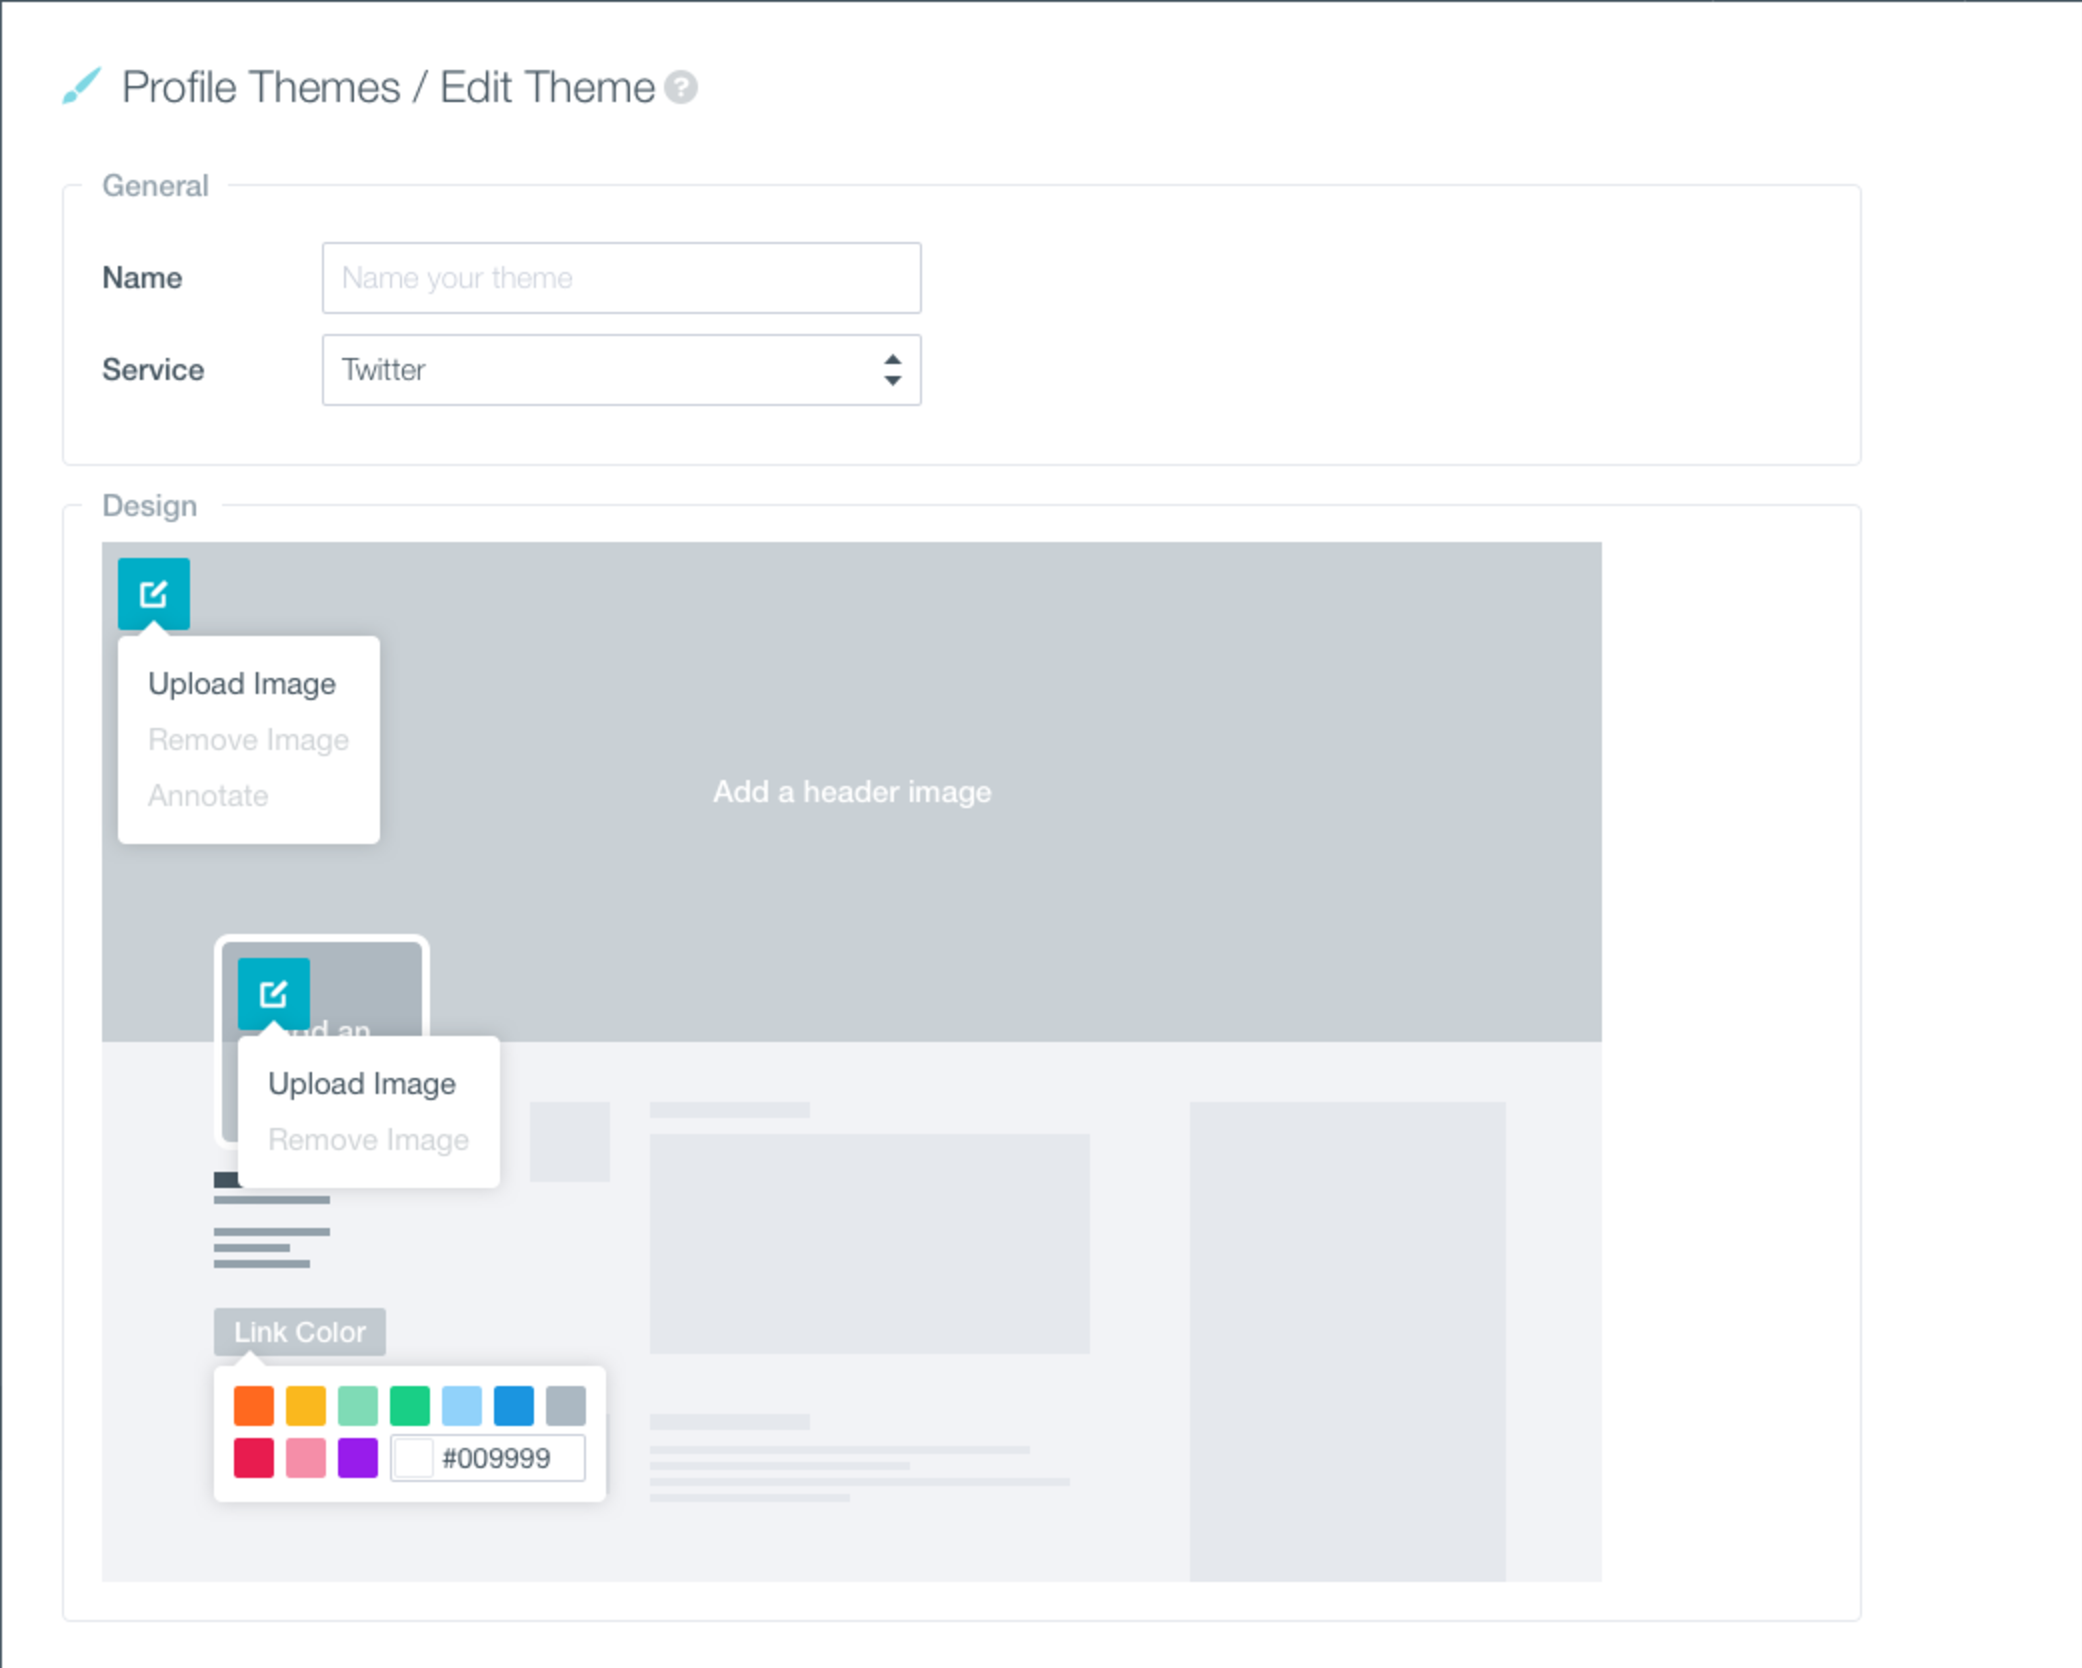
\includegraphics[width=0.7\textwidth]{Figuren/EditThemeMockup.png}
	\caption{Mockup van de editeerpagina \cite{EditThemeMockup}} %\cite{Pouladzadeh}
	\label{fig:EditTheme}
\end{figure} 

Verschillende thema's moeten aan een planning toegevoegd kunnen worden. Een klant kan dan instellen dat een bepaald thema ofwel binnen de \textit{business hours} gebruikt wordt ofwel tijdens een bepaalde periode ofwel tijdens beide. Een speciaal thema voor bijvoorbeeld Kerstmis kan dan ingesteld worden om tijdens de kerstperiode ingesteld te zijn op het profiel. Wanneer meerdere thema's op een profiel zijn ingesteld, moet dus berekend worden welk van deze thema's op een gegeven moment toegepast moet worden. 

\newpage
De webapplicatie bezit ook \textit{Crisis Plans}. Dit zijn instellingen die bij een probleem binnen het bedrijf actief gesteld kunnen worden. Eens actief wordt een waarschuwing getoond, rechten van gebruikers verandert of een to-do lijstje opgesteld met stappen die ondernomen moeten worden om het probleem op te lossen. Via een \textit{Crisis Plan} moet ook een thema ingesteld kunnen worden. Een gebruiksscenario hiervoor zou bijvoorbeeld kunnen zijn: het instellen van een specifieke omslagfoto en avatar wanneer een bedrijf kampt met een technische storing. 

\section{Probleemstelling bachelorproef}

Deel van de stageopdracht is het verwerken van afbeeldingen om als omslagfoto of avatar te gebruiken. Hierbij is het de bedoeling dat klanten afbeeldingen kunnen uploaden die dan als omslagfoto en/of avatar zullen dienen. Een thema, bestaande uit deze afbeeldingen en in sommige gevallen nog enkele andere variabelen zoals link kleur voor een Twitter profiel, kunnen ingesteld worden om op bepaalde tijdstippen actief te zijn. Klanten moeten in staat zijn tekst en KPI's op deze afbeeldingen te plaatsen vanuit de webapplicatie. De afbeeldingen moeten samengesteld kunnen worden door de gebruiker maar moeten nadien ook opnieuw gegenereerd kunnen worden op de server met aangepaste KPI's. 

Om afbeeldingen te annoteren is redelijk wat functionaliteit nodig. Ingegeven tekst moet eender waar op een afbeelding geplaatst kunnen worden maar moet ook gestyled kunnen worden. Lettertype, kleur, lettergrootte, gewicht en uitlijning moeten allemaal ingesteld kunnen worden door gebruikers. Dit moet zowel clientside als serverside mogelijk zijn aangezien de KPI's telkens zullen veranderen waardoor nieuwe afbeeldingen gegeneerd moeten worden. 

Naast het genereren van de afbeeldingen moeten deze ook ge\"{u}pload worden naar Facebook of Twitter op de ingestelde tijdstippen. Er moet dus geregeld berekend worden welke afbeelding met welke KPI's op een bepaald tijdstip ingesteld moet worden als omslagfoto. De gebruiker verwacht natuurlijk dat telkens de correcte foto op het profiel ingesteld is waardoor de betrouwbaarheid ook een zeer belangrijk punt is. In functie van de bachelorproef worden bibliotheken en technologie\"{e}n bestudeert en vergeleken.  


%MSS OPNIEUW SCHRIJVEN? VORIGE ZINNEN?
%In functie van de bachelorproef zullen blablabala
%Bibliotheken en technologie\"{e}n zullen onderzocht worden om dit alles te kunnen verwezenlijken.


%NOG E BTJ BIJSCHRIJVEN!!

\iffalse
\chapter{Stageopdracht}
\vspace{-3cm}
Als stageopdracht dient een nieuwe feature toegevoegd te worden aan de webapplicatie: een \textit{profile manager}. Deze \textit{profile manager} moet gebruikers in staat stellen de profielfoto en/of omslagfoto van een profiel te veranderen. Dit gebeurt aan de hand van thema's. Een thema kan aangemaakt worden voor een specifieke service, bijvoorbeeld Facebook of Twitter. Voor Facebook kan een thema een omslagfoto en een profielfoto bevatten terwijl een thema voor Twitter naast de foto's ook de link kleur, naam en bio kan bevatten (zie Figuur~\ref{fig:EditTheme}). Het moet ook mogelijk zijn voor de klanten om deze afbeeldingen te passen. Zo kunnen ze tekst toevoegen aan de afbeelding of hun eigen \textit{Key Performance Indicators} (KPI) er op plaatsen. Aangezien de omslagfoto's van Facebook en Twitter niet dezelfde dimensies bezitten en de foto ook niet op volledige grootte aan de gebruikers kan getoond worden, zullen ook de afbeeldingen herschaald moeten worden.

Verschillende thema's moeten ook aan een planning toegevoegd kunnen worden. Een klant kan instellen dat een bepaald thema ofwel binnen de \textit{business hours} gebruikt wordt ofwel tijdens een bepaalde periode ofwel tijdens beide. Een speciaal thema voor bijvoorbeeld Kerstmis kan dan ingesteld worden om tijdens de kerstperiode ingesteld te zijn op het profiel. 

De webapplicatie bezit ook \textit{Crisis Plans}. Dit zijn instellingen die bij een probleem actief gesteld kunnen worden. Eens actief wordt een waarschuwing getoond, rechten van gebruikers verandert of een to-do lijstje opgesteld met stappen om het probleem op te lossen. Via een \textit{Crisis Plan} moet ook een thema ingesteld kunnen worden. Een gebruiksscenario hiervoor zou bijvoorbeeld kunnen zijn: het instellen van een specifieke omslagfoto en avatar wanneer een bedrijf kampt met een technische storing. 

\begin{figure}[H]
	\centering
	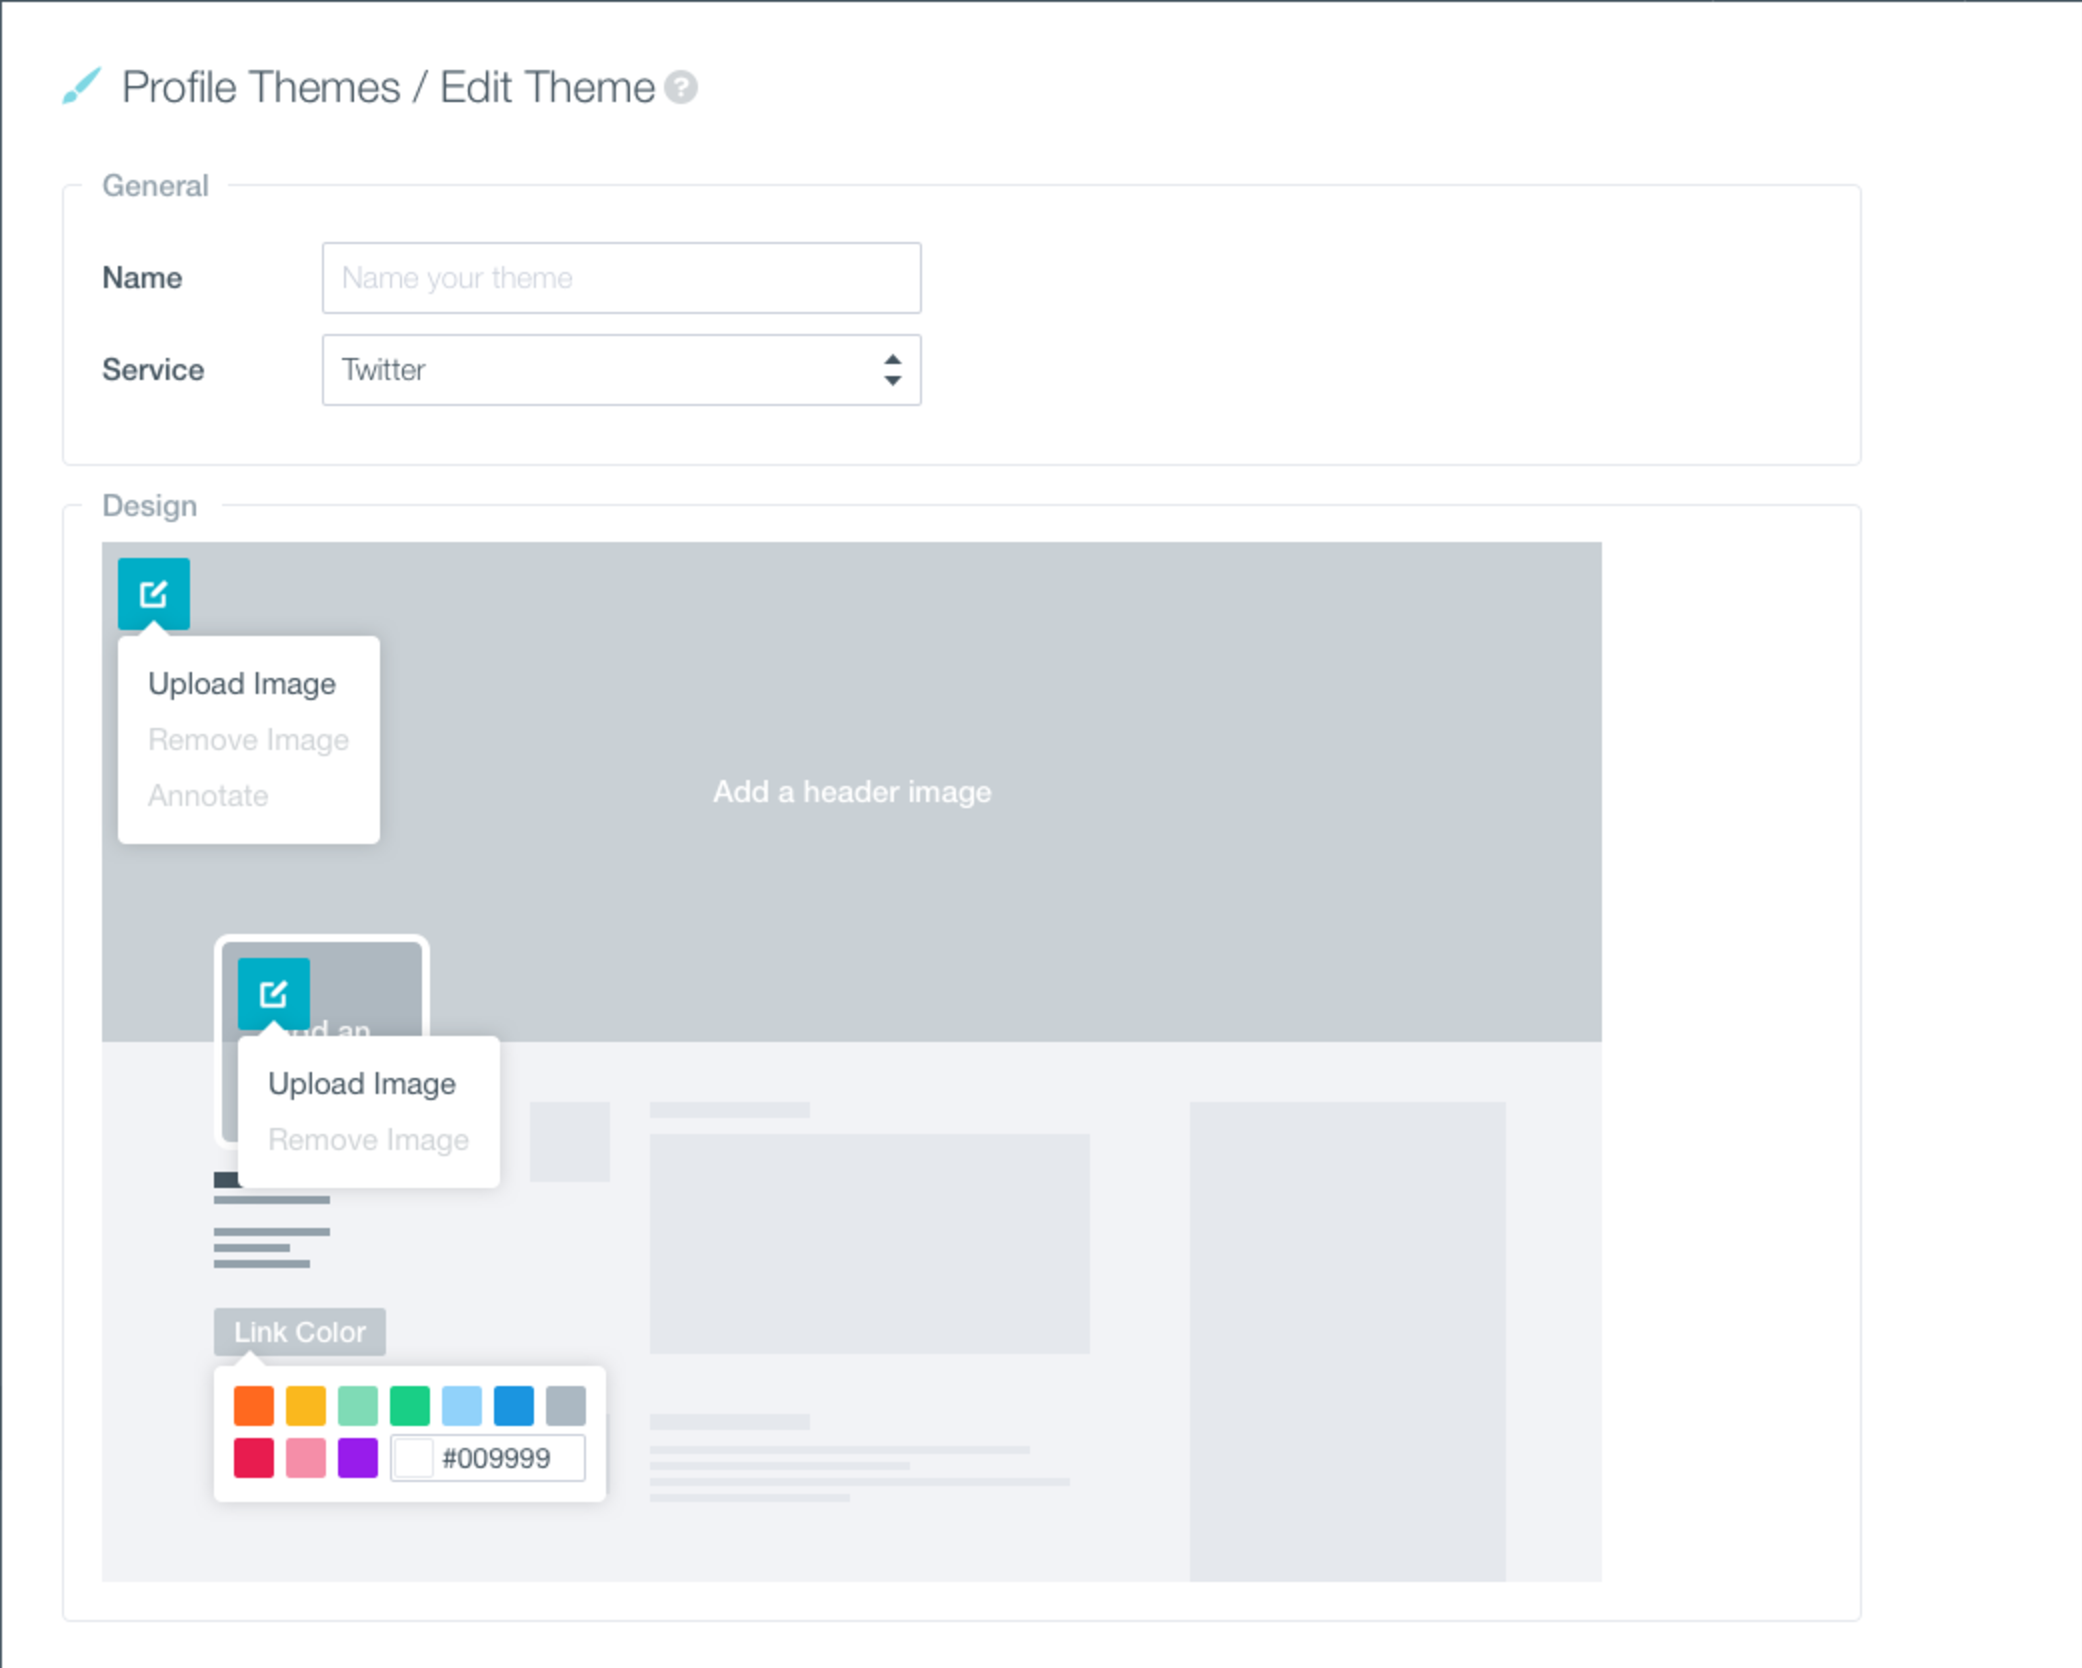
\includegraphics[width=0.6\textwidth]{Figuren/EditThemeMockup.png}
	\caption{Mockup van de editeerpagina \cite{EditThemeMockup}} %\cite{Pouladzadeh}
	\label{fig:EditTheme}
\end{figure} 

\chapter{Omschrijving bachelorproef}
\vspace{-3cm}
Deel van de stageopdracht is het verwerken van afbeeldingen om als omslagfoto of avatar te gebruiken. Hierbij is het de bedoeling dat klanten afbeeldingen kunnen uploaden die dan als omslagfoto en/of avatar zullen dienen.  Een thema, bestaande uit deze afbeeldingen en in sommige gevallen nog enkele andere variabelen zoals link kleur, info of naam van het profiel, kunnen ingesteld worden om op bepaalde tijdstippen actief te zijn. Klanten moeten in staat zijn tekst en KPI's op deze afbeeldingen te plaatsen vanuit de webapplicatie. De afbeeldingen moeten samengesteld kunnen worden door de gebruiker maar moeten nadien ook opnieuw gerenderd kunnen worden met aangepaste KPI's. Dit moet dus op de server gebeuren. 

Om afbeeldingen te annoteren is redelijk wat functionaliteit nodig. Ingegeven tekst moet eender waar op een afbeelding geplaatst kunnen worden maar moet ook gestyled kunnen worden. Gebruikers moeten alle basiseigenschappen van een stuk tekst kunnen aanpassen. Lettertype, kleur, lettergrootte, gewicht en uitlijning moeten allemaal ingesteld kunnen worden door gebruikers. Dit moet zowel clientside als serverside mogelijk zijn. Bibliotheken en technologie\"{e}n zullen onderzocht worden om dit te kunnen verwezenlijken.
\fi  


{\renewcommand{\arraystretch}{1.4}
\begin{landscape}
\chapter{Actieplan}
	\vspace{-3cm}
	
	\begin{table}[htbp]
		\centering
		\begin{tabular}{|l|p{0.5\linewidth}|l|l|l|}
			\hline
			\multicolumn{1}{|c|}{\textit{\textbf{Milestones}}}&
			\multicolumn{1}{|c|}{\textit{\textbf{Taak}}}&
			\multicolumn{1}{|c|}{\textit{\textbf{Start datum}}} & \multicolumn{1}{c|}{\textit{\textbf{Eind datum}}} &
			\multicolumn{1}{c|}{\textit{\textbf{Duur}}} \tabularnewline \hline
			Milestone 1 & Defining Architecture/Data Model & 6/02/2017 & 10/02/2017 & 4\tabularnewline \hline
			Milestone 2 & Test scripts for uploading avatars/cover photos for Faceboo/Twitter & 13/02/2017 & 17/02/2017 & 4\tabularnewline \hline
			Milestone 3 & Theme creation (Name, Type, Images, Link color) & 20/02/2017 & 24/02/2017 & 4\tabularnewline \hline
			Milestone 4 & Selecting multiple themes for profiles & 27/02/2017 & 03/03/2017 & 4\tabularnewline \hline
			Milestone 5 & Applying thems (cron jobs/scheduled) & 06/03/17 & 10/03/17 & 4\tabularnewline \hline
			Milestone 6 & Update profile name/link/bio (Twitter) & 13/03/17 & 17/03/17 & 4\tabularnewline \hline
			Milestone 7 & Annotations & 20/03/17 & 7/04/17 & 12\tabularnewline \hline
			Milestone 8 & Annotations with KPI & 20/03/17 & 7/04/17 & 12\tabularnewline \hline
			Milestone 9 & Define welcome messages for profile (Optional) & 10/04/17 & 21/04/17 & 8\tabularnewline \hline
			Milestone 10 & Define persistent menu for Facebook (Optional) & / & / & /\tabularnewline \hline
			Milestone 11 & Integration in Crisis Plans & 24/04/17 & 28/04/17 & 4\tabularnewline \hline
			Milestone 12 & Theme preview (Optional) & / & / & /\tabularnewline \hline
			Milestone 13 & Asset Gallery in Theme Builder (Optional) & / & / & /\tabularnewline \hline
			Milestone 14 & Depolyment & 1/05/17 & 5/05/17 & 4\tabularnewline \hline
			Milestone 15 & Testing & 8/05/17 & 12/05/17 & 4\tabularnewline \hline
			 
		\end{tabular}
		\caption{Milestones Profile Manager}
		\label{tabelActieplan}   
	\end{table}
	
	
	
	\newpage
	
	\begin{figure}[H]
		\centering
		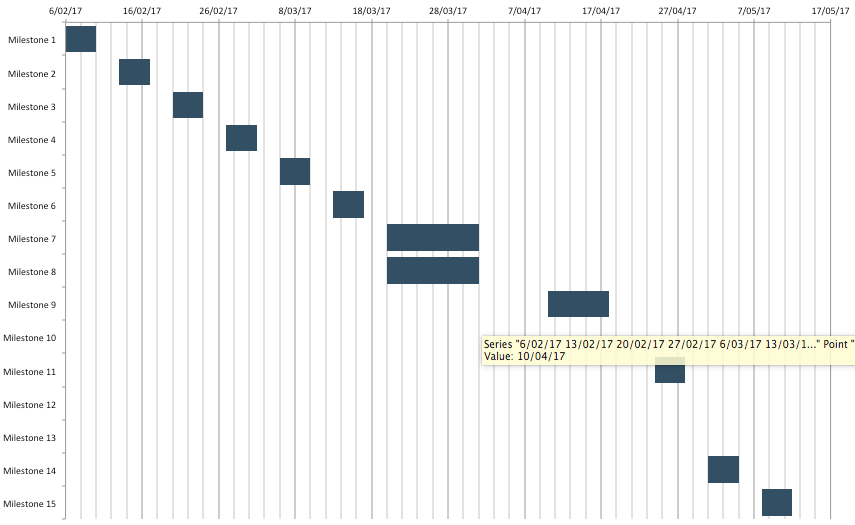
\includegraphics[width=1.5\textwidth]{Figuren/GanttChartDark.png}
		\caption{Gantt chart - Profile Manager} %\cite{Pouladzadeh}
		%\label{fig:Actieplan}
	\end{figure}
\end{landscape}

\chapter{Voorstudie}
\vspace{-3cm}
\section{Vereisten} \label{vereisten}
Alle bibliotheken en technologie\"{e}n die besproken zullen worden, moeten aan enkele voorwaarden voldoen. Zo moeten afbeeldingen en tekst: verplaatst, geschaald, geroteerd en over elkaar geplaatst kunnen worden (wat dus inhoudt dat de gebruikte bibliotheek/technologie 'lagen' moet ondersteunen). Idealiter kan tekst, eens op het canvas geplaatst, nog aangepast worden. Dit vooral om interactie met tekst voor de gebruikers eenvoudiger te maken. Nadien moeten de afbeeldingen ge\"{e}xporteerd en hun eigenschappen (tekst, KPI's, kleur, lettertype etc.) bewaard kunnen worden. Aangezien KPI's aanwezig zijn op de afbeelding, moeten deze later ook aangepast kunnen worden. De afbeeldingen zullen dus om de zoveel tijd opnieuw gegenereerd worden met nieuwe, aangepaste KPI`s. 

Veel sociale media verwachten dat omslag-en profielfoto's bepaalde dimensies bezitten. De vereiste dimensies van omslagfoto's kunnen redelijk groot uitvallen om problemen met schaling te voorkomen. Twitter verwacht bijvoorbeeld een afbeelding van 1500 op 500 pixels. Dit is natuurlijk niet gebruiksvriendelijk weer te geven in een browservenster. Daarom moet herschalen van het volledige canvas met elk van zijn objecten mogelijk zijn. Hierbij is het belangrijk dat alle verhoudingen behouden blijven om uiteindelijk dezelfde afbeelding te bekomen zoals die door de gebruiker gemaakt werd. Naast de frontend manipulatie van afbeeldingen zal dus ook manipulatie in de backend onderzocht moeten worden.  

\section{Frontend afbeelding manipulatie}
Redelijk wat bibliotheken om afbeeldingen te manipuleren zijn reeds te vinden. De meeste hiervan zijn gericht op het gebruiken van filters op afbeeldingen of het maken van animaties in een canvas. Hoewel deze bibliotheken veel te bieden hebben, zijn ze minder geschikt voor deze toepassing. Het is hier namelijk de bedoeling om elementen op een canvas te positioneren, zowel tekst als de afbeeldingen zelf. Het volledige canvas en alle inhoud moet op gepaste wijze opgeslagen kunnen worden zodat het canvas op een later tijdstip opnieuw opgebouwd kan worden. 

\subsection{Fabric.js}
Een bibliotheek die onmiddellijk veelbelovend lijkt te zijn is Fabric.js. Het is een JavaScript bibliotheek die HTML5 canvas manipulatie gemakkelijker maakt. Het maakt het mogelijk om object-geori\"{e}nteerd te werken binnen een canvas in plaats van simpelweg vormen te `tekenen' op het canvas. Dit maakt het veel gemakkelijker om complexe interacties met het canvas uit te voeren. Selecteren, verplaatsen, herschalen, roteren en dergelijke transformaties kunnen ondernomen worden zonder veel problemen. 

\textbf{Functionaliteit} \break 
In plaats van te functioneren op de context van het canvas zal Fabric gebruik maken van objecten die aan het canvas toegevoegd worden \cite{FabricJSDocs}. Fabric bezit zeven verschillende standaard vormen: cirkels, ellips, lijn, polygon, polylijn, rechthoek en driehoek.

Alle objecten erven over van het \textit{root object}. Dit stelt een tweedimensionale vorm voor in het tweedimensionaal canvas en bezit een positie in het canvas (x-en y-co\"{o}rdinaat), een hoogte en een breedte. Aangezien elk objct dus overerft van deze klasse, ontstaat een soort van hi\"{e}rarchie en kunnen methodes geschreven worden die bruikbaar zijn voor elke instantie van een object \cite{FabricJSIntro}. 

Interessanter voor deze implementatie zijn de tekst en afbeelding objecten. Naast het gewone \texttt{fabric.Text} object, wat enkel statische tekst voorstelt, is ook de \texttt{fabric.IText} beschikbaar. Met dit object kan interactieve tekst aan het canvas toegevoegd worden. Deze tekst kan dus in het canvas zelf aangepast worden. Het Text object bezit properties om: grootte, stijl (vet/schuin/normaal), gewicht en lettertype aan te passen. Het standaard HTML canvas bezit slechts twee methodes om tekst te renderen: \texttt{strokeText(text, x, y [, maxWidth])} en \texttt{fillText(text, x, y [, maxWidth])} \cite{MozillaCanvas-DrawingText}. 
%De eerste methode zal ingevulde tekst op het canvas tekenen op de meegegeven x-en y-positie. De tweede zal enkel de omtrek van de meegegeven tekst op het canvas tekenen. Naast deze methodes zijn ook heel wat eigenschappen beschikbaar zoals font (e.g. 20px comic-sans), textAlign (e.g. center), textBaseline (e.g. alphabetic) en direction (e.g. ltr). Functionaliteit hiervan is eerder beperkt.
Naast deze methodes zijn ook heel wat eigenschappen beschikbaar waaronder lettertype, uitlijning, textBaseline (e.g. alphabetic) en richting (e.g. ltr). Functionaliteit hiervan is eerder beperkt en zeker niet uitgebreid genoeg om aan de gestelde eisen (zie sectie \ref{vereisten}) te kunnen voldoen. 

Het tekst object dat Fabric voorziet voegt heel wat nieuwe functionaliteit toe zoals: multiline ondersteuning, tekst decoratie, uitlijning, lijnhoogte en meer.

\iffalse
\begin{itemize}
	\item Multiline ondersteuning
	\item Tekst achtergrond
	\item Tekst decoratie
	\item Uitlijning
	\item Lijnhoogte
\end{itemize}
\fi

Vooral ondersteuning van multiline tekst en uitlijning hiervan zijn zeer handige \textit{features}. Alle objecten op het canvas kunnen \textit{by default} geselecteerd en verplaatst worden. Natuurlijk is dit met het standaard canvas element ook mogelijk, maar code hiervoor zou steeds complexer worden naarmate meer functionaliteit toegevoegd wordt.

%CHECK OF EVENT IS ITALIC OF NIET THROUGHOUT BP!
Het \textit{draggable} of verplaatsbaar maken van tekst in een standaard HTML canvas, vereist heel wat code. Alle tekst, die op het canvas geplaatst wordt, moet bijgehouden worden in een lijst of array. Wanneer een \textit{mouse-down} event plaatsvindt, moet berekend worden of de klik daadwerkelijk op een item in het canvas gebeurde. Is dit het geval dan moet de index van het geselecteerde item opgeslagen worden. Bij het triggeren van een \textit{mouse-move} event moeten de co\"{o}rdinaten van dit item aangepast worden naar deze van de cursor, waarna ieder item terug op het canvas getekend moet worden. 

\begin{lstlisting}[language=javascript]
	document.getElementById('addTextButton').click(function() {
	 var text = document.getElementById('text').value;
	 items.push(text);
	});
	
	document.getElementById('canvas').onmousedown = function() (
	 // Kijk wanneer positie van de cursor overeen komt met een tekst object
	)
\end{lstlisting}

Ook afbeeldingen zijn gemakkelijk te manipuleren in een Fabric canvas. Afbeeldingen kunnen geladen worden vanuit een Scalable Vector Graphics (SVG) element, een object of een URL. Met het standaard canvas element kunnen enkel afbeeldingen via URL ingeladen worden. Hoewel dit bij deze toepassing op zich niet onmiddellijk een bottleneck vormt aangezien de afbeelding ingeladen zal worden vanuit een `file server', kan het toch handig zijn om de extra functionaliteit ter beschikking te hebben. In de toekomst kan het bijvoorbeeld nodig zijn om een SVG afbeelding te cre\"{e}ren en in te laden in het canvas. Dan moet, bij het gebruik van Fabric, geen ander script/bibliotheek ge\"{i}nstalleerd worden om deze functionaliteit te verkrijgen. Het fabric.Image object bezit heel wat methodes die het gebruik van afbeeldingen net dat beetje eenvoudiger maken. De \texttt{scaleToWidth()} functie kan gebruikt worden om de afbeelding de volledige breedte van het canvas te laten innemen. Manipulatie van een object kan ook afgesloten worden. 
%Zo zijn er de \texttt{lockMovementX()}, \texttt{lockMovementY()}, \texttt{lockScalingX}, \texttt{lockScalingY} en \texttt{lockRotation} methodes die bij het renderen van achtergrondafbeeldingen zeer nuttig kunnen zijn. Het is namelijk handig om de acties van de gebruiker wat in te kunnen perken. Door enkele bewegingen te locken wordt het dus onmogelijk om bijvoorbeeld de afbeelding uit het zichtbare gedeelte van het canvas te slepen. 
Naast de mogelijkheid tot inladen van afbeeldingen, kunnen hierop ook filters toegepast worden. Hoewel dit momenteel geen vereiste is voor het project, zou dit in de toekomst toegevoegd kunnen worden. Het Image object beschikt over de meest courante filters zoals helderheid, contrast, grijstinten, sepia, ruis en inverteren.  

Een belangrijke vereiste is de ondersteuning van lagen aangezien tekst bovenop de afbeelding geplaatst moet kunnen worden. Hiervoor bezit Fabric verschillende methodes. Objecten kunnen een positie hoger of lager in de stack van objecten, die op dat moment op het canvas aanwezig zijn, geplaatst worden met behulp van de \lstinline|sendBackwards(object)| of \lstinline|bringForward(object)| methodes. Deze methodes bezitten een optionele \textit{intersecting} parameter \texttt{(boolean)} die het object net voor of na het volgende snijdende object in de stack zal plaatsen (zie Figuur~\ref{fig:FabricLayers}). 

\begin{figure}[H]
	\centering
	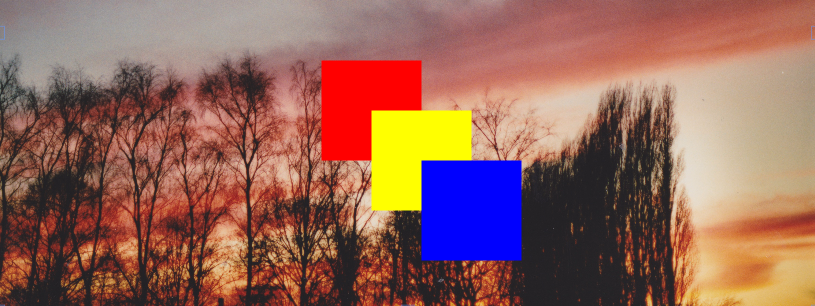
\includegraphics[width=1\textwidth]{Figuren/FabricLayers.png}
	\caption{Lagen in Fabric.js} %\cite{Pouladzadeh}
	\label{fig:FabricLayers}
\end{figure} 

Het canvas bezit ook twee methodes om objecten volledig onderaan of bovenaan de stack te plaatsen: \texttt{sendToBack(object)} en \texttt{bringToFront(object)}. Deze methodes zijn perfect om de afbeelding in te stellen als achtergrond van het canvas. Naast deze methodes bezit het canvas ook een belangrijke property, \texttt{preserveObjectStacking}. Wanneer \texttt{true} zal de positie van alle objecten op de stack bewaard blijven. Dit zorgt er voor dat objecten niet plots bovenaan de stack komen te staan als ze geselecteerd worden. Voor uitwerking van het project is de mogelijkheid tot het gebruiken van lagen onontbeerlijk. Het standaard canvas element bezit deze functionaliteit niet, althans niet zo naadloos ge\"{i}mplementeerd. 
%Het is wel mogelijk met wat tricks (zie sectie over vanilla js/jquery).

Misschien een van de grootste voordelen van Fabric is dat het zelf zorgt voor het renderen van het canvas wanneer een object gemanipuleerd wordt en dat de state van het canvas bijgehouden wordt. Kortweg betekend dit dat de \texttt{canvas.draw()} functie niet telkens moet aangeroepen worden wanneer een manipulatie plaatsvindt. Om de performantie te verhogen wordt het canvas standaard gecached. De invloed hiervan is vooral te merken bij het herschalen en verplaatsen van complexe objecten. %bv een SVG? 
Fabric houdt een tweede verborgen canvas bij waar de objecten reeds op aanwezig zijn. Wanneer een object gemanipuleerd wordt, wordt de gecachte versie getoond op het canvas. Dit zorgt voor een vloeiendere ervaring voor gebruikers \cite{FabricJSCaching}. Naast de mogelijkheid om de cache voor objecten aan of uit te schakelen, kan caching tijdens schalen van objecten uitgeschakeld worden met de \texttt{noScaleCache} eigenschap. Meer opties voor caching zijn beschikbaar maar deze zullen de performantie niet drastisch veranderen in dit project. Er zal namelijk altijd maar \'{e}\'{e}n afbeelding ingeladen worden en enkele tekst objecten. %Enkel bij het manipuleren van complese SVG-bestanden zou de invloed van caching duidelijk zichtbaar zijn. 

\textbf{Gebruiksgemak} \break
Fabric blijkt een erg veelzijdige bibliotheek te zijn die over zeer veel features beschikt die allen kunnen bijdragen tot een gebruiksvriendelijke implementatie. Gebruik van deze bibliotheek is eenvoudig (straightforward) en intu\"{i}tief. Na het aanmaken van een canvas object, kan een toegevoegd object onmiddellijk verplaatst, geschaald en geroteerd worden. Dit is een grote hulp tijdens het ontwikkelen, vergeleken met het standaard canvas element waarvoor meerdere event listeners aangemaakt moeten worden om gelijkaardige functionaliteit te verkrijgen. 

Belangrijk bij het gebruik van bibliotheken zijn de ondersteunde browsers \cite{Fabricsupportedbrowsers}. Fabric wordt ondersteund door volgende browsers: 
\begin{itemize}
	\item Firefox 2+
	\item Safari 3+ 
	\item Opera 9.64+
	\item Chrome (alle versies)
	\item IE10, IE11 en Edge
\end{itemize}

\textbf{Serialisatie}
Geannoteerde afbeeldingen moeten ook opgeslagen kunnen worden. Een Fabric canvas kan op verschillende manieren ge\"{e}xporteerd worden \cite{FabricJSIntro3Serialization}. Zo bezit Fabric twee basismethodes voor de serialisatie van een canvas: \texttt{toObject()} en \texttt{toJSON()}. De \texttt{toJSON()} functie geeft een JavaScript Object Notation (JSON) object terug die er als volgt uitziet:

\begin{lstlisting}[language=javascript]
 {"objects": [], "background": "rgba(0,0,0,0)"}
\end{lstlisting} 

De \textit{objects} eigenschap bevat alle informatie over de objecten die aanwezig zijn op het canvas zoals tekst, afbeeldingen en vormen. \textit{background} geeft de kleur van het canvas weer. 

%// Mss vergelijking maken tussen output van json vs output van png (canvas.toDataUrl(‘png’))

De \texttt{toObject()} methode geeft hetzelfde terug als \texttt{toJSON()} maar dan als een object. Het verkregen object is eigenlijk het resultaat van het aanspreken van de \texttt{toObject()} methode van elk element op het canvas. Bij het omzetten van een element naar een object, kan meegegeven worden welke eigenschappen het object moet bevatten via de optionele \texttt{propertiesToInclude} parameter. Wanneer een nieuwe klasse wordt toegevoegd, kan dus simpelweg de \texttt{toObject()} methode aangepast of uitgebreid worden. In de scope van dit project kan deze functionaliteit gebruikt worden om een extra eigenschap aan een object te geven die aangeeft of een object een KPI voorstelt of gewoon tekst.  

\begin{lstlisting}[language=javascript]
	text.toObject = (function(toObject) {   
	return function() {     
		return fabric.util.object.extend(toObject.call(this), {       
				kpiType: this.kpiType     
			});   
		}; 
	})(text.toObject);
\end{lstlisting}

Naast het omzetten van een canvas naar JSON of een object, kan een canvas ook als SVG ge\"{e}xporteerd worden met behulp van de \texttt{toSVG()} methode. Deze methode kan net zoals de \texttt{toObject()} methode uitgebreid worden. Het voordeel van het exporteren als SVG-bestand is dat het zonder aanpassing gebruikt kan worden in een browser of applicatie die SVG ondersteunt. Zowel JSON als het object moeten eerst in een canvas geladen worden om ze weer te geven. 

Natuurlijk is het ook mogelijk om een canvas als afbeelding te exporteren. Via de \texttt{toDataUrl()} methode kan het canvas zowel als JPEG als PNG opgeslagen worden. Via verschillende parameters van deze functie kunnen onder andere het formaat (PNG of JPEG), de kwaliteit, de schalingsfactor, de breedte en hoogte ingesteld worden.

\iffalse
Als parameter aan deze functie kunnen volgende opties meegegeven worden:

\begin{itemize}
	\item format (PNG of JPEG)
	\item quality (waarde tussen 0 en 1, enkel voor JPEG)
	\item multiplier (waarde waarmee de afbeelding geschaald moet worden)
	\item left (linker offset om bij te snijden/crop)
	\item top (offset bovenaan om bij te snijden)
	\item width 
	\item height
\end{itemize}
\fi

Omdat afbeeldingen ook KPI's kunnen bevatten, kunnen ze niet onmiddellijk ge\"{e}xporteerd worden als afbeelding. Ook moet rekening gehouden worden met de grootte van de bestanden wanneer deze terug naar de server verzonden worden. In een tekst bestand kan nu eenmaal veel meer informatie gestoken worden dan in een afbeelding van dezelfde grootte. 

Vanuit een JSON string of een SVG element kan een canvas opnieuw opgesteld worden \cite{SVGElement}. Voor beide representaties zijn twee methodes beschikbaar. JSON kan terug ingeladen worden met behulp van de \texttt{loadFromJSON()} of \texttt{loadFromDatalessJSON()} methodes, die beiden op het canvas zelf aangeroepen worden. \texttt{loadFromJson()} zal zoals verwacht gewoonweg een JSON string in het canvas laden. \texttt{loadFromDatalessJSON()} kan gebruikt worden bij het inladen van complexe Path objecten. Een pad zal heel wat informatie bevatten, die een JSON string al snel onleesbaar en gigantisch lang kan maken. Bij het inladen van een dataless JSON string zullen de complexe Path objecten via een SVG bestand opgehaald worden. Door het reduceren van lange paden tot een eenvoudig pad naar het SVG bestand is de representatie van het canvas veel compacter geworden. SVG elementen worden ingeladen via de \texttt{loadSVGFromURL()} methode, die als parameter een link naar de SVG inhoud verwacht. 


\subsection{Konva.js} 
Konva is een HTML5 Canvas JavaScript \textit{framework} dat voor zowel desktop als mobiele applicaties extra functionaliteit aan het canvas toevoegt. Vormen kunnen aan een canvas toegevoegd worden waarna deze verplaatst, herschaald en geroteerd kunnen worden. Konva startte als een GitHub fork van KineticJS, een andere HTML5 Canvas bibliotheek. Helaas wordt KineticJS momenteel niet meer onderhouden, alhoewel de laatste release wel nog gedownload kan worden. Stabiele releases zijn nog steeds beschikbaar alsook een lichtere versie van KineticJS, genaamd Concrete.js. Het bespreken van KineticJS op zich wordt hier achterwege gelaten aangezien het niet langer onderhouden wordt en vooral gericht is op het tekenen en animeren in een canvas.
%(en Konva hier toch op gebaseerd is) 

\textbf{Functionaliteit} \break
Het \textit{root} element in Konva is de stage, die gebruikt wordt als basis van een project. Deze stage kan meerdere lagen bevatten, die op hun beurt andere objecten of groepen van objecten bevatten. Elke laag in de stage bezit twee canvas \textit{renderers}. Een \textit{renderer} zal instaan voor het weergeven van alle objecten, dit is dus een canvas die instaat voor de visualisatie. De andere is een zogenaamde \textit{hit graph renderer}, dit is in principe een verborgen canvas dat instaat voor event detectie. Wanneer een bestaand object op het canvas wordt aangeklikt zal dus een event getriggerd worden op het verborgen canvas waarna deze opgevangen kan worden. Naast standaard objecten zoals rechthoeken, tekst, polygonen en afbeeldingen bezit Konva ook de Shape klasse waarmee aangepaste vormen aangemaakt kunnen worden. Elk van deze objecten zijn uitbreidingen op het Konva.Node object. In de context van Konva is een node een object dat in een laag geplaatst en aangepast kan worden. 

Objecten kunnen versleepbaar gemaakt worden door de \textit{draggable} attribuut op \texttt{true} te zetten. Zoals verwacht kunnen afbeeldingen, lijnen, objecten en groepen van objecten versleept worden op een laag maar ook de stage bezit de \textit{draggable} eigenschap. De volledige stage, inclusief alle lagen en hun objecten kunnen zo versleept worden. In principe is dit een soort pan over het canvas. Aan een object kunnen ook enkele \textit{event handlers} gebonden worden die drag \& drop events detecteren. Beschikbaar zijn een \texttt{dragstart}, \texttt{dragmove} en \texttt{dragend} event. 

Tekst kan op twee manieren weergegeven worden op een laag. Met het Konva.Text object kan een string aangemaakt worden met allerlei verschillende eigenschappen. Enkele van deze eigenschappen zijn: tekstgrootte, lettertype, uitlijning, lijnhoogte en kleur. 

\iffalse
\begin{itemize}
	\item fontFamily
	\item fontSize
	\item fontStyle
	\item fontVariant (normal of small-caps)
	\item align (links, rechts of gecentreerd)
	\item lineHight 
	\item wrap (woord, karakter of niets)
	\item fill
	\item stroke
\end{itemize}
\fi

Het Konva.TextPath object bezit grotendeels dezelfde eigenschappen als het gewone Text object maar plaatst de tekst op een meegegeven pad. Dit pad wordt meegegeven als een eigenschap in de vorm van een SVG string. Op deze manier kan tekst bijvoorbeeld op de rand van een cirkel geplaatst worden. 

Afbeeldingen kunnen op de stage getoond worden via het Konva.Image object. Deze verwacht een HTML5 Image element als parameter. Optioneel kunnen een x-en y-positie, hoogte, breedte, id, naam en een object om de afbeelding bij te snijden, meegegeven worden. Ook vanuit een URL kan een afbeelding in een Konva.Image object geladen worden. Filters zoals \textit{blur}, helderheid, RGBA, HSV/HSL, \textit{emboss}, \textit{enhance}, \textit{gradient}, inverteren, grijstinten en patronen kunnen allen op een afbeelding toegepast worden. Verder kunnen afbeeldingen, net zoals alle andere objecten versleepbaar gemaakt worden in de laag waar ze getekend zijn. 

Zoals eerder vermeld maakt Konva gebruik van lagen waarin objecten geplaatst kunnen worden. Dit zorgt er niet enkel voor dat objecten over elkaar getekend kunnen worden maar het is een zeer goede manier om het tekenen van objecten performant te houden. Lagen zullen pas opnieuw getekend/gerendered worden wanneer een object in die laag aangepast wordt. Zo kan een laag enkel statische elementen bevatten, terwijl een andere laag dynamische elementen bevat. Het is namelijk zinloos en helemaal niet performant om elke laag, dus ook deze waar niets in veranderde, opnieuw te tekenen wanneer een element ge\"{u}pdatet wordt. Het werken met lagen wordt in Konva mogelijk gemaakt door voor elke laag een nieuw canvas element in het Document Object Model (DOM) aan te maken. Binnen een laag kunnen objecten elkaar ook overlappen. 

E\'{e}n van de vereisten voor het project was de mogelijkheid tot (intu\"{i}tief) herschalen van objecten op het canvas. Aan een afbeelding kunnen in elk van de hoekpunten ankers toegevoegd worden. Deze dienen als referentiepunten om de eigenschappen van de afbeelding te manipuleren. Deze ankers krijgen events toegewezen die, eens getriggerd, het object tijdelijk niet langer versleepbaar maken en de transformatie zullen afhandelen. X-en y-posities zullen ge\"{u}pdatet worden waarna de laag opnieuw getekend wordt. Mits wat programmeerwerk is het herschalen van afbeeldingen in het canvas dus haalbaar. Een ander verhaal is het transformeren van tekst. Dit kan enkel via de fontSize eigenschap van het Konva.Text object. Natuurlijk zou het mogelijk zijn hier ook ankers aan te koppelen die dan invloed hebben op de grootte van de tekst. Dit zal logischerwijze niet gunstig zijn voor de performantie van de applicatie (extra event \textit{listeners}, berekenen van nieuwe posities en bijhorende tekst grootte, opnieuw tekenen van tekst met nieuwe eigenschappen etc.). %//HIT-TESTING buzzword

%\subsubsection*{Caching}
Om performantie van het canvas te verbeteren, bezit Konva caching. Iedere node kan gecached worden om vlugger veranderingen aan het canvas af te kunnen handelen. Gecachete nodes worden omgezet in afbeeldingen die in een buffer canvas opgeslagen worden. Bij transformaties in het canvas kunnen deze buffer afbeeldingen gebruikt worden. Vooral bij complexe elementen zoals tekst of vormen met schaduwen kan caching een groot verschil maken. 

Wat Konva mist qua functionaliteit is interactieve tekst. Hiermee wordt tekst bedoeld die rechtstreeks in het canvas aangepast kan worden. Dit heeft vooral invloed voor het gebruiksgemak van de applicatie. Het is namelijk intu\"{i}tiever om tekst in het canvas aan te passen door het te selecteren dan het via een input kader te doen. Gebruikers zullen sneller de tekst zelf proberen aan te passen in het canvas dan het object te selecteren en in een input veld de aanpassingen te maken.  %om uiteindelijk nog de veranderingen door te moeten voeren door middel van een submit knop. 

%\newpage
\textbf{Gebruiksgemak} \break
Konva is een veelzijdige bibliotheek die manipulatie van het tweedimensionale HTML canvas mogelijk maakt met JavaScript. In de standaard bibliotheek is genoeg functionaliteit beschikbaar om complexe canvas interacties mogelijk te maken. Naast verschillende standaard objecten zoals rechthoeken, cirkels, lijnen, afbeeldingen en tekst kunnen nieuwe vormen eenvoudig aangemaakt worden (en dit zowel op desktop als op mobiel.)
%// Konva maakt het tekenen van complexe grafische elementen op <canvas> mogelijk
% INSERT VOORBEELDCODE!!

\textbf{Serialisatie} \break
Om de stage op te kunnen slaan, kan deze ge\"{e}xporteerd worden als JSON met behulp van de \texttt{toJSON()} functie. Een JSON object ziet er als volgt uit:

%PUT CAPTIONS N SHIT ON THERE!!
\begin{lstlisting}[language=javascript]
{
	"attrs": {
	 	"width": 578,
	 	"height": 200
	},
	"className": "Stage",
	"children": [
	 {
	   "attrs": {},
	   "className": "Layer",
	   "children": [{
		   "attrs": {
		   "x": 0,
		   "y": 50,
		   "width": 500,
		   "height": 100,
		   "fill": "black",
		   "rotation": 0.7,
		   "id": "rectangle"
	   		},
	  		"className": "Rect"
   		},
   		{
			"attrs": {
			"width": "auto",
			"height": "auto",
			"text": "Hello World!",
			"fontFamily": "Arial",
			"fontSize": 70,
			"x": 80,
			"y": 60,
			"fill": "white",
			"stroke": "white",
			"strokeWidth": 2,
	   		},
   			"className": "Text"
		}]
 	}]
}
\end{lstlisting}

Elk object bezit dus attributen (attrs), de naam van de klasse (className) en zijn child objecten (children).  De attributen bevatten de eigenschappen van het object zoals hoogte, breedte, id, x-en y-co\"{o}rdinaten, stijlinformatie en rotatiehoek. Alle objecten die naar dit ene object refereren en dus zijn children zijn, zitten in het children attribuut. Wordt bijvoorbeeld gekeken naar de stage, het eigenlijke canvas die de andere objecten bevat, dan is het duidelijk dat alle andere objecten tot de children van dit object behoren \cite{KonvaSerialize}. In bovenstaand voorbeeld bevat de stage \'{e}\'{e}n laag die op zijn beurt een tekst object en een lichtjes geroteerde rechthoek bevat: %(Niet enkel de stage maar ook alle nodes kunnen zelf als JSON geëxporteerd worden. ) 

\begin{figure}[H]
	\centering
	
\includegraphics[width=0.7\textwidth]{Figuren/KonvaJSLoadFromJSON.png}
	\caption{Konva.js - importeren van een canvas} 
	\label{fig:KonvaJSLoadFromJSON}
\end{figure} 

Om vanuit een JSON object een stage te cre\"{e}ren, moet eerst en vooral een nieuwe node aangemaakt worden. Met behulp van de \texttt{Konva.Node.create()} methode kan vanuit het JSON object een stage aangemaakt worden. 
\begin{lstlisting}[language=HTML]
	<div id="container"></div>
	<script>
		var stage = Konva.Node.create("JSON", "container");
	</script>
\end{lstlisting}

Bevat een stage afbeeldingen of events, dan moeten deze opnieuw aangemaakt worden en met behulp van de \texttt{get()} methode en selectors ingesteld worden. Dit kan als volgt uitgevoerd worden \cite{KonvaLoad}:

\begin{lstlisting}[language=javascript]
	var image = new Image();
    image.onload = function() {
        stage.get('#image')[0].image(image);
        stage.draw();
    };
    image.src = '/image.jpg';
\end{lstlisting}

Om een stage te exporteren als afbeelding kan gebruik gemaakt worden van de \texttt{toDataURL()} methode. Dit zal een URL teruggeven die voorafgegaan wordt door de data van de afbeelding. Standaard is dit een PNG afbeelding die base64 gecodeerd wordt. Via parameters kunnen het type van de afbeelding (JPEG/PNG), x-en y-co\"{o}rdinaten, hoogte, breedte en kwaliteit (enkel van toepassing bij JPEG) ingesteld worden. Belangrijk hierbij is dat afbeeldingen zich op een webserver moeten bevinden op hetzelfde domein als waar de uitgevoerde code staat \cite{KonvaToImage}. 

\subsection{EaselJS} \label{easeljs}
EaselJS is \'{e}\'{e}n van de bibliotheken behorende tot de CreateJS suite. CreateJS is een verzameling van \textit{open source} bibliotheken en tools om interactieve web applicaties te maken. Zo bezit CreateJS ondermeer bibliotheken voor het cre\"{e}ren van animaties (TweenJS), om te werken met audio (SoundJS) en om het laden van data in een applicatie te regelen (PreloadJS). EaselJS maakt interactie met het HTML5 canvas element in JavaScript zeer eenvoudig. Het is een zeer krachtige bibliotheek die ondersteuning biedt voor zowel statische afbeeldingen als animaties. Ook bezit het enkele experimentele features om onder andere HTML elementen te beheren alsof ze deel uit maken van het canvas zelf. Dit kan handig zijn om een elementen bovenop het canvas te plaatsen, zonder dat deze tot het canvas zelf behoren, zoals een toolbar die een tekst editor bevat. 

\textbf{Functionaliteit} \break
De basis van de Easel workflow is het Stage object. Dit object wordt opgebouwd op basis van een HTML canvas element en zal alle objecten bevatten die op het canvas getoond moeten worden. De stage bevat een \texttt{tick()} methode die, wanneer opgeroepen, alle objecten op het canvas zal renderen. Een Ticker klasse zorgt voor een gecentraliseerde tick, waarop \textit{listeners} kunnen subscriben. In de \textit{listeners} worden objecten in de stage verandert en wordt de stage ge\"{u}pdatet via de \texttt{update()} methode. Omdat Easel zelf geen specifieke functionaliteit bezit om objecten te kunnen verslepen, moet dit gebeuren aan de hand van events. Zo zijn er de \texttt{mousedown}, \texttt{mouseup}, \texttt{pressmove} en \texttt{pressup} events die het mogelijk maken om objecten te verslepen over het canvas. Na het aanmaken van een event \textit{listeners} op het \texttt{pressmove} event, kan een stuk code geschreven worden die de positie van het object aanpast naar de huidige positie van de cursor. Door telkens het canvas up te daten (met de \texttt{update()} methode) wanneer de positie verandert, kan de \textit{drag \& drop} functionaliteit bekomen worden \cite{EaselMouseInteraction}.  

Met de Text klasse kan tekst op het canvas geplaatst worden. Aan de constructor kunnen verschillende parameters meegegeven worden waaronder tekstkleur, lettertype, lijnhoogte, lijnbreedte, omlijning, rotatie en type uitlijning. Daarnaast kunnen ook de positie, schaal, zichtbaarheid en dergelijke meegegeven worden. Met behulp van eerder besproken event \textit{listeners}, kunnen tekst objecten versleepbaar gemaakt worden. Wat deze klasse niet bezit is mogelijkheid tot het aanpassen van tekst in het canvas. In principe kan dit ge\"{i}mplementeerd worden met behulp van de DOMElement klasse. Dit is de experimentele klasse waarmee HTML elementen aangepast kunnen worden alsof ze zich in het canvas zelf bevinden. Een tekst input kan dan over het canvas geplaatst worden en met behulp van extra event \textit{listeners} en styling (om het input veld onzichtbaar te maken), kan deze input aan een Text object gebonden worden. 

Afbeeldingen kunnen worden weergegeven op het canvas met de Bitmap klasse. Deze klasse kan naast afbeeldingen ook een canvas of een video weergeven. Als parameter kan een HTML \textit{image}, canvas of video element meegegeven worden of simpelweg de Uniform Resource Identifier (URI) naar de afbeelding \cite{URI}. Wanneer een afbeelding/video/canvas geladen wordt via de URI, dan zal een nieuw Image object aangemaakt worden en zal dit meegegeven worden aan de \textit{image} eigenschap van het Bitmap Object. Via de \texttt{setTransform()} methode kunnen x-en y-positie, schaal, rotatie en helling van het object aangepast worden \cite{EaselDocs}. 

Easel ondersteunt het direct schalen van objecten in het canvas niet. Om dit toch te verwezenlijken, moet een input gedefinieerd worden die de schaal van het object in kwestie zal aanpassen. Deze schaal kan aangepast worden met behulp van de \texttt{scaleX} en \texttt{scaleY} eigenschappen van het object. Na iedere verandering zal de stage ge\"{u}pdatet moeten worden. Natuurlijk is dit ook mogelijk door gebruik te maken van de JQuery \texttt{resizable()} methode. Hier moet dan opnieuw gebruik gemaakt worden van de experimentele DOMElement klasse om een element te beheren dat zich buiten het Easel canvas bevindt. 

\textbf{Gebruiksgemak} \break
Complexe objecten zoals afbeeldingen en tekst vergen veel om te renderen. Daarom is het best om deze objecten te cachen. Wanneer de \texttt{cache()} methode aangeroepen wordt op een object wordt het object in een nieuw canvas geplaatst. Dit nieuwe canvas zal dan telkens gebruikt worden wanneer een aanpassing in het originele canvas gebeurt. Het spreekt voor zich dat gecachete objecten enkel gebruikt kunnen worden bij basistransformaties zoals verplaatsingen en rotaties. Bij complexere transformaties zoals herschalen of het toepassen van filters dient de cache opnieuw ge\"{u}pdatet te worden. Aan de \texttt{cache()} methode kunnen x-en y-co\"{o}rdinaten, hoogte, breedte en schaal meegegeven worden. Deze parameters defini\"{e}ren het gebied dat gerendered en gecachet zal worden. 
%https://jsfiddle.net/xnqcjsg8/1/

EaselJS wordt ondersteund door elke browser die het HTML Canvas element ondersteunen. De meest recente browsers ondersteunen het canvas element en zijn dus perfect compatibel met EaselJS. In Internet Explorer 11 kan het canvas niet ge\"{e}xporteerd worden met de \texttt{toDataURL()} methode wanneer afbeeldingen aanwezig zijn op het canvas. Aangezien het canvas niet opgeslagen dient te worden als afbeelding maar als JSON vormt dit niet onmiddellijk een probleem.

\textbf{Serialisatie} \break
Easel bezit geen functionaliteit om een stage te exporteren. Voor dit project in het bijzonder is dit natuurlijk een zeer groot nadeel. Als een stage niet ge\"{e}xporteerd of geserialiseerd kan worden, kan deze niet opgeslagen worden. Natuurlijk is het nog steeds mogelijk om een stage te exporteren. Alle \textit{children} van de stage kunnen overlopen worden om zo elk object om te zetten naar een JSON object. Om terug een stage op te stellen, moet vanuit het JSON object opnieuw een stage aangemaakt worden waarna alle child objecten eerst gecre\"{e}erd en daarna aan de stage toegevoegd moeten worden. Een stage kan wel ge\"{e}xporteerd worden als SVG afbeelding met behulp van de SVGExporter tool.  Deze tool is nog experimenteel dus is het zeker niet aan te raden om dit in productie te gebruiken \cite{SVGExporter}. 

\subsection{VanillaJS \& JQuery}
Een van de bekendste JavaScript bibliotheken is JQuery. Het is een kleine, snelle bibliotheek die het programmeren veel eenvoudiger maakt. Het ondersteund ondermeer \textit{event handling}, animaties en \textit{Asynchronous JavaScript and XML} (AJAX). Ook bezit JQuery alle functionaliteit die beschikbaar is bij het gebruik van \textit{VanillaJS}. Voor JQuery zijn enkele plugins, zoals jCanvas, beschikbaar die manipulatie van het HTML5 canvas eenvoudiger maken. %https://projects.calebevans.me/jcanvas/  
Aangezien jCanvas ongeveer dezelfde functionaliteit bezit als de eerder besproken bibliotheken, wordt de 'standaard' JQuery onder de loep genomen. Zo wordt duidelijk wat mogelijk is met enkel de JQuery bibliotheek.

JQuery UI is een uitbreiding op de JQuery bibliotheek en voorziet interface interacties, effecten, widgets en thema's. JQuery UI stelt bijvoorbeeld een kalender, autocomplete functie, tooltips en dialogen beschikbaar alsook interacties zoals \texttt{draggable}, \texttt{droppable} en \texttt{resizable}. 

%TODO: MAYBE REMOVE ALL THIS JQUERY STUFF CUZ WE NOT USING IT ANYWAYS
\textbf{Functionaliteit} \break
Veel van de opgelegde vereisten worden niet standaard door JQuery aangeboden. Daarom moet gezocht worden naar alternatieve manieren om bepaalde zaken op te lossen. Een van de vereisten is dat elementen op het canvas verplaatst kunnen worden. JQuery bezit \texttt{draggable()} en \texttt{droppable()} methodes waarmee eender welk DOM element verplaatsbaar wordt. Helaas is deze functionaliteit niet beschikbaar in een HTML5 canvas element, wat niet nuttig is voor de huidige \textit{use case}. Merk op dat hier gebruik gemaakt wordt van het canvas element om andere functionaliteit te behouden. Zo is het perfect mogelijk om alle manipulaties (o.a. tekst over een afbeelding plaatsen) in een \textless div\textgreater element uit te voeren met behulp van de \texttt{draggable()} en \texttt{droppable()} methodes. Dit maakt het manipuleren een stuk eenvoudiger maar zal uiteindelijk problemen geven bij het exporteren van de data. Elk DOM element moet dan met alle eigenschappen zoals grootte, kleur, inhoud en positie, omgezet worden naar een object dat eenvoudig weggeschreven kan worden. 

Om tekst in een canvas verplaatsbaar te maken moeten alle eigenschappen van het tekst bijgehouden worden in een object. Dit object bevat dan de tekst zelf, x-en y-positie, hoogte en breedte. Elk van deze eigenschappen is belangrijk aangezien er \textit{hit-testing} zal plaatsvinden. Wanneer een \textit{mouse-down} event plaatsvindt, worden alle objecten in het canvas overlopen en wordt berekend of het event al dan niet op een bestaand element plaatsvindt. Is dit het geval, dan wordt tijdens het \textit{mouse-down} event de positie van het geselecteerde object aangepast naar de positie van de cursor van de gebruiker. Door dan telkens opnieuw het canvas opnieuw te renderen met de nieuwe posities, wordt de tekst versleepbaar.

Hetzelfde kan toegepast worden bij het manipuleren van een afbeelding. Na het aanmaken van een afbeelding in het canvas, worden ankers geplaatst op de hoekpunten. Via deze ankers kan een gebruiker dan gemakkelijk de afbeelding herschalen. Ook hier vindt \textit{hit-testing} plaats. Klikt de gebruiker \'{e}\'{e}n van de hoekpunten aan en wordt dit verplaatst, dan worden de hoogte en breedte van de afbeelding aangepast. Het verplaatsen van de afbeelding verloopt op gelijkaardige manier. Wordt een \textit{mouse-down} event getriggered op de positie van de afbeelding, dan wordt de positie van de afbeelding in het canvas aangepast. 

%\begin{lstlisting}[language=javascript]
%// MISSCHIEN HIER CODE VOORBEELDJE FZO?
%\end{lstlisting}

Het standaard canvas element ondersteund geen lagen, wat een van de vereisten is voor dit project. Om dit probleem op te lossen wordt gebruik gemaakt van meerdere canvas elementen die bovenop elkaar liggen. Zo kan tekst telkens toegevoegd worden op een nieuw canvas, waardoor het boven reeds bestaande element, zoals de achtergrondafbeelding, wordt getekend. Een ander voordeel van het gebruik van meerdere canvassen is het feit dat elk tekst objec apart opgemaakt kan worden. Om tekst op te maken binnen een canvas wordt gebruik gemaakt van de \texttt{font} eigenschap van de context. De stijl, het gewicht, familie en grootte kunnen aangepast worden. Omdat de \texttt{font} eigenschap op de context wordt aangepast, bezit elk tekst object binnen het canvas dezelfde eigenschappen. Dit is natuurlijk erg limiterend voor de gebruikers. Het gebruik van meerdere canvassen lost dit probleem op aangezien iedere context andere instellingen kan bevatten.  

\textbf{Gebruiksgemak} \break
Omdat hier geen gebruik gemaakt wordt van bibliotheken die gericht zijn op het manipuleren van het canvas, kan ook geen beroepn gedaan worden op methodes en/of objecten die interacties vereenvoudigen. Zo zal het canvas telkens expliciet opnieuw getekend moeten worden wanneer veranderingen plaatsvinden. Eerder besproken bibliotheken handelen dit volledige intern af. Alle functionaliteit moet door de programmeur zelf ge\"{\i}mplementeerd worden. 

Een voordeel van het gebruiken van \textit{VanillaJS} is dat de code niet afhankelijk is van externe bibliotheken. Ook wordt het canvas element door alle moderne browsers standaard ondersteund. Enkel Internet Explorer 11 bezit een bug waardoor de  \texttt{canvas.toDataUrl()} methode niet werkt wanneer afbeeldingen in het canvas worden ingeladen. %https://caniuse.com/#search=canvas

\textbf{Serialisatie} \break
Exporteren van een canvas is niet zo vanzelfsprekend. Uiteraard bezit het canvas enkele methodes, waaronder de \texttt{toDataUrl()} methode, die instaan voor serialisatie. Deze methodes kunnen echter het canvas enkel als afbeelding exporteren. Dit is natuurlijk niet erg handig aangezien de KPI's op de afbeelding variabel zijn. Om een canvas in de huidige staat te exporteren moet over elk object in het canvas gegaan worden en alle eigenschappen weggeschreven worden. Op deze manier kunnen dan de objecten er uit gehaald worden die een andere waarde moeten krijgen en kan uiteindelijk de afbeelding gegenereerd worden. 

%\newpage
\subsection{Vergelijking van beschreven bibliotheken} \label{vergelijkingBibliotheken}

\begin{table}[htbp]
	\centering
	\begin{tabular}{|l|p{0.5\linewidth}|p{0.3\linewidth}|}
		\hline
		 &
		\multicolumn{1}{|c|}{\textit{\textbf{+}}} & \multicolumn{1}{c|}{\textit{\textbf{-}}}                                                   \tabularnewline \hline
		\textbf{Fabric.js} & Object geori\"{e}nteerd & (geen ondersteuning voor IE9)\tabularnewline
		&Ruim assortiment aan objecten (inclusief interactieve tekst)&\tabularnewline 
		&Ondersteuning van lagen&\tabularnewline 
		&Standaard manipulatie (schalen, verplaatsen...) van elk object&\tabularnewline 
		&Node.js ondersteuning&\tabularnewline 
		&Caching&\tabularnewline 
		&&\tabularnewline 
		\textbf{Konva.js}&Object geori\"{e}nteerd & Geen interactieve tekst\tabularnewline 
		&Voldoende ruim assortiment aan objecten&\tabularnewline 
		&Mogelijkheid tot splitsen van lagen met statische en dynamische objecten&\tabularnewline 
		&Aparte canvas voor hit-detectie in elke laag&\tabularnewline 
		&Node.js ondersteuning&\tabularnewline 
		&Caching&\tabularnewline 
		&&\tabularnewline 
		\textbf{Easel.js}&Object geori\"{e}nteerd&Geen Node.js ondersteuning\tabularnewline 
		&Voldoende groot assortiment aan objecten&Geen interactieve tekst\tabularnewline 
		&Aanpassen van HTML DOM elementen (experimenteel)&Geen functionaliteit om objecten te schalen en verslepen\tabularnewline 
		&Caching&Geen methodes om canvas te exporteren\tabularnewline 
		&&\tabularnewline 
		\textbf{VanillaJS}&Geen dependencies&Niet object geori\"{e}nteerd\tabularnewline 
		&Lightweight&Geen Node.js ondersteuning\tabularnewline 		
		&Volledige controle over functionaliteit&Geen functionaliteit om objecten te schalen en verslepen\tabularnewline 
		&&Geen methodes om canvas te exporteren als JSON\tabularnewline 
		&&Geen caching\tabularnewline 
 \hline
	\end{tabular}
	\caption{Vergelijking van Fabric.js, Konva.js, Easel.js en VanillaJS}
	\label{tabeltextureprofiling}   
\end{table}

Bij het vergelijken van de bibliotheken is het duidelijk dat elke bibliotheek ongeveer dezelfde functionaliteiten aanbiedt. Wordt gekeken naar de vereisten van het project blijkt Fabric.js toch als winnaar uit de bus te komen. De ondersteuning van interactieve tekst is een grote meerwaarde van deze bibliotheek. 
	
	
% MEER UITLEG GEVEN EN DZEGGEN DAT FABRIC BESTE KEUZE IS!!

%VERWIJDER DIT!!! MS??

\subsection{Performantie van beschreven bibliotheken}
Aangezien het project enkel basis manipulatie van objecten in het canvas vereist, speelt performantie niet zo'n grote rol. Op het canvas zullen op een gegeven tijdstip enkel een afbeelding en wat tekst objecten aanwezig zijn. Dit zal in geen enkel geval invloed hebben op de performantie. 

%\newpage
\section{Backend afbeelding manipulatie}
Eens de gebruiker zijn/haar afbeelding heeft samengesteld, moet deze opgeslagen worden in de database. Voor de foto ge\"{u}pload wordt naar Facebook of Twitter, moeten de KPI's namelijk aangepast worden naar de huidige waarden. Dit gebeurt in een microservice die bijvoorbeeld om de 5 minuten de nodige KPI's berekend en met deze waarden een foto genereerd. Zoals eerder besproken zal het aangemaakte canvas geserialiseerd worden zodat het later opnieuw aangemaakt kan worden met de correcte waarden. Wat hier vooral een probleem vormt, is de nauwkeurigheid van de omzetting. De afbeelding die gegenereerd wordt moet namelijk identiek zijn aan de afbeelding die de gebruiker samenstelt. 

Het is vanzelfsprekend dat de backend in staat is om het object, dat gegenereerd werd in de frontend, te interpreteren en de nodige bewerkingen (zoals het veranderen van KPI's) kan uitvoeren. Er kan gebruik gemaakt worden van verschillende programmeertalen en omgevingen om de afbeeldingen te genereren. 

\subsection{PHP}
Het omzetten van een JSON object naar een afbeelding vormt een hele uitdaging in PHP aangezien het niet meer op een canvas geplaatst kan worden. In PHP kunnen afbeeldingen aangemaakt worden met behulp van de GD bibliotheek\footnote{De GD bibliotheek is een grafische bibliotheek die heel wat functies bezit om afbeeldingen aan te maken en/of te manipuleren.} \cite{GDlibrary}. Zo wordt een afbeelding ingeladen via de \texttt{imagecreatefromjpeg()} methode, Waarna deze geschaald kan worden naar de correcte dimensies met de \texttt{imagecopyresampled()} methode. Deze zal een kopie van de afbeelding maken en hierbij de pixel waarden interpoleren om de kwaliteit van de afbeelding zo goed mogelijkt te behouden. Eens de afbeelding de geschaald is, kan de tekst er op geplaatst worden met behulp van de \texttt{imagefttext()} methode. Aan deze methode kunnen de afbeelding, lettergrootte, rotatiehoek, co\"{o}rdinaten, kleur, lettertype en tekst meegegeven worden. 

Volgend script laadt een afbeelding in, herschaald deze naar de correcte dimensies voor Twitter en plaatst de tekst ''Hello World'' op de afbeelding.
\begin{lstlisting}[language=PHP]
<?php
	$fileName = "image.jpeg";
	$image = imagecreatefromjpeg($fileName);
	$destination = imagecreatetruecolor(1500, 500);
	list($width, $height) = getimagesize($fileName);
	imagecopyresampled($destination, $image, 0, 0, 0, 0, 1500, 500, $width, $height);
	$fontSize = 60;
	$angle = 0;
	$x = 600;
	$y = 250;
	$color = imagecolorallocate($image, 255, 255, 255); // white
	$fontFile = "helvetica.ttf";
	$text = "Hello World";
	imagefttext($destination, $fontSize, $angle, $x, $y, $color, $fontFile, $text);
	imagejpeg($destination, "test.jpeg", 99);
?>
\end{lstlisting}

\begin{figure}[H]
	\centering
	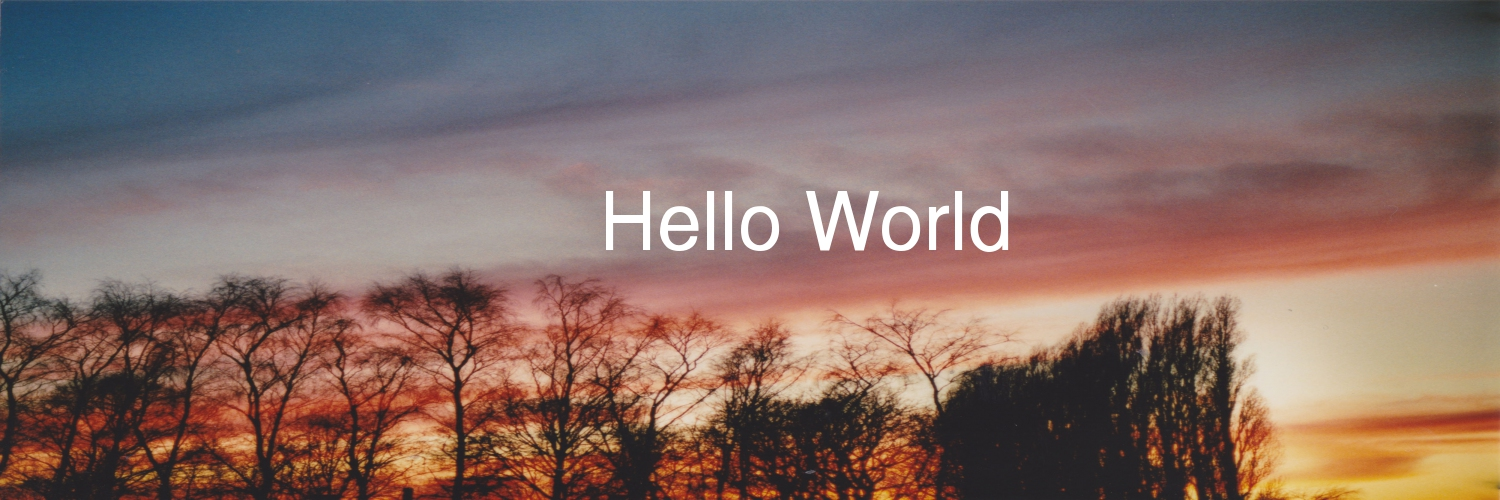
\includegraphics[width=1\textwidth]{Figuren/PHP_rendering.jpeg}
	\caption{PHP afbeelding \cite{}}
	\label{fig:PHP}
\end{figure} 
%
%https://www.thesitewizard.com/php/create-image.shtml%
%http://php.net/manual/en/book.image.php
%http://php.net/manual/en/ref.image.php
%http://jaguar.readthedocs.io/en/v1.0.0/usage/Canvas.html
%https://zinoui.com/docs/canvas

E\'{e}n van de nadelen bij het gebruik van PHP is dat het object, dat ge\"{e}xporteerd wordt door de frontend, niet rechtstreeks omgezet kan worden. Ieder object in het ge\"{e}xporteerde canvas moet overlopen worden en met de juiste eigenschappen op de afbeelding geplaatst worden. Zo moet voor elk tekst object de lettergrootte, kleur, lettertype, gewicht en tekst uit de JSON representatie van het canvas gehaald worden. In het geval van een KPI moet dan ook de tekst vervangen worden. Hoewel dit perfect mogelijk is, is het niet erg efficient en zelfs wat omslachtig. Ook kan het voorkomen dat bepaalde eigenschappen niet ondersteund of anders ge\"{i}mplementeerd zijn. 

\subsection{Node.js} \label{BackendImplementationNodeJS}
Veel gemakkelijker is het gebruiken van Node.js. Hiermee kan in de backend gebruik gemaakt worden van JavaScript code. Dit betekend dat dezelfde bibliotheken, die gebruikt worden om in de frontend de afbeeldingen te editeren, gebruikt kunnen worden in de backend. Het merendeel van de eerder besproken JavaScript bibliotheken bezit ondersteuning voor Node.js. 

Omdat Fabric, Konva en Easel allen gebaseerd zijn op het HTML canvas element, moet ook een canvas implementatie aanwezig zijn voor Node.js. De \texttt{npm-canvas} \textit{package} is gebaseerd op Cairo, een 2D \textit{graphics} bibliotheek geschreven in C. %https://github.com/Automattic/node-canvas 
Konva, Fabric en Easel werken in een Node omgeving hetzelfde als in een frontend omgeving. Een canvas wordt aangemaakt waaraan afbeeldingen, tekst, vormen en animaties toegevoegd kunnen worden. Zowel met Fabric als met Konva is het mogelijk om geserialiseerde data, in JSON formaat, terug om te zetten in een canvas. Bij Easel moeten alle objecten in het canvas opnieuw opgebouwd worden aangezien het met deze bibliotheek niet mogelijk is om JSON data om te zetten naar een canvas. 

Het omzetten van een JSON data naar een afbeelding gebeurt als volgt:
\textbf{Fabric.js}
\begin{lstlisting}[language=javascript]
	var fabric = require('fabric').fabric;
	var fs = require('fs');
	var json = {...};
	
	var canvas = fabric.createCanvasForNode(1500, 500);
	canvas.loadFromJSON(json, function() {
		canvas.renderAll();
	});
	
	var stream = canvas.createPNGStream();
	
	var out = fs.createWriteStream(__dirname + '/test-' + service + '.png');
\end{lstlisting}

Zoals te zien in de voorbeeldcode bezit Fabric methodes specifiek voor gebruik met Node.js. De \texttt{createCanvasForNode()} methode maakt een canvas aan zonder dat hiervoor een HTML canvas element nodig is. De \texttt{createPNGStream()} functie geeft een Node Stream object terug, waarmee het canvas opgeslagen kan worden als een PNG bestand. Het Stream object kan ook de data teruggeven in een base64 formaat. Aangezien dit eenvoudigweg een tekstuele representatie van binaire data is, is dit uitermate geschikt voor dit project. Wordt een Node.js service opgezet, die als input JSON data verwacht. Dan kan de \textit{response} de base64 ge\"{e}ncodeerde afbeelding bevatten. Zo wordt het mogelijk om de afbeelding bijvoorbeeld naar Facebook of Twitter te uploaden. 
%THIS IS ALSO EXPLAINED IN PRAKTISCHE UITVOERING!!! MISSCHIEN ERGENS WEGHALEN???!!!

%https://nodejs.org/api/stream.html

\textbf{Konva.js}
\begin{lstlisting}[language=javascript]
	var konva = require('konva');
	var json = {...};
	var stage = Konva.Node.create(json);
	
	stage.toDataUrl({
		callback: function(data){
			// Convert image data to png or base64 
		}
	})
\end{lstlisting} %https://github.com/konvajs/konva/blob/master/resources/nodejs-demo.js
Konva bezit geen extra methodes voor gebruik met Node.js. Maar de container parameter kan weggelaten worden bij het cre\"{e}ren van de stage aangezien er geen DOM elementen aanwezig zijn. Met behulp van de \texttt{Konva.Node.create()} methode kan JSON data omgezet worden naar een stage/canvas. Daarna kan de stage ge\"{e}xproteerd worden naar een PNG bestand of in base64 formaat met behulp van \texttt{toDataUrl()}. 

\iffalse
\textbf{Easel.js} 
Hoewel voor Easel een node-wrapper beschikbaar is %https://github.com/CreateJS/EaselJS-NodeJS
, bezit deze verre van de gewenste functionaliteit. Easel bezit geen methodes om JSON data te exporteren of importeren wat het dus moeilijk maakt om een canvas eenvoudig op te slaan voor later gebruik. Zoals eerder vermeld (zie sectie \ref{easeljs}) kan een canvas in Easel opgeslagen worden door alle objecten binnen dit canvas te overlopen en naar een JSON object om te zetten. Het inlezen gebeurt op gelijkaardige manier. Voor elk ingelezen object wordt het corresponderende object aangemaakt in de stage/canvas. Het is duidelijk dat deze manier van werken om veel meer code vraagt en omslachtiger is dan bij de andere bibliotheken.  
\fi

%https://www.taaltelefoon.be
%http://woordenlijst.org/#/?q=hoek
\subsection{Online plaatsen van de service}
% Docker (mss Jenkins ook fzo?)
Zoals eerder vermeld zal een microservice gebruikt worden om de afbeeldingen te genereren. Logischerwijze moet deze service op een server draaien zodat deze vanuit de backend, die hoofdzakelijk in PHP geschreven is, aanspreekbaar is. Om het deployen van de service gemakkelijker te maken, wordt gebruik gemaakt van Docker. 

Docker is een \textit{open-source} project gebaseerd op containers. Dit betekend dat software in ge\"{i}soleerde omgevingen zal draaien. In deze containers kunnen ontwikkelaars een applicatie opstellen met alle nodige bibliotheken en \textit{dependencies}. Containers kunnen dan op eender welk systeem ingezet worden en zullen overal hetzelfde functioneren. In tegenstelling tot Virtuele Machines (VM) bevat een container geen volledig besturingssysteem maar enkel wat nodig is om de software te doen werken. De containers delen namelijk dezelfde kernel en zullen enkel de onderdelen installeren die nog niet aanwezig zijn. Deze containers kunnen bijgevolg zeer eenvoudig gedeeld worden tussen ontwikkelaars onderling \cite{DockerWhatDocker}. 

Zoals te zien op Figuur \ref{fig:DockerDiagram} is het verschil tussen VM's en Docker duidelijk. Traditionele VM's vereisen elk een volleidg besturingssysteem wat er voor zorgt dat ze volledig afzonderlijk van hun \textit{host} functioneren. Een \textit{hypervisor} staat in voor het beheer van de VM's. Wordt Docker gebruikt, dan zorgt de lightgewicht Docker Engine voor het beheer van alle containers \cite{OpenSourceWhatDocker}. Het is duidelijk dat dit systeem het zeer eenvoudig maakt op applicaties op te zetten en te testen. Een container kan opgezet worden in enkele seconden terwijl dit bij een VM meerdere minuten duurt. Ook kunnen meer containers op \'{e}\'{e}n server geplaatst worden aangezien niet telkens een besturingssysteem ge\"{i}nstalleerd moet worden. 

\begin{figure}[H]
	\centering
	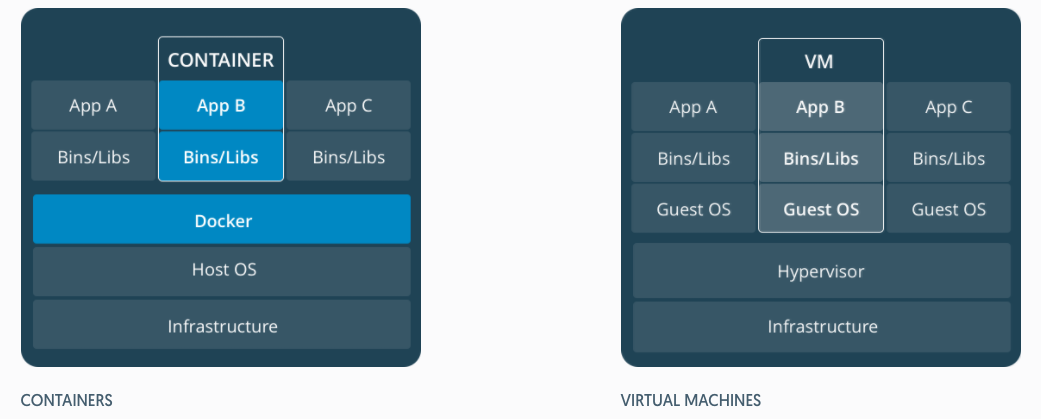
\includegraphics[width=1\textwidth]{Figuren/DockerDiagram.png}
	\caption{Docker versus VM \cite{DockerDiagram}}
	\label{fig:DockerDiagram}
\end{figure}
%http://www.teckstory.com/hadoop-infrastructure/docker-tutorial-for-beginners/
%https://devops.com/docker-vs-vms/
%MOET HIER NOG IETS BIJ???

\newpage
\section{Base64}
Dit project steunt op het bewerken van afbeeldingen. Zowel het genereren van de afbeelding in de backend als deze doorsturen naar sociale media vereist het 'transporteren' van deze afbeeldingen. Natuurlijk zou het mogelijk zijn om elke afbeelding op te slaan op de \textit{fileserver}, maar al snel zou duidelijk zijn dat dit niet de beste oplossing is. Het is namelijk de bedoeling dat een omslagfoto gegenereerd wordt met aangepaste KPI's om de zoveel tijd. Dit betekend dat iedere dag tientallen foto's aangemaakt zullen worden voor \'{e}\'{e}n profiel. Hoewel afbeeldingen gecomprimeerd kunnen worden tot enkele kilobytes, is dit toch niet de beste oplossing. Ideaal is een manier om een afbeelding door te sturen als tekst. En dit is precies wat base64 encodering mogelijk maakt. 

Base64 is een encoderingsproces die binaire data omvormt naar ASCII karakters. %Het omvormen van de data is nodig omdat binaire data \textit{null} karakters kan bevatten. De meeste applicaties zullen deze \textit{null} interpreteren als het einde van de doorgestuurde tekst. 
In principe worden simpelweg drie octetten omgezet in vier ge\"{e}ncodeerde karakters. Tijdens het encoderen wordt de binaire data gesplitst in groepjes drie bytes. Deze groepen bestaan dan uit vier groepen van zes bits (2\textsuperscript{6} = 64 karakters). Deze zes bits worden met behulp van de base64 encoderingstabel (zie Figuur \ref{fig:Base64Table}) omgezet in ASCII karakters \ref{Base64}. Wanneer de laatste groep niet genoeg bytes bevat om een 6-bit karakter op te stellen, kan \textit{padding} toegevoegd worden. In de binaire data vertaald dit zich in het toevoegen van nullen op het eind tot een 6-bit karakter gevormd wordt. In de ASCII tekst wordt deze padding voorgesteld door een '='. Een voorbeeld van het volledige proces is hier te zien: 
%MSS laatste zin weg doen en ref naar afbeelding fzo? idk

\begin{figure}[H]
	\centering
	\includegraphics[width=1\textwidth]{Figuren/Base64Process.png}
%	\caption{Base64 omzetting}
	\label{fig:Base64Table}
\end{figure}

\begin{figure}[H]
	\centering
	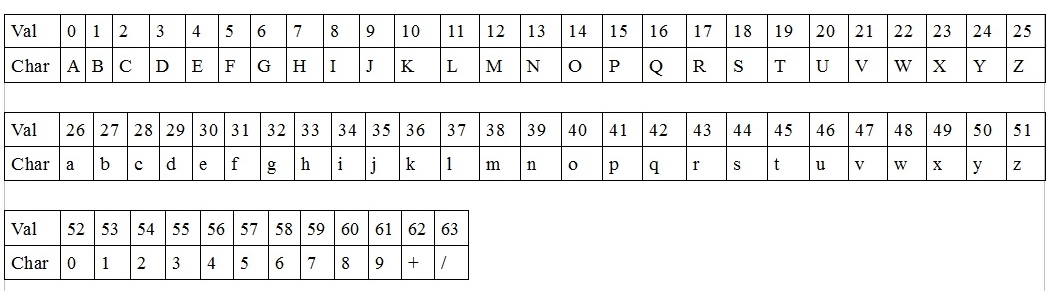
\includegraphics[width=0.7\textwidth]{Figuren/Base64EncodingTable.jpg}
	\caption{Base64 encoding tabel \cite{Base64Image}}
	\label{fig:Base64Table}
\end{figure} 

%maybe: https://www.youtube.com/watch?v=29Nd_sr6GYU
Wordt de volledige stream van binaire data op deze manier ge\"{e}ncodeerd, wordt uiteindelijk \'{e}\'{e}n lange \textit{string} bekomen die verstuurd kan worden in een \textit{response} of \textit{request}.

\iffalse
\newpage
\section{Functioneel ontwerp}
Bij het implementeren van een nieuwe \textit{feature} is het logisch dat hiervan vooraf een ontwerp gemaakt wordt. Hoewel het ontwerpen een iteratief proces is, 
\textit{profile manager} 


\begin{figure}[H]
	\centering
	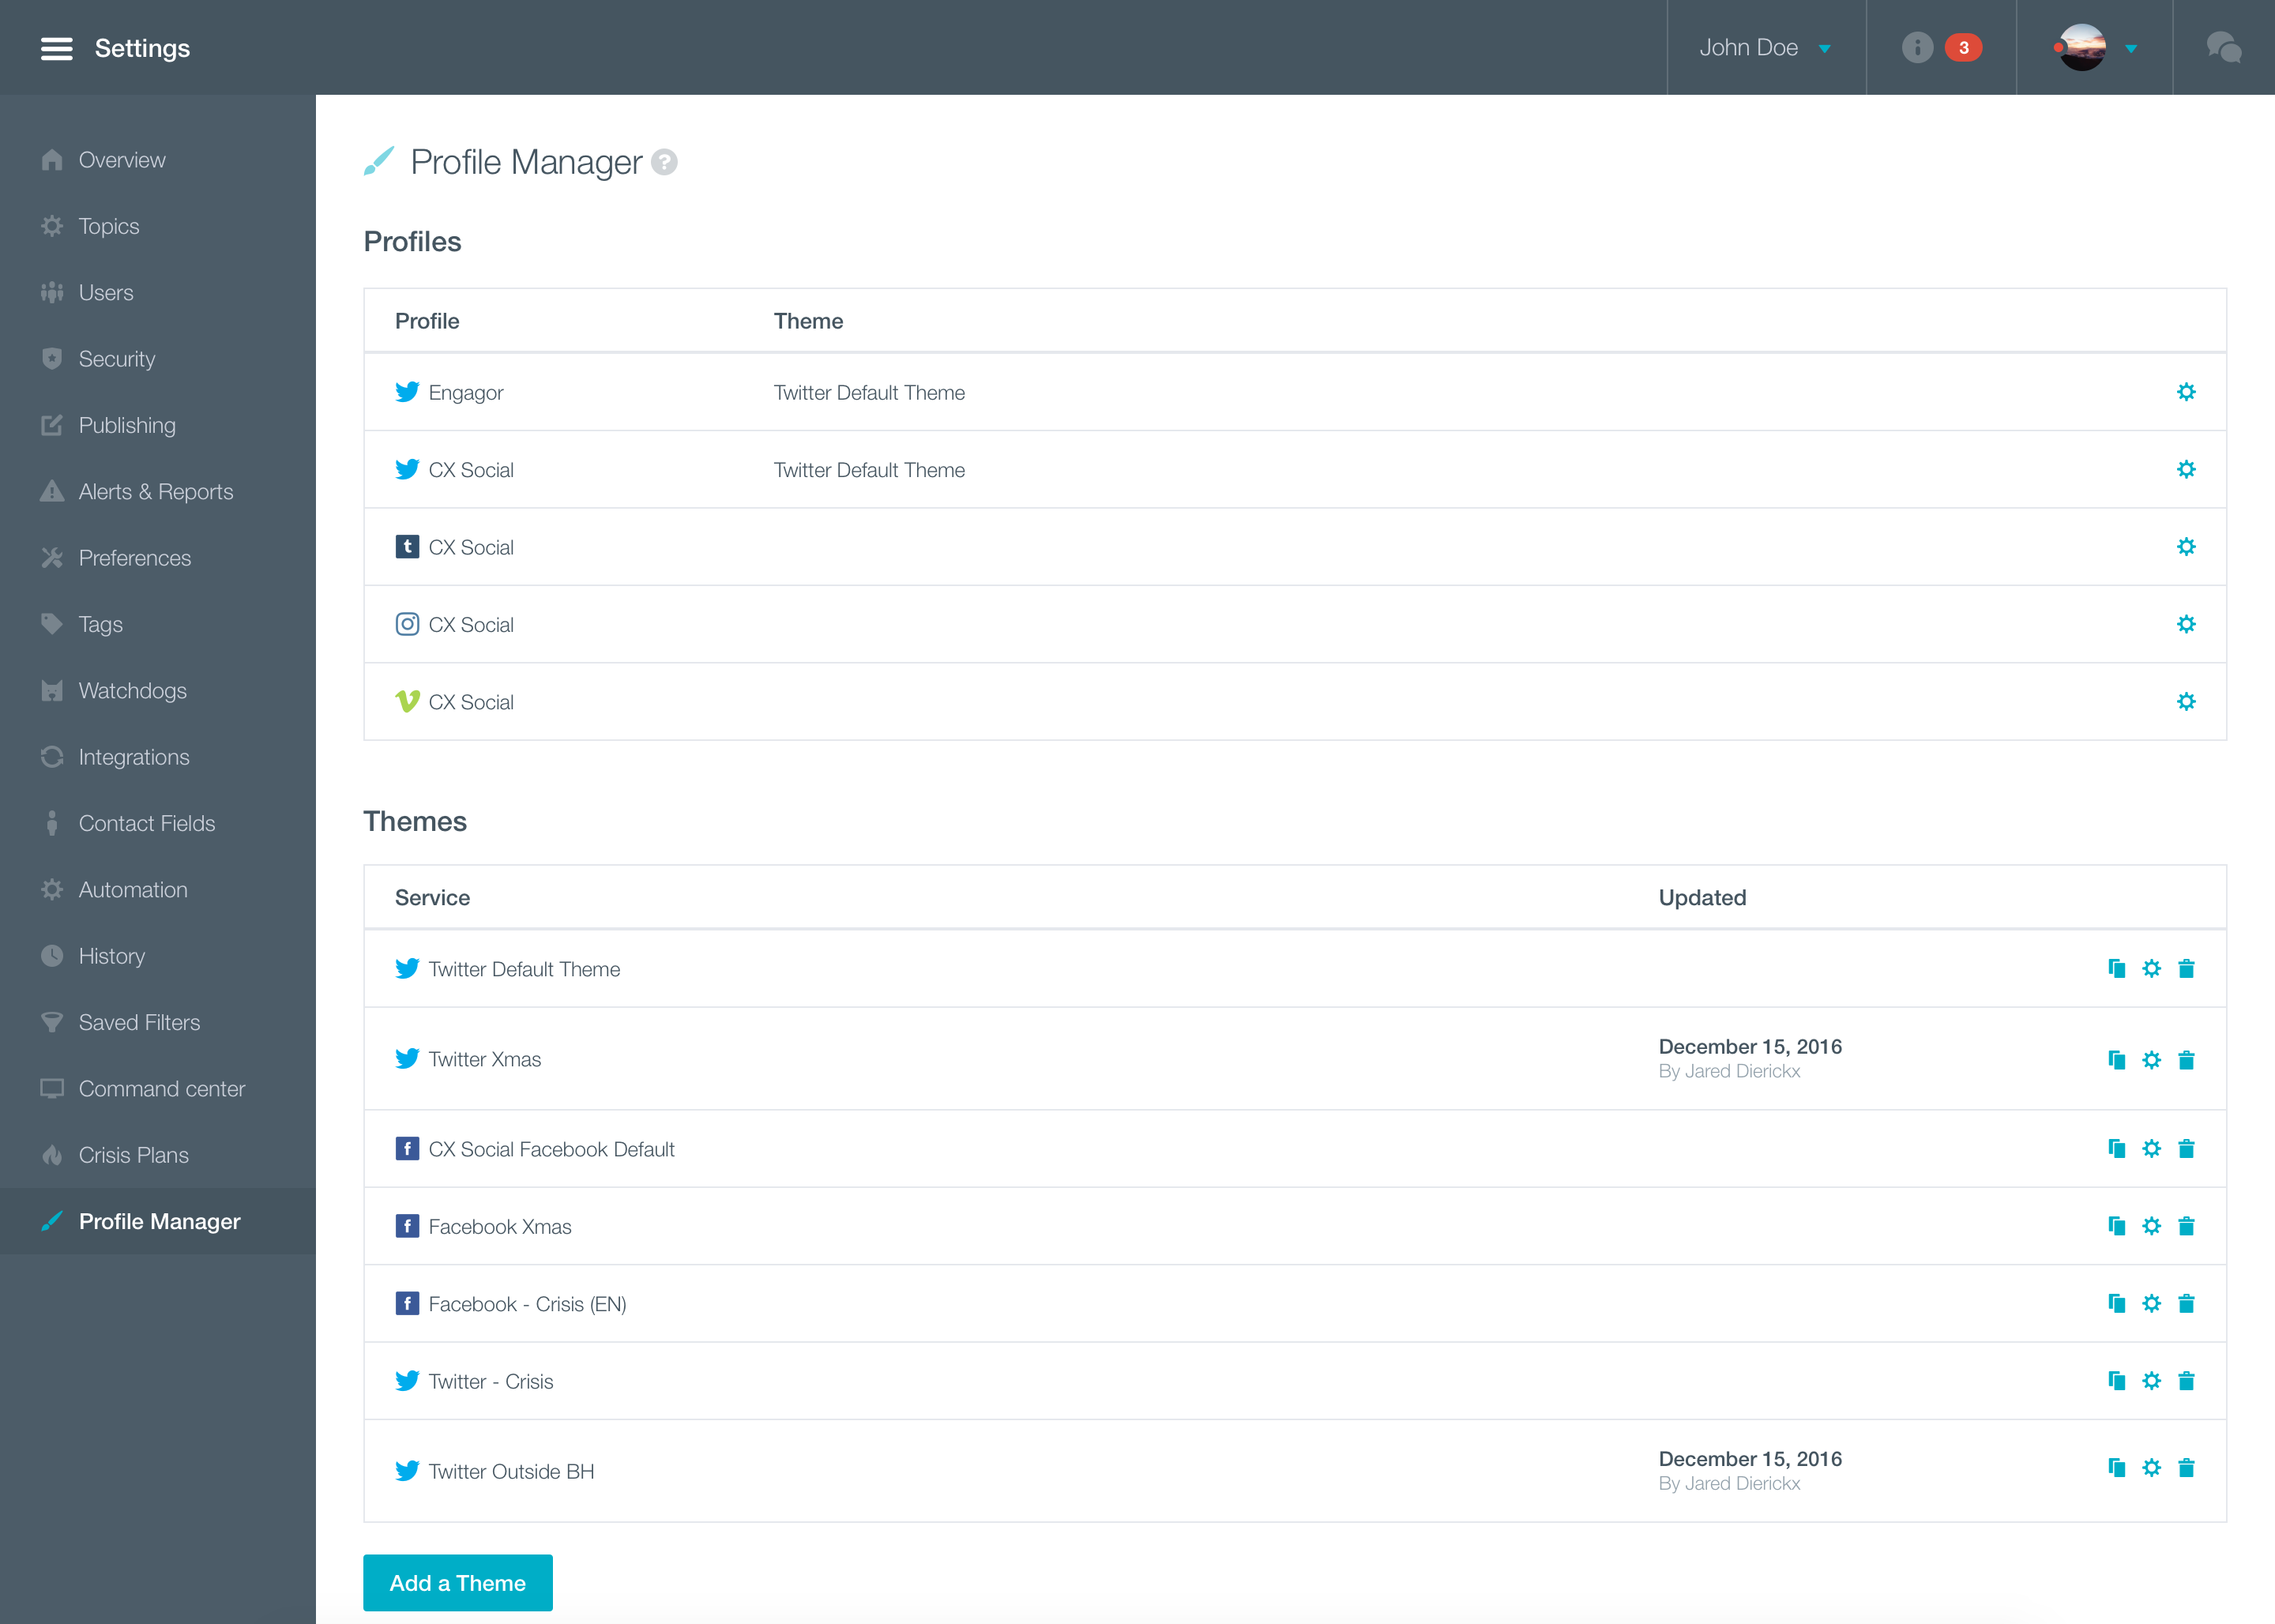
\includegraphics[width=0.7\textwidth]{Figuren/Mockups/Overview.png}
	\caption{Profile Manager Overview}
	%\label{fig:Base64Table}
\end{figure} 

\begin{figure}[H]
	\centering
	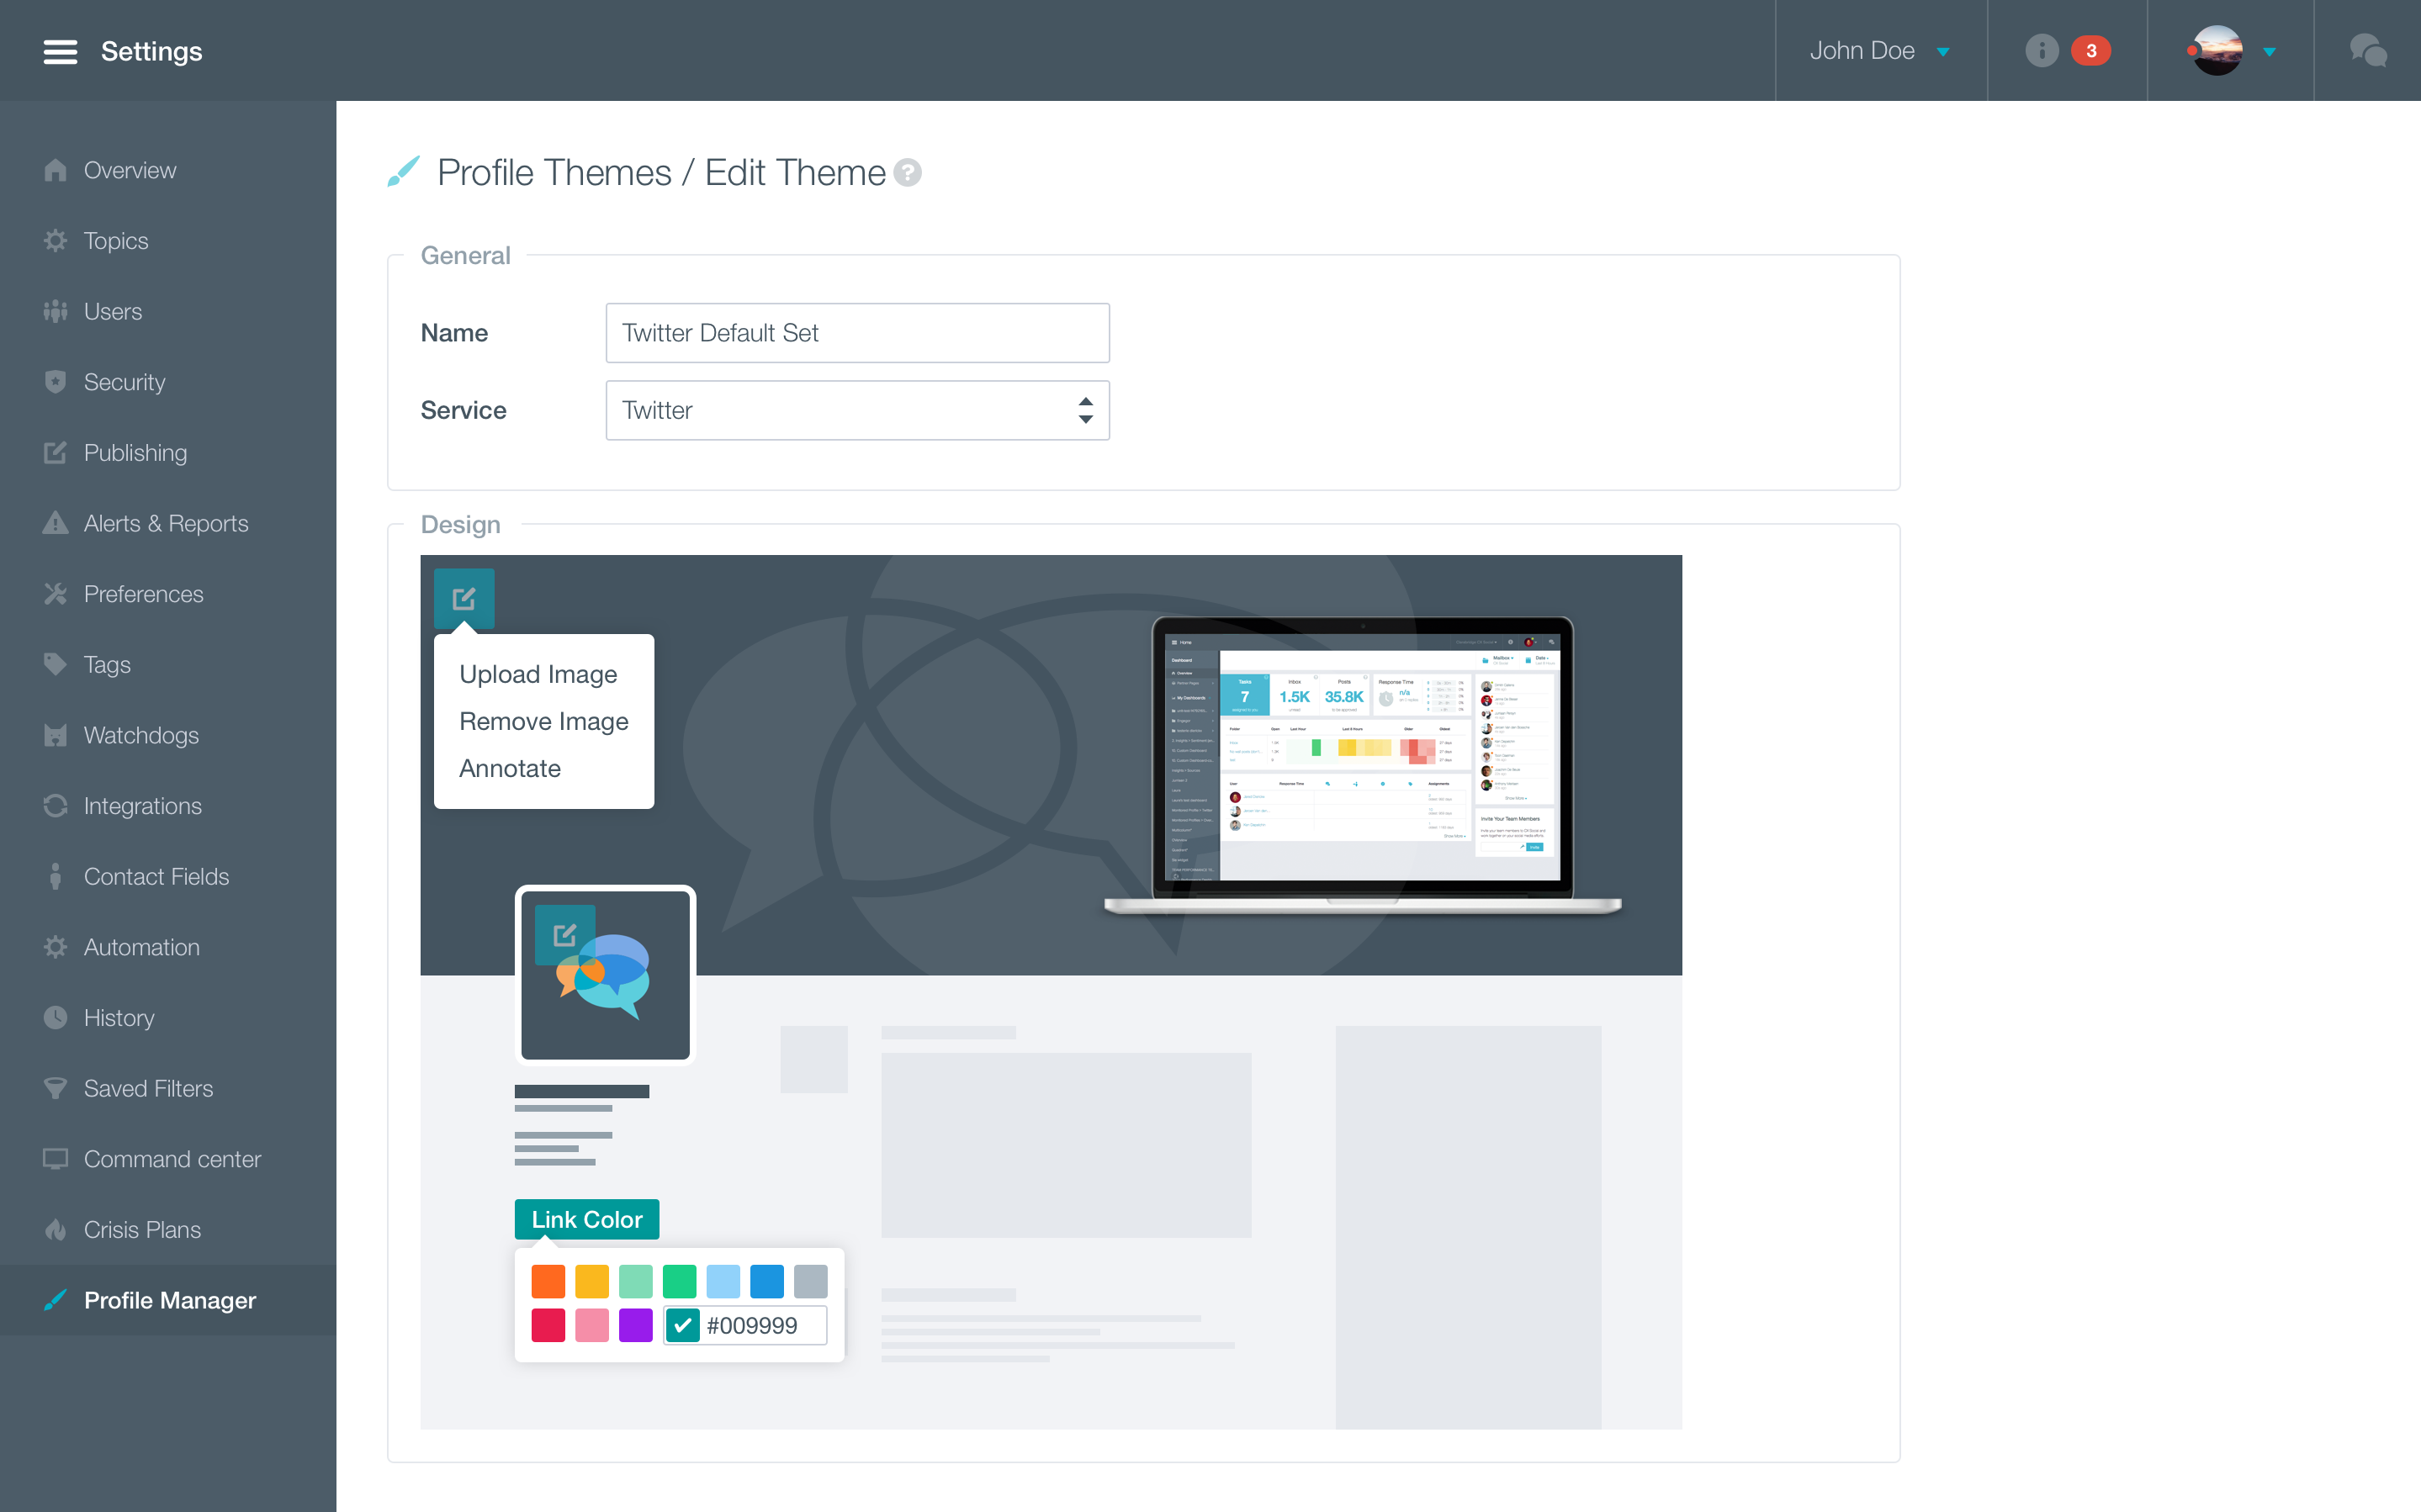
\includegraphics[width=0.7\textwidth]{Figuren/Mockups/AddTheme.png}
	\caption{Profile Manager Overview}
	%\label{fig:Base64Table}
\end{figure} 

\begin{figure}[H]
	\centering
	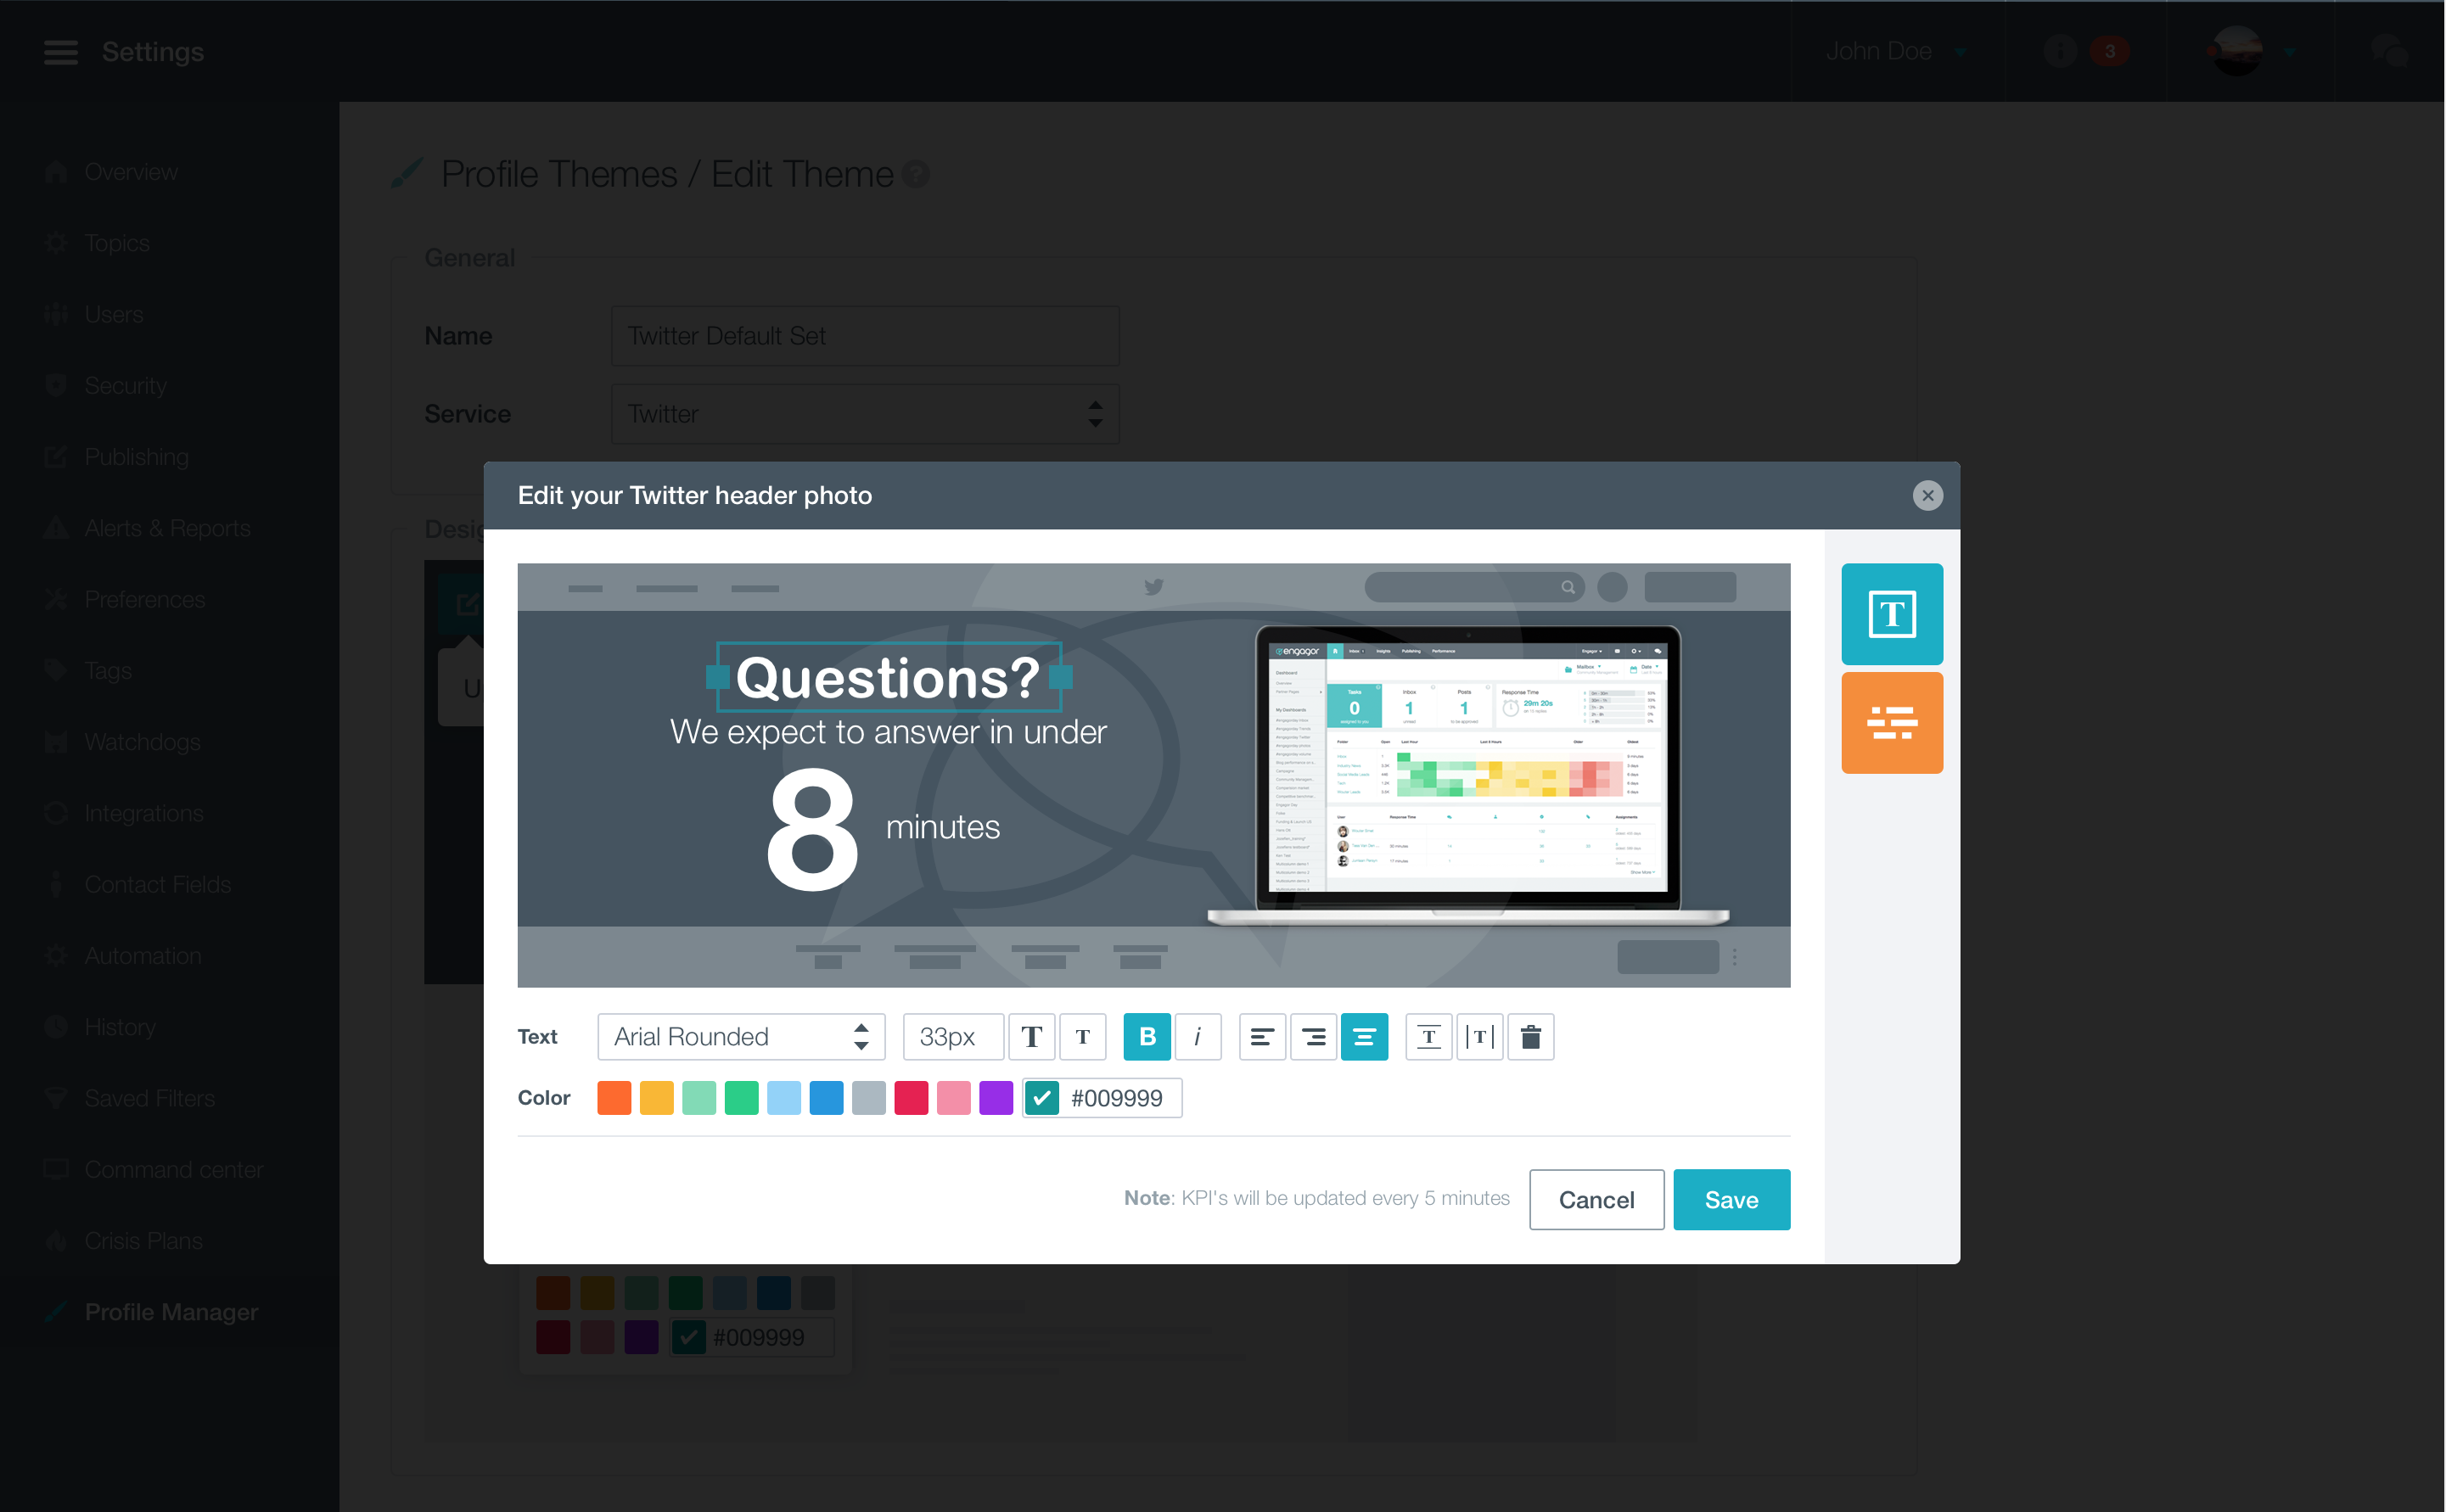
\includegraphics[width=0.7\textwidth]{Figuren/Mockups/AnnotationsDialog.png}
	\caption{Profile Manager Overview}
	%\label{fig:Base64Table}
\end{figure} 

\begin{figure}[H]
	\centering
	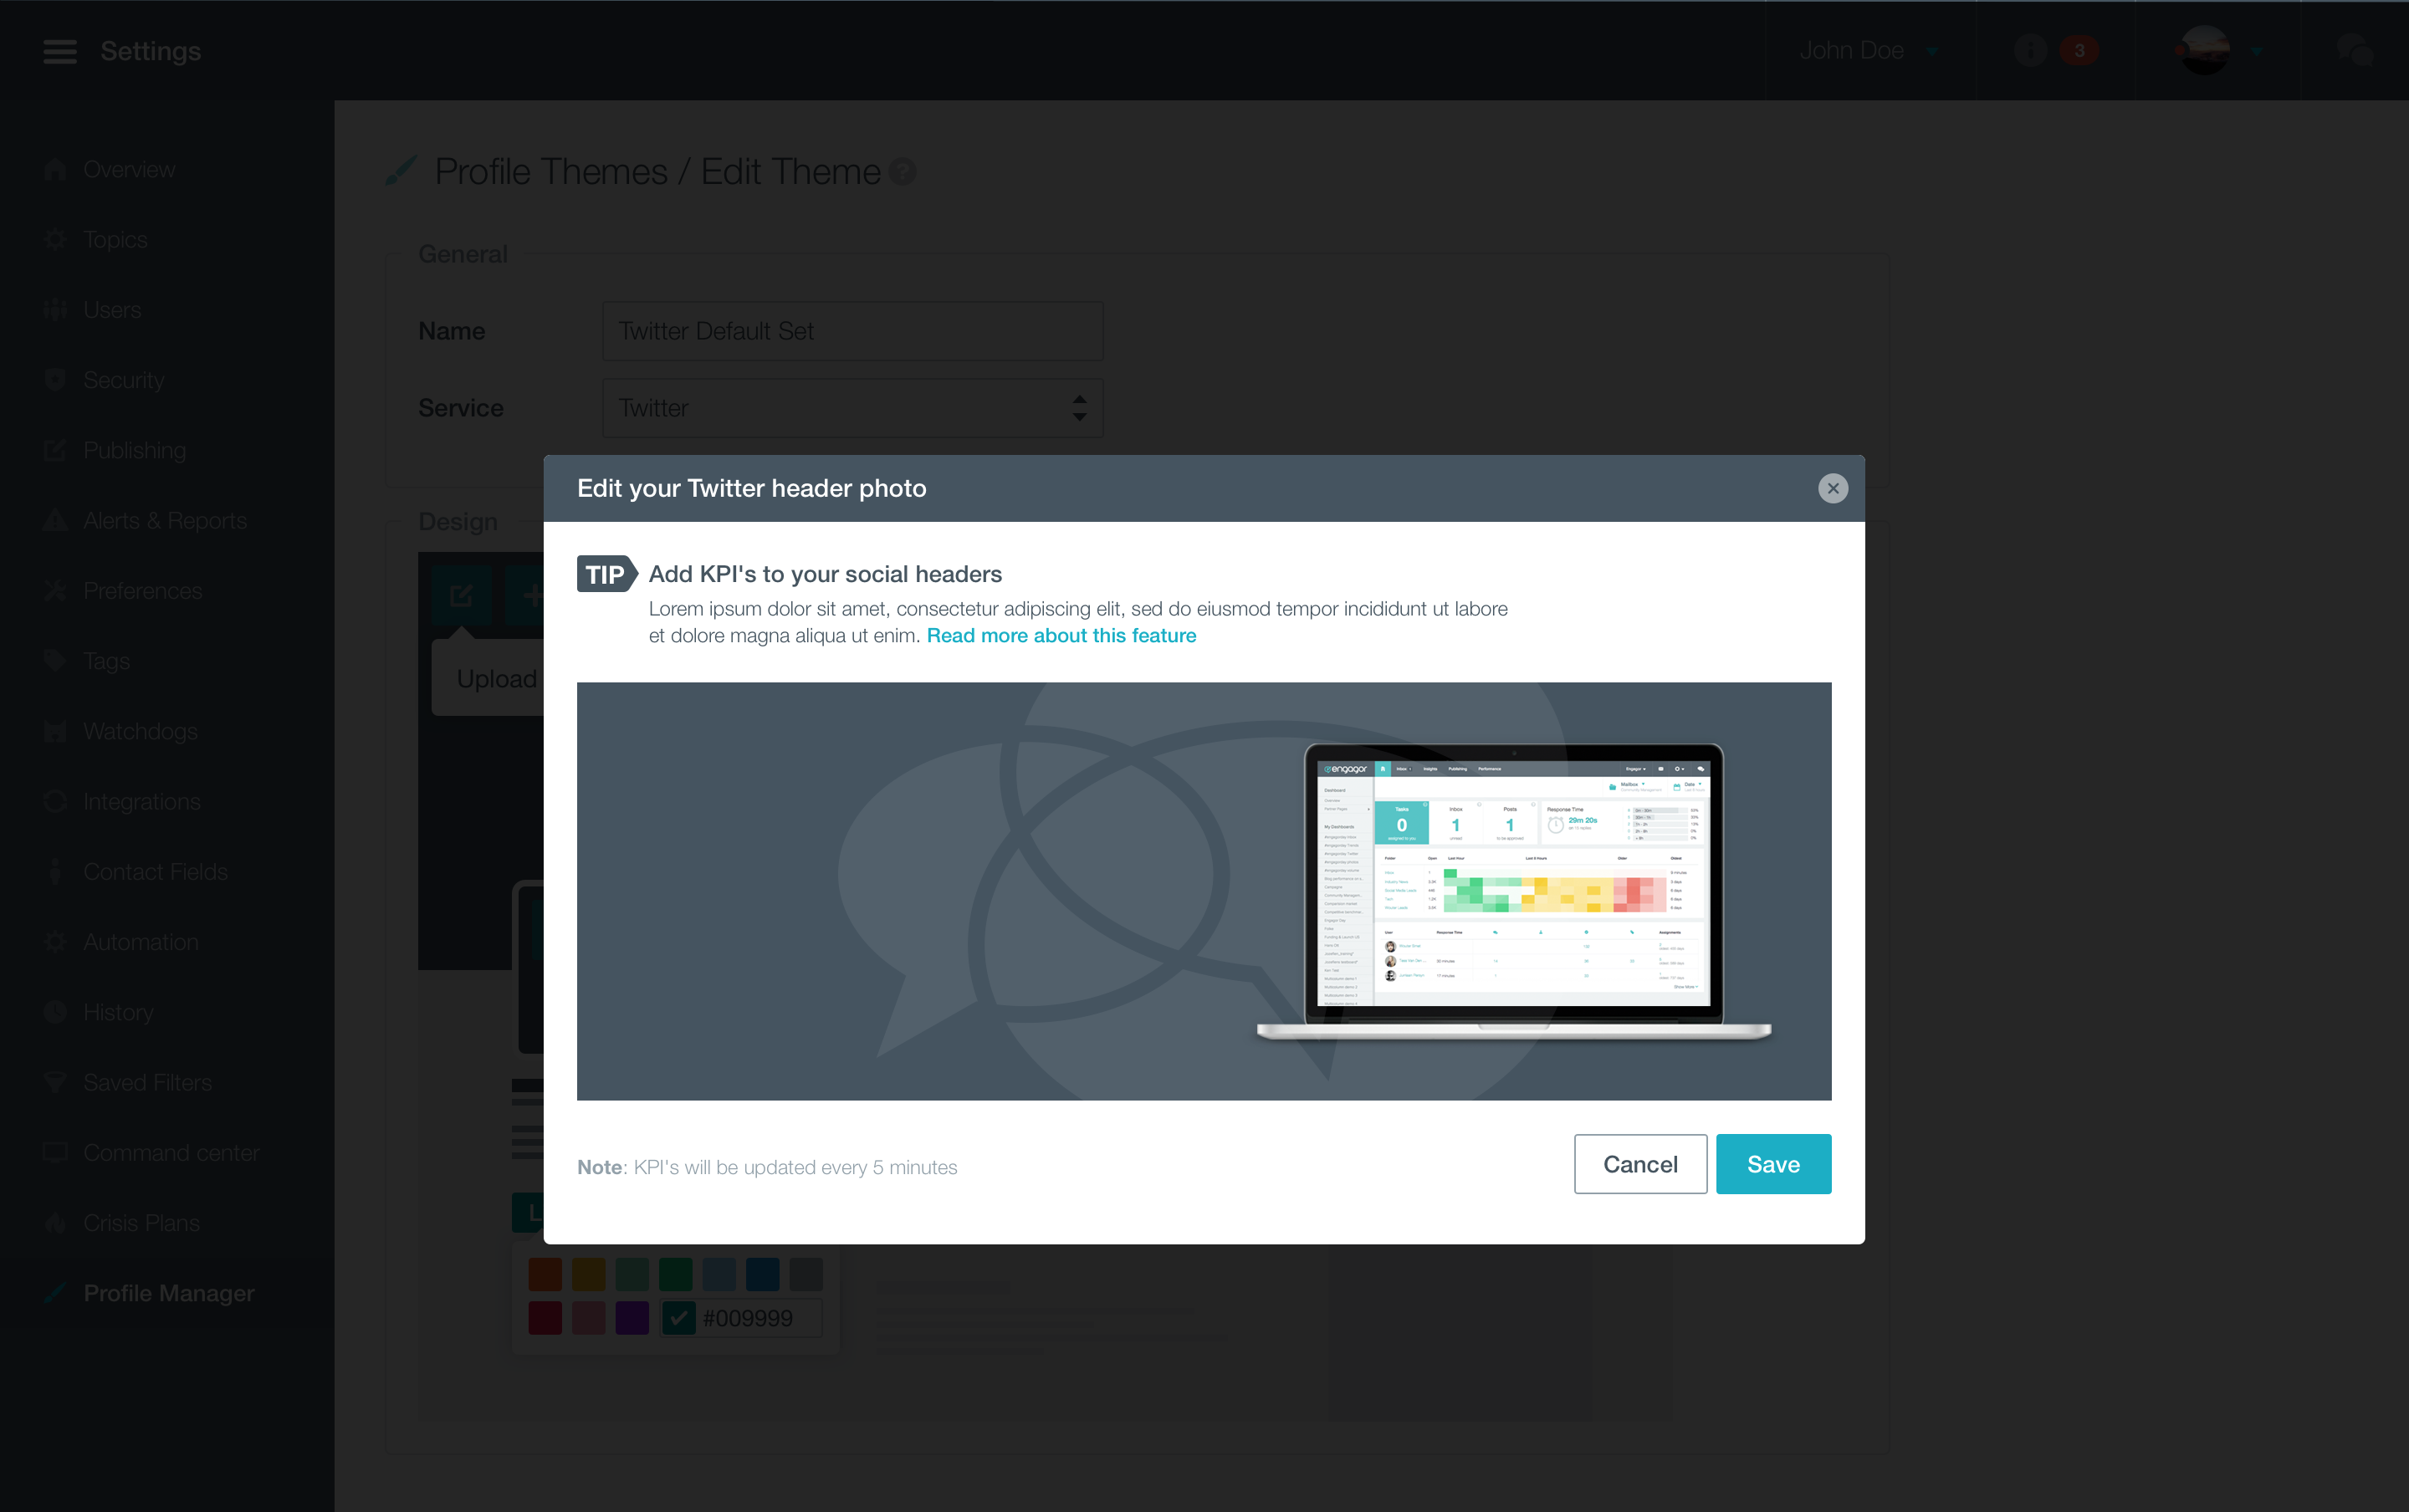
\includegraphics[width=0.7\textwidth]{Figuren/Mockups/EditDialog.png}
	\caption{Profile Manager Overview}
	%\label{fig:Base64Table}
\end{figure} 

\begin{figure}[H]
	\centering
	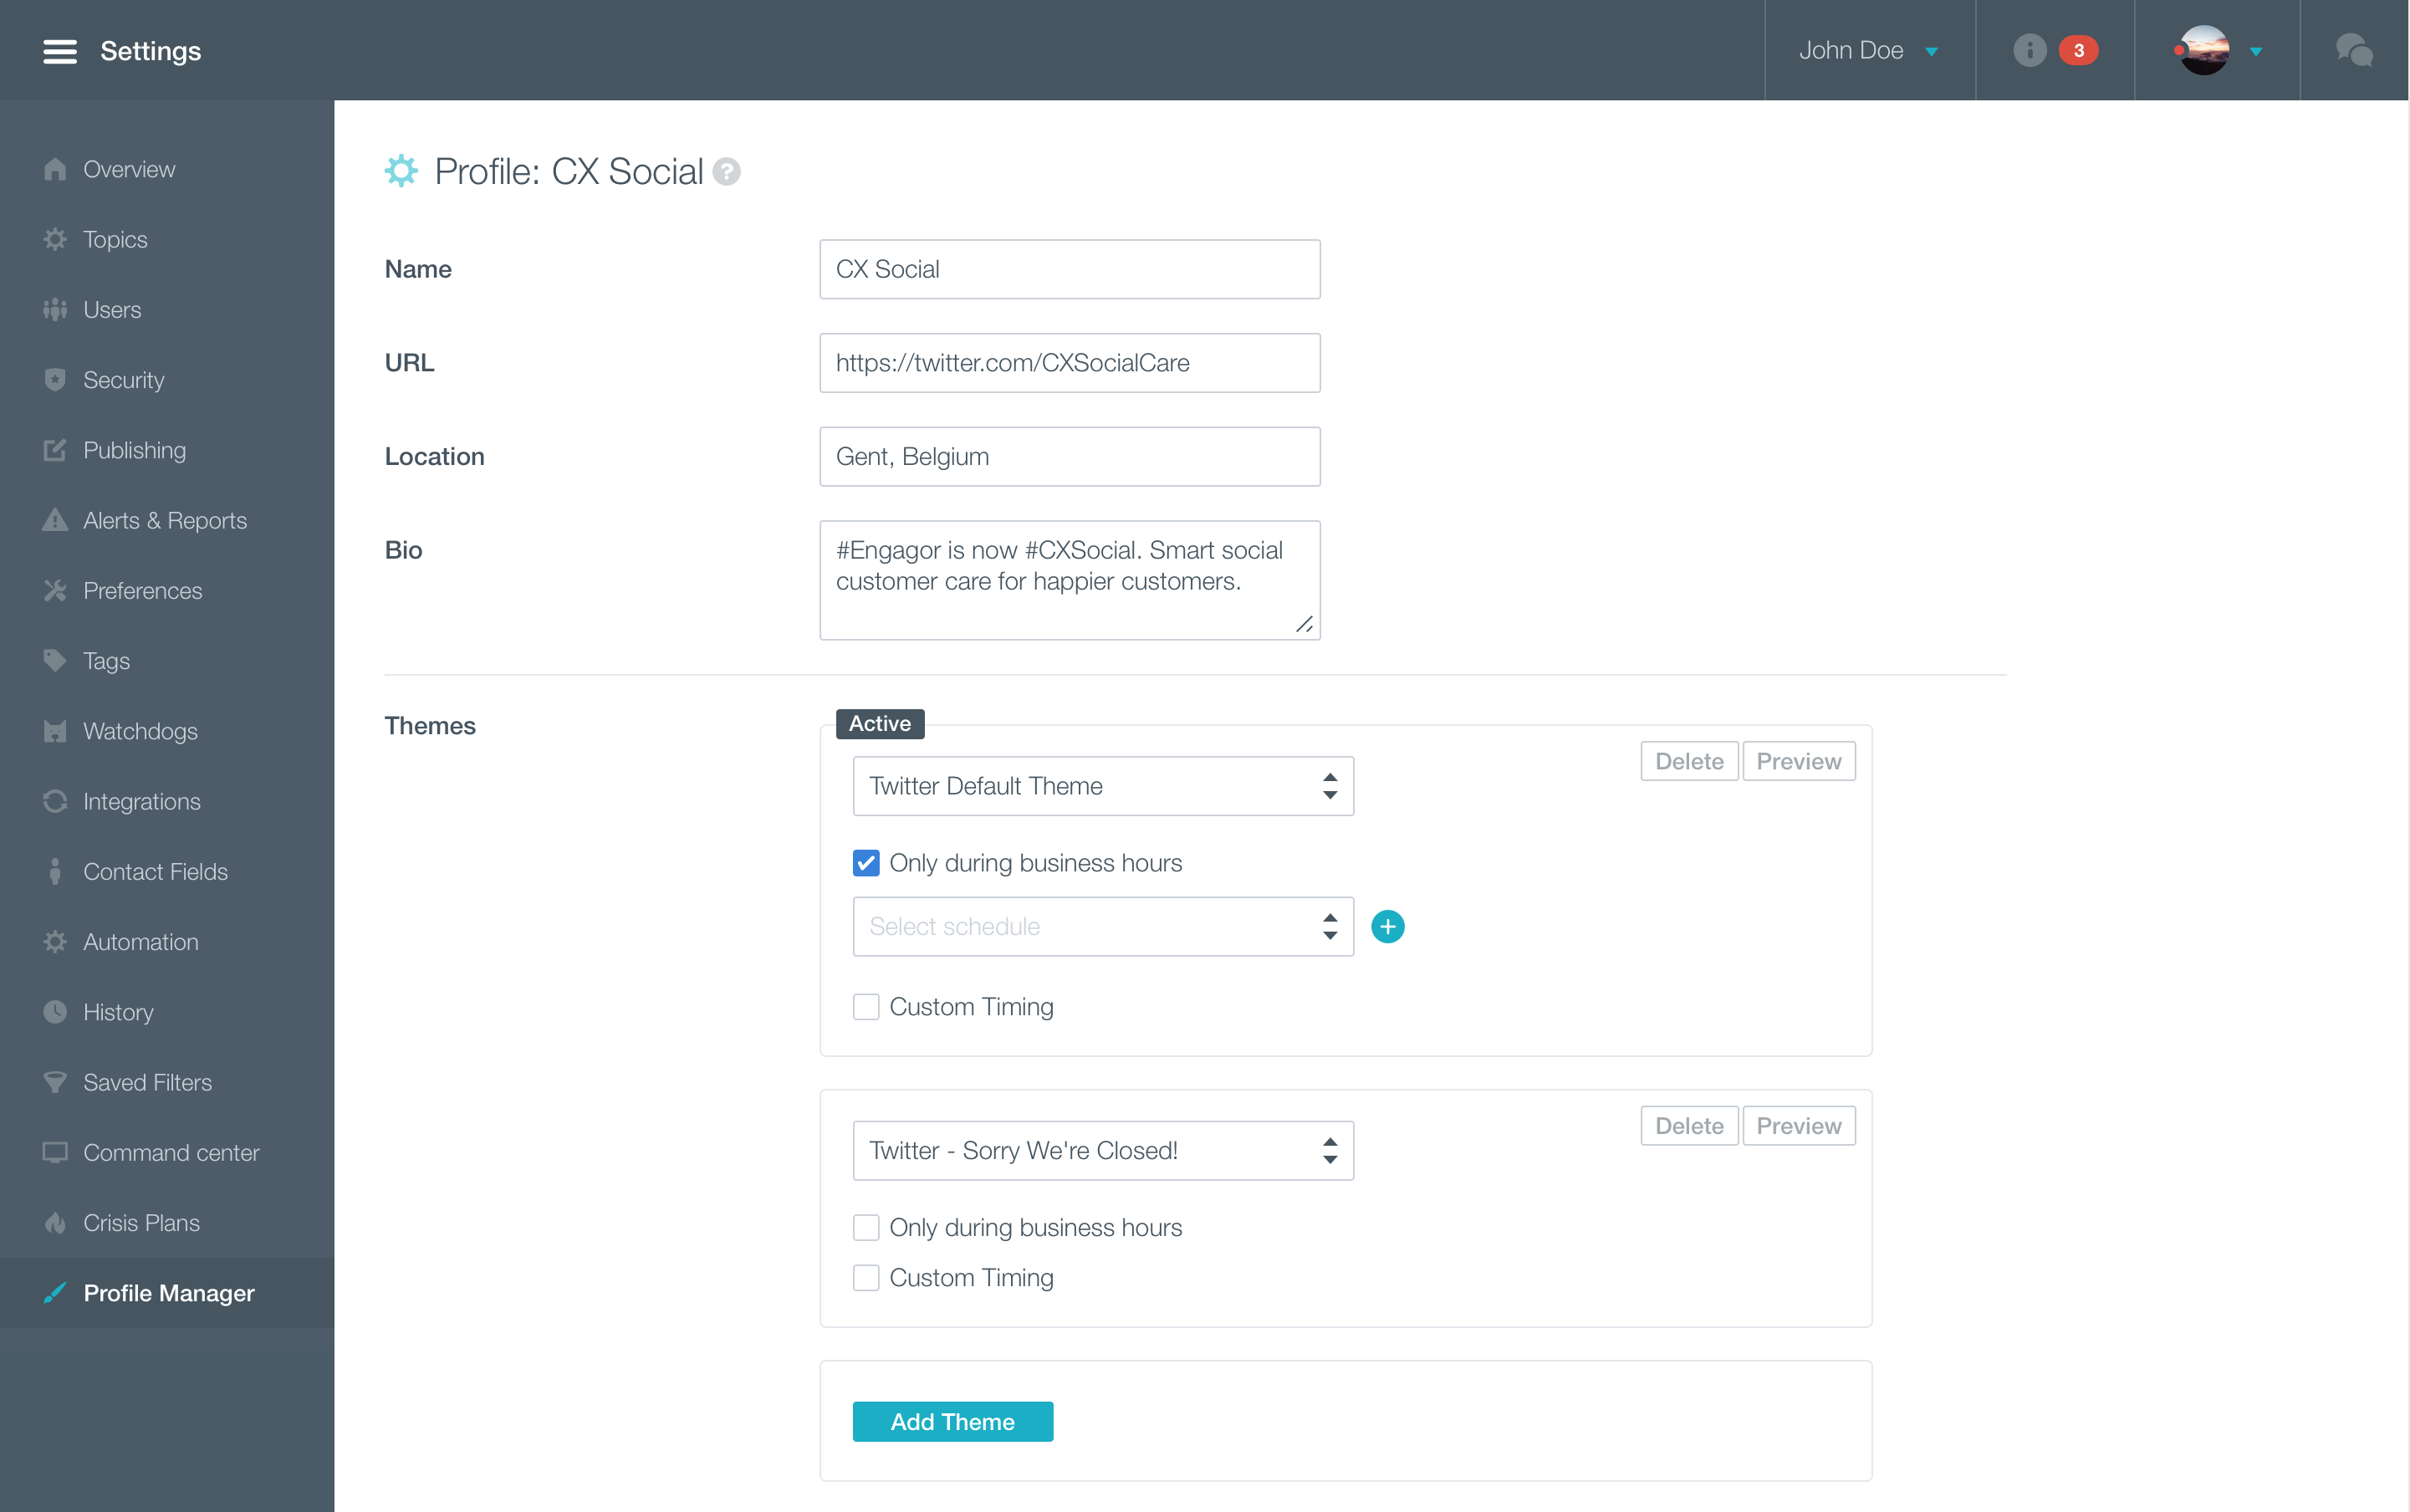
\includegraphics[width=0.7\textwidth]{Figuren/Mockups/EditProfile.png}
	\caption{Profile Manager Overview}
	%\label{fig:Base64Table}
\end{figure} 
\fi








%\section{Afbeelding compressie}




%
%\begin{table}[ht!]
%\begin{center}
%\begin{tabular}[c]{clllc}
%\hline
%Schaalwaarde & Product & Merk of soort & Staalgrootte & Temperatuur\\
%\hline
%1 & Roomkaas & Kraft Philadelphia & 1.5 cm\textsuperscript{2} & 7-13\degree~C\\
%2 & Wit van ei & Hardgekookt(5 min.) & Tipje van 1.5 cm &	20-25\degree~C\\
%3	& Frankfurterworst &	Schneiders, groot	& Sneetje van 1.5 cm	& 10-18\degree~C\\
%4	& Kaas &	Kraft mild Cheddar & 1.5 cm\textsuperscript{2} & 10-18\degree~C\\
%5	& Olijven	& McLaren's, gevuld	& 1 olijf zonder pit &	10-18\degree~C\\
%6	& Pindanoten	& Cocktail-type &	1 noot & 20-25\degree~C\\
%7	& Wortelen	& Ongekookt, vers	& Sneetje van 1.5 cm	& 20-25\degree~C\\
%8	& Amandelen	& McNair, geblancheerd &	1 noot	& 20-25\degree~C\\
%9	& Pepermuntbal	& McCormick	& 1	& 20-25\degree~C\\
%\hline
%\end{tabular}
%\caption{Voorbeeld hardheidsschaal. Naar Szczesniak (1963)} % hade moet bron nog vermelden
%\label{tabeltextureprofiling}
%\end{center}
%\end{table} 
%
%\begin{figure}[ht!]
	%\centering
		%\includegraphics[width=0.50\textwidth]{Figuren/Kwantitatievedescriptieveanalyse.pdf}
		%\caption{Voorbeeld van een kwantitatieve descriptieve analyse tussen product A en product B, twee soorten sinaasappelgelei. Naar \cite{lawless2010sensory}}
	%\label{fig:Kwantitatievedescriptieveanalyse}
%\end{figure}

% !TeX spellcheck = <Dutch>

\chapter{\textbf{Praktische uitwerking}}
\vspace{-3cm}
Het annoteren van afbeeldingen is \'{e}\'{e}n van de onderdelen binnen de \textit{Profile Manager} van CX Social. De \textit{Profile Manager} is een nieuwe feature die gebruikers moet helpen bij het beheren van hun sociale media profielen. Een thema kan aangemaakt worden voor Facebook of Twitter dat een omslag-en/of profielfoto bevat. Eens een omslagfoto ge\"{u}pload is, is het mogelijk om annotaties toe te voegen. Dit kan simpelweg tekst zijn maar ook KPI's kunnen op de afbeelding geplaatst worden. Gebruikers kunnen voor geconnecteerde profielen instellen welk thema op welk tijdstip actief moet zijn. De aangemaakte afbeeldingen worden dan op de ingestelde tijdstippen ge\"{u}pload naar het juiste profiel. 


\section{Frontend implementatie}
Een groot deel van de frontend code van CX Social is geschreven met React. Met React kunnen makkelijk componenten aangemaakt worden om zo complexe interfaces aan te maken. Om de \textit{Profile Manager} zo modulair mogelijk te maken worden de verschillende \textit{features} opgesplitst in React componenten. 

\subsection{Aanmaken van een thema} \label{AanmakenVanEenThema}

 %2o zijn er heel wat componenten beschikbaar waarmee gemakkelijk functionaliteit aan een pagina kan toegevoegd worden.
Om een thema aan te maken zijn een naam, een \textit{service} %CHECK IF ITS ITALIC EVERYWHERE!!! 
en twee velden nodig om afbeeldingen te uploaden (zie Figuur \ref{fig:ThemeComponent}). Aangezien dezelfde functionaliteit vereist is wanneer een thema aangepast wordt, wordt gebruik gemaakt van een React component. Deze \texttt{ThemeComponent} stelt een volledig thema voor en zal alle veranderingen hieraan afhandelen. Dit betekend dus zowel het ingeven van de naam en service als het bijhouden van de geannoteerde afbeeldingen. Uiteindelijk is het deze component die instaat voor alle interacties met een thema. 
%Zowel het aanmaken als editeren van een thema verwachten dezelfde functionaliteit.
%Eens een thema aangemaakt is, kan het later ook aangepast worden. Omdat dezelfde functionaliteit op twee verschillende pagina's nodig is, wordt hiervoor een React component aangemaakt: de \texttt{Theme} component (zie Figuur \ref{fig:ThemeComponent}). 
Bij het aanmaken van de \texttt{ThemeComponent} dienen enkele eigenschappen meegegeven te worden. Eerst en vooral wordt het, uit de databank opgehaalde, thema meegegeven indien dit beschikbaar is. %ADD SOME INFO OVER HOW IT IS IN VIEW, WHEN NO THEME IS SELECTED!

\begin{figure}[H]
	\centering
	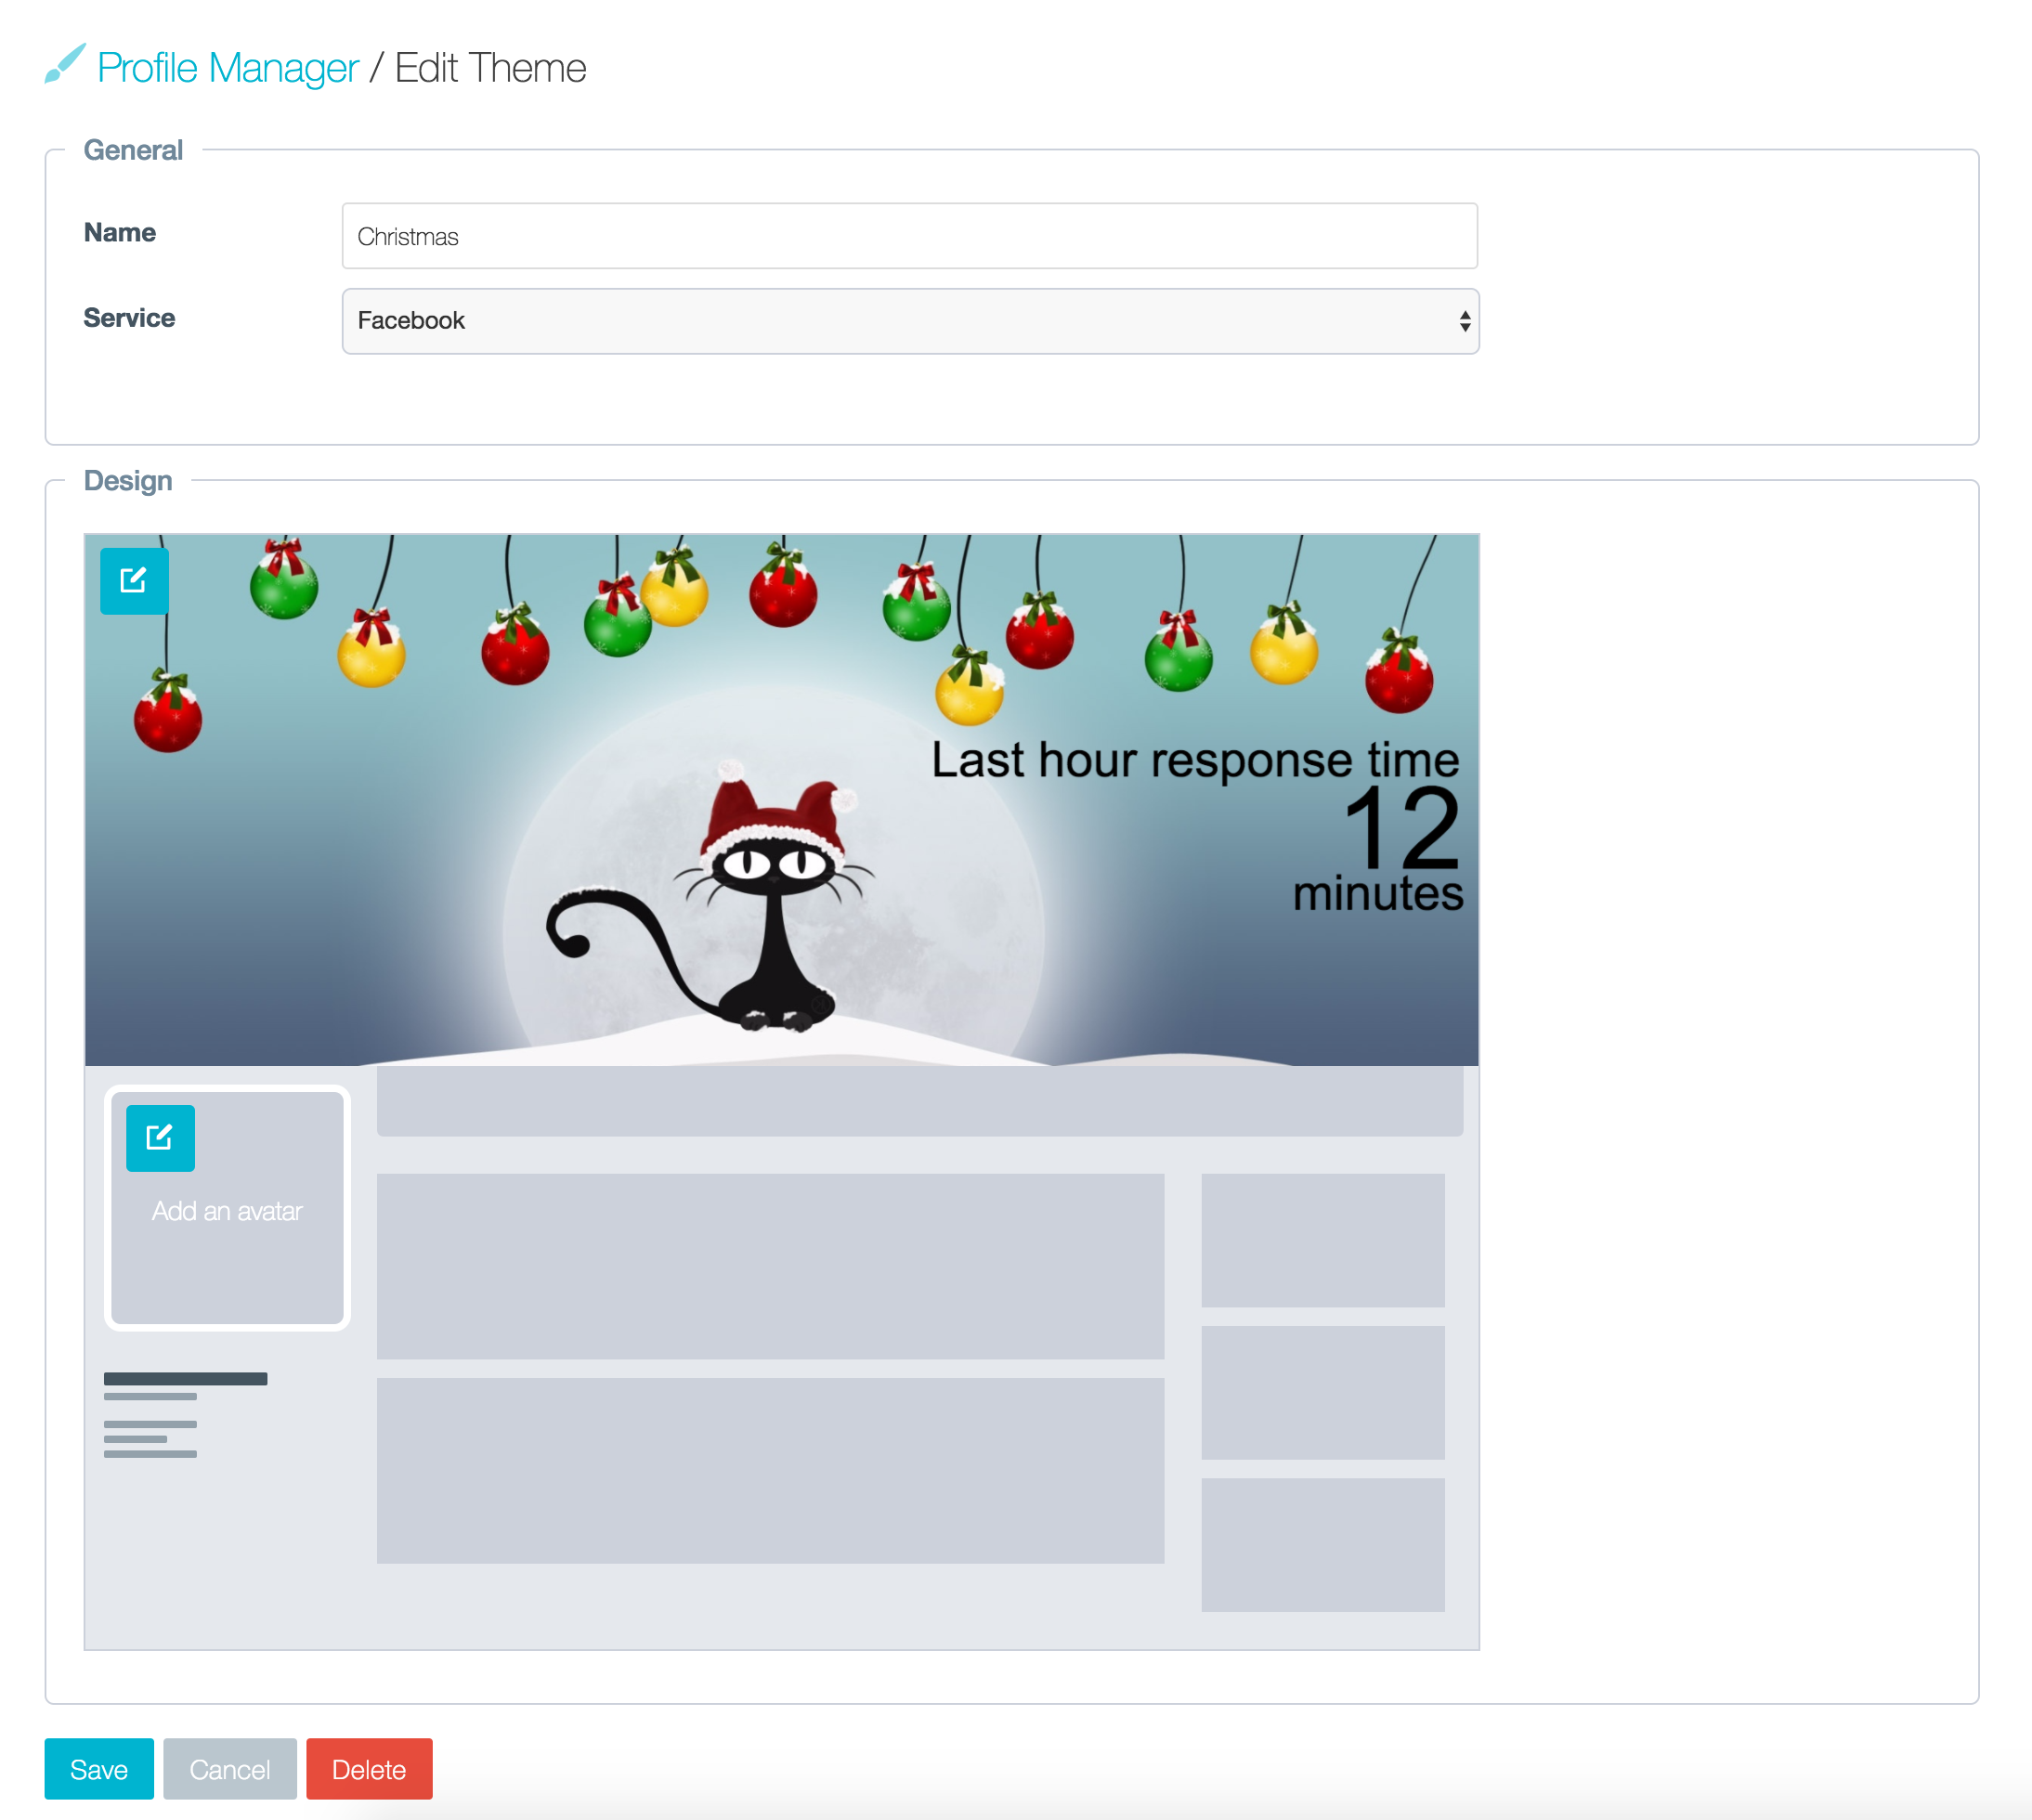
\includegraphics[width=0.6\textwidth]{Figuren/ThemeComponent.png}
	\caption{ThemeComponent in de editeer pagina}
	\label{fig:ThemeComponent}
\end{figure} 

Het account \textit{Identity Document} (ID), \textit{Cross-site requrest forgery} (CSRF) token, beschikbare services, en de annotatiepermissie zijn verplichte eigenschappen van de component. Deze eigenschappen zullen nooit veranderen tijdens de levensduur van het component, het zijn dus constanten. Het CSRF token wordt aan het formulier toegevoegd om ongeauthoriseerde acties in applicaties te voorkomen. Met het token wordt ervoor gezorgd dat geen ongeldige \textit{requests} gemaakt kunnen worden. %http://stackoverflow.com/questions/5207160/what-is-a-csrf-token-what-is-its-importance-and-how-does-it-work
Niet elke gebruiker heeft dezelfde rechten in CX Social. Binnen een bepaald plan zijn verschillende gebruikersrollen beschikbaar. Zo zijn er gewone gebruikers, \textit{admins}, managers, \textit{editors}, \textit{contributors} en \textit{analytics users}, elk met hun eigen rechten. Permissies, die aan de gebruiker werden toegekend, worden meegegeven aan de Theme component om de annoteer \textit{feature} al dan niet beschikbaar te stellen. Ieder inputveld bevat een \texttt{onChange} event waarmee veranderingen afgehandeld kunnen worden. Zoals te zien in codevoorbeeld \ref{lst:ThemeComponentDropdown} wordt de state van de component ge\"{u}pdatet wanneer een verandering aan de inputvelden plaatsvindt. De state van de component kan, in tegenstelling tot de eigenschappen (props), wel veranderen binnen het component. De state kan aangepast worden met behulp van  de \texttt{setState()} methode. 

\begin{lstlisting}[caption={Theme component - Dropdown},label=lst:ThemeComponentDropdown,language=javascript]
<select className={this.state.saving && this.state.service === '' ? 'error 		fieldset-input' : 'fieldset-input'} id="service" name="service" ref="service" value={this.getService()}
	onChange={function (event) {
		this.setState({service: event.target.value});
	}.bind(this)}>
	{this.props.services.map(function (service) {
		return <option key={service} value={service}>{this.capitalize(service)}</option>
	}.bind(this))}
</select>
\end{lstlisting}

Naast het ingeven van een naam en \textit{service} voor het thema, kunnen ook een omslag-en profielfoto toegevoegd worden. Het uploaden van de afbeeldingen wordt afgehandeld door een reeds bestaande component. Deze zal een, door de gebruiker geselecteerde, foto uploaden naar de \textit{fileserver} en op de pagina weergeven. Eens een afbeelding aanwezig is, is het mogelijk om annotaties toe te voegen. Om een afbeelding te annoteren wordt een pop-upvenster geopend. Aangezien deze pop-up een volledig nieuwe \textit{template} is, dienen enkele eigenschappen van het thema meegegeven te worden. Als parameters in de URL worden zowel de \textit{service} als de bestandsnaam van de afbeelding op de fileserver meegegeven. Beide parameters zijn nodig om het canvas op te stellen. De \textit{service} bepaald immers de dimensies van het canvas aangezien deze verschillen voor zowel Facebook als Twitter. Via de bestandsnaam kan de correcte afbeelding ingeladen worden in het pop-upvenster.

Zoals reeds besproken in sectie \ref{vergelijkingBibliotheken}, lijkt Fabric.js de beste keuze te zijn om dit project uit te werken. Aangezien niet alle functionaliteit van deze bibliotheek van toepassing zijn op dit project, wordt een \textit{custom build} aangemaakt. Deze bevat de tekst, interactieve tekst, animatie, serialisatie, interactie en node \textit{features}. Bij het openen van het pop-upvenster wordt het \texttt{ThemeAnnotations} component ge\"{i}nitialiseerd met de nodige eigenschappen. Deze zijn het account ID, de bestandsnaam van de afbeelding, de \textit{service} en een kleurenpallet. Tussen deze kleuren en eender welke hexadecimale waarde kan gekozen worden tijdens het stylen van de annotaties.

\begin{lstlisting}[caption={ThemeAnnotations component - initialisatie}\label{ThemeComponentDropdown},language=javascript]
$(document).ready(function() {
	var annotationProps = {
		accountId: '{{account.id}}',
		image: '{{image}}',
		service: '{{service}}',
		colors:  [
		"#FF691F",
		"#FAB81E",
		"#7FDBB6",
		"#19CF86"
		]};
		
	ReactRenderer.render(
		React.createElement(ThemeAnnotations, annotationProps),
		document.getElementById('annotations'),
		$.noop()
	);
});
\end{lstlisting}

\subsection{Annoteren van de afbeelding}\label{AnnoterenVanAfbeelding}
Het annoteren van een ge\"{u}ploade afbeelding vindt plaats in een  pop-upvenster. Zoals vermeld in sectie \ref{AanmakenVanEenThema}, wordt hiervoor ook een React component aangemaakt. Deze component handelt elke verandering aan het canvas en zijn objecten af en staat ook in voor het exporteren van het volledige canvas. 

Wanneer het canvas element aanwezig is in het DOM, wordt het canvas ge\"{i}nitialiseerd. Dit gebeurt in de \texttt{componentDidMount()} functie van de React component. Zowel Facebook als Twitter verwachten omslagfoto's van een bepaalde resolutie. Wordt hier niet aan voldaan, zullen de foto's worden geschaald. Om kwaliteitsverlies te voorkomen, worden de foto's dus best in volle resolutie g\"{u}pload. Helaas kan het canvas niet aangemaakt worden met de originele dimensies van de foto's. Bij Facebook zou dit een canvas van 828 op 315 pixels zijn terwijl dit voor Twitter een canvas van 1500 op 500 pixels zou zijn. Het is helemaal niet handig voor een gebruiker om op een canvas met een breedte van 1500 pixels te werken. Daarom worden de dimensies van het canvas dynamisch berekend. Dankzij de berekeningen kan ook de ra
tio (hoogte ten opzichte van breedte) van de afbeeldingen behouden worden. Wanneer de afbeelding dan uiteindelijk gegenereerd wordt, moeten de dimensies simpelweg met dezelfde verkleiningsfactor vermenigvuldigd worden om zo een afbeelding met gewenste dimensies te bereiken. Het canvas wordt als volgt aangemaakt:

\begin{lstlisting}[language=javascript]
getInitialState: function () {
	return {
		facebookCover: {width: '828', height: '315'},
		twitterCover: {width: '1500', height: '500'}
	}
},
componentDidMount: function () {
	var dimensions = {};
	if (this.props.service === 'twitter') {
		ratio = this.state.twitterCover.width / this.state.twitterCover.height;
		dimensions = this.state.twitterCover;
	}
	else if (this.props.service === 'facebook') {
		ratio = this.state.facebookCover.width / this.state.facebookCover.height;
		dimensions = this.state.facebookCover;
	}
		
	this.canvas = new fabric.Canvas('annotationCanvas', {
		width: this.refs.container.offsetWidth,
		height: this.refs.container.offsetWidth / ratio,
		preserveObjectStacking: true,
		renderOnAddRemove: true,
		multiply: ratio,
		service: this.props.service,
		dimensions: dimensions,
	});
}
\end{lstlisting}

Eens het canvas bestaat, kunnen objecten toegevoegd worden. Met behulp van de \texttt{fromUrl(url, callback)} methode van het \textit{Image} object kan een afbeelding aan het canvas toegevoegd worden. De URL wordt simpelweg opgesteld aan de hand van de meegegeven bestandsnaam. Eens de afbeelding ingeladen is worden enkele transformaties uitgevoerd om de afbeelding gepast weer te geven. Zo wordt de afbeelding gecentreerd, geschaald tot de volledige breedte van het canvas en naar de achtergrond van het canvas geplaatst. Deze transformaties zorgen ervoor dat het volledige canvas bedekt wordt door de afbeelding en dat alle andere objecten, zoals tekst en KPI's, bovenop de afbeelding terecht zullen komen. 


%ZIE BIJLAGE HANDLEANNOTATIONS FUNCTION VANAF REGEL ..... (gwn inladen van afbeelding)

Gewone tekst wordt als een \texttt{IText} object toegevoegd aan het canvas. Hierdoor is de gebruiker in staat om de tekst aan te passen in het canvas zelf en hoeft dus geen extra inputveld te worden voorzien. Net zoals de afbeelding naar de achtergrond wordt gestuurd, worden tekst objecten naar de voorgrond gebracht met behulp van de \texttt{bringToFront()} functie van het canvas. Een tekst object wordt als volgt aan het canvas toegevoegd:

\begin{lstlisting}[language=javascript]
var text = new fabric.IText('click here to add your text', {
	fontFamily: 'Arial',
	left: this.canvas.width / 2,
	top: this.canvas.height / 2,
	fontSize: 30,
	transparentCorners: false,
	textAlign: 'left',
	lockUniScaling: true,
	borderColor: '#00b4d0',
	cornerColor: '#00b4d0',
	centeredScaling: true,
	textType: 'text',
});

this.canvas.add(text);
this.canvas.bringToFront(text);
\end{lstlisting}

Naast de standaard eigenschappen zoals tekstgrootte, lettertype en positie op het canvas bevat het object een extra \texttt{textType} eigenschap. Deze maakt duidelijk dat het om gewoon tekst object gaat en niet over een KPI. Na het toevoegen van het object aan het canvas wordt het naar de voorgrond gebracht om er zeker van te zijn dat de tekst bovenop de afbeelding terecht komt. 

De gebruiker kan kiezen tussen vier verschillende soorten KPI's: 'respons tijdens het laatste uur', 'respons tijdens de laatste dag', 'geholpen gebruikers de laatste dag' en 'geholpen gebruikers de laatste zeven dagen'. Bij het toevoegen van een KPI aan het canvas moet het soort KPI dus ook opgeslagen worden.% Ook dient een waarde toegekend te worden zodat de gebruiker een idee heeft van de uiteindelijke afbeelding. 
Wat een probleem vormt tijdens de uitwerking is de positionering van de KPI's. Aangezien dit variabele getallen zijn, is een getal van vier of vijf cijfers lang niet uit te sluiten. Hoewel de inhoud van een \texttt{IText} object uit te lijnen is (links, rechts of gecenteerd), is dit pas merkbaar bij tekst bestaande uit meerdere lijnen. Daarom wordt geopteerd voor een \texttt{Textbox} object om de KPI's weer te geven. Tijdens het initialiseren van dit object kan de breedte ingesteld worden waardoor ook een enkel woord uitgelijnd kan worden. Via een \textit{switch} statement wordt de correcte type KPI aan het object toegekend (zie onderstaand codefragment). 

\begin{lstlisting}[language=javascript]
var mockValue = '';
switch (value) {
	case 'last_hour_response_time':
		mockValue = '12';
		break;
	case 'last_day_response_time':
		mockValue = '30';
		break;
	case 'seven_days_serviced_users':
		mockValue = '218';
		break;
	case 'last_day_serviced_users':
		mockValue = '72';
		break;
	default:
		mockValue = 'NaN'
}

var KPI = new fabric.Textbox(mockValue, {
	fontFamily: 'Arial',
	left: this.canvas.width / 2,
	top: this.canvas.height / 2,
	fontSize: 70,
	textAlign: 'center',
	textType: 'kpi',
	kpiType: value,
	width: 400,
	editable: false
});

this.canvas.add(KPI);
this.canvas.bringToFront(KPI);
\end{lstlisting}

%ADD CoDE FRAGMENT TO DIS OR JUST DELETE?
Gebruikers kunnen ook een \textit{template} gebruiken. Dit zal enkele tekst objecten op het canvas plaatsen alsook de gekozen KPI. Zo kunnen gebruikers zeer eenvoudig hun afbeeldingen annoteren met bijvoorbeeld: 'We took care of 500 customers last week'. Alle elementen worden gecentreerd op het canvas en kunnen door de gebruiker zelf nog aangepast worden. 

\subsection{Editeren van tekst}
\'{E}\'{e}n van de \textit{features} tijdens het annoteren van een afbeelding is het stylen van de tekst. Dit maakt het mogelijk eigenschappen zoals tekstgrootte, lettertype, kleur en gewicht (vet of schuin) aan te passen. Om dit op een modulaire manier te verwezenlijken, wordt gebruik gemaakt van een React component. Aan de \texttt{TextEditor} component worden enkele eigenschappen meegegeven om een bestaand tekst object aan te kunnen passen. Onder deze eigenschappen valt een \texttt{onChange()} functie, een \texttt{currentSettings} object en een \texttt{selectedColor} string. Wanneer een object in het canvas wordt geselecteerd, wordt het  \texttt{object:selected} event getriggered. In de \textit{handler} van dit event wordt, na confirmatie dat het om een tekst object gaat, de state van de \texttt{Theme} component aangepast naar de huidige instellingen van het object: 

\begin{lstlisting}[language=javascript]
this.canvas.on({'object:selected': function () {
	var object = null;
	if (this.isTextSelected()) {
		object = this.canvas.getActiveObject();

		this.setState({
			currentSettings: {
				fontSize: object.getFontSize(),
				fontWeight: object.getFontWeight(),
				fontFamily: object.getFontFamily(),
				fontStyle: object.getFontStyle(),
				fontColor: object.getFill(),
				textAlign: object.getTextAlign(),
			}, textSelected: true, objectInfo: kpiType
		});
	}}.bind(this)
});
\end{lstlisting}

De update van de state zal ervoor zorgen dat de component opnieuw gerendered wordt. Met behulp van een check in de \texttt{render} functie van de \texttt{Theme} component kan de \texttt{TextEditor} component ge\"{i}nitialiseerd worden met de nodige eigenschappen (codefragment \ref{lst:ThemeComponentTextEditor}). De belangrijkste eigenschap is de \texttt{onChange()} functie die vanuit de \texttt{TextEditor} component getriggered kan worden. Het triggeren gebeurt wanneer een inputveld van de editor verandert. De huidige instellingen worden opgehaald en de nodige aanpassingen worden gemaakt. Uiteindelijk wordt de state aangepast en wordt de \texttt{onChange()} functie aageroepen met de nieuwe instellingen als parameter (codefragment \ref{lst:TextEditorComponentBold}). Bij het triggeren van de \texttt{onChange()} zal het geselecteerde object in de \texttt{Theme} component aangepast worden met de nieuwe instellingen. Hierna wordt de \texttt{renderAll()} functie van het Fabric.js canvas aangeroepen om de aangepassingen op het canvas te tonen (codefragment \ref{lst:ThemeComponentTextEditor}).

\begin{lstlisting}[caption={Theme component - Text editor},label=lst:ThemeComponentTextEditor,language=javascript]
<TextEditor onChange={function (value) {
	if (this.isTextSelected()) {
		var object = this.canvas.getActiveObject();
		object.setFontWeight(value.fontWeight);
		object.setFontSize(value.fontSize);
		object.setFontStyle(value.fontStyle);
		object.setFontFamily(value.fontFamily);
		object.setTextAlign(value.textAlign);
		this.canvas.renderAll();
	}}.bind(this)}
	currentSettings={this.getActiveObjectSettings()}
	selectedColor={this.getActiveObjectSettings().fontColor}
	colors={this.props.colors}>
</TextEditor>
\end{lstlisting}

\begin{lstlisting}[caption={TextEditor component - toggle bold},label=lst:TextEditorComponentBold,language=javascript]
<li>
	<a className={this.getCurrentSettings().fontWeight === 'bold' ? 'button primary' : 'button'}
		onClick={function () {
		var settings = this.getCurrentSettings();
		settings.fontWeight = (settings.fontWeight === 'bold') ? 'normal' : 'bold';
		this.setState({currentSettings: settings});
		this.props.onChange(settings);
	}.bind(this)}>B</a>
</li>
\end{lstlisting}

% THEME DISPATCHER???

\subsection{Transformaties van tekst}
Objecten in het canvas kunnen onmiddellijk verplaatst, geschaald en geroteerd worden. Zo kan de gebruiker zeer gemakkelijk de achtergrondafbeelding herpositioneren en herschalen. Enkel het schalen van tekst en KPI's vormt een probleem in de Fabric bibliotheek. Wanneer een tekst object namelijk geschaald wordt, wordt de lettergrootte niet aangepast. Het schalen zorgt er enkel voor dat er als het ware wordt ingezoomd op het object zelf. Tijdens het ontwerpen van een canvas (clientside) vormt dit geen probleem maar wanneer de afbeelding moet gegenereerd worden in de backend kan dit problematisch zijn. Dan moet immers een canvas aangemaakt worden met grotere afmetingen zodat de afbeelding in volledige resolutie bekomen wordt.  Alle eigenschappen van ieder object (hoogte, breedte, positie) zullen dan ook met dezelfde schaalfactor (als het canvas) vermenigvuldigd worden om een correcte afbeelding te verkrijgen. Wanneer de positionering dan nog eens vermenigvuldigd wordt met het berekende ratio (zie \ref{AnnoterenVanAfbeelding}), kan het voorkomen dat negatieve waarden bekomen worden. Dit vormt vooral een probleem wanneer tekst op de uitersten van het canvas (dus bijvoorbeeld in hoekpunten) geplaatst wordt. 

Om dit te voorkomen wordt ervoor gezorgd dat tekst in het canvas op een andere manier schaalt. Door gebruik te maken van het \texttt{object:scaling} event wordt de tekstgrootte aangepast in plaats van de schaal van het object (zie codefragment \ref{lst:ThemeAnnotationsScalingText}). Bij het triggeren van het event wordt gekeken of het wel degelijk om een tekst object gaat (de afbeelding kan immers normaal geschaald worden). Daarna wordt de huidige tekstgrootte vermenigvuldigd met de horizontale schalingsfactor (merk op: de horizontale schalingsfactor wordt gebruikt omdat de \texttt{lockUniScaling} eigenschap van het object actief is waardoor zowel x-als y-as met dezelfde factor geschaald worden). Uiteindelijk wordt de tekstgrootte afgerond naar een geheel getal omdat pixels als eenheid gebruikt worden. Zowel de horizontale als verticale schaal wordt opnieuw op 1 geplaatst om eerder beschreven probleem met schaling te voorkomen. 

\begin{lstlisting}[caption={ThemeAnnotations component - text scaling},label=lst:ThemeAnnotationsScalingText,language=javascript]
this.canvas.on('object:scaling', function (e) {
	if (e.target && this.isTextSelected()) {
		e.target.fontSize *= e.target.scaleX;
		e.target.fontSize = e.target.fontSize.toFixed(0);
		e.target.scaleX = 1;
		e.target.scaleY = 1;
		
		this.setState({
			currentSettings: {
			fontSize: e.target.getFontSize(),
			fontWeight: e.target.getFontWeight(),
			fontFamily: e.target.getFontFamily(),
			fontStyle: e.target.getFontStyle(),
			fontColor: e.target.getFill(),
			textAlign: e.target.getTextAlign()}
		});
	}
}.bind(this));
\end{lstlisting}

\subsection{Verwijderen van objecten}
Naast het toevoegen van tekst moet de gebruiker in staat zijn om tekst te verwijderen. De Fabric.js bibliotheek bezit hiervoor reeds de benodigde functionaliteit. Via de \texttt{remove()} functie van het canvas, kan een object van het canvas verwijdert worden. Gebruikers mogen niet in staat zijn om de afbeelding te verwijderen dus moet eerst bepaald worden of de geselecteerde objecten wel degelijk tekst objecten zijn. Wanneer slechts \'{e}\'{e}n object geselecteerd wordt, is dit eenvoudig te verwezenlijken. Moeilijker wordt het wanneer meerdere objecten geselecteerd worden. Hiervoor moeten alle objecten in de actieve groep (de geselecteerde objecten) overlopen worden. Wanneer het type van de objecten overeen komt met deze van tekst, kan het object verwijdert worden. 

\begin{lstlisting}[caption={ThemeAnnotations component - delete group},label=lst:ThemeAnnotationsDeleteGroup,language=javascript]
if (this.canvas.getActiveGroup()) {
	var objectsInGroup = this.canvas.getActiveGroup().getObjects();
	objectsInGroup.forEach(function (object) {
		if (object.type === 'i-text' || object.type === 'textbox') {
			this.canvas.remove(object);
		}
	}.bind(this));
}
\end{lstlisting}

\subsection{Importeren van een canvas}
Logischerwijze kan een thema later aangepast worden. Vanuit de databank wordt alle informatie van het thema aan de \texttt{Theme} component meegegeven. Om de annotaties aan te passen, moeten deze dus vanuit de \texttt{Theme} component doorgestuurd worden naar het pop-upvenster, de \texttt{ThemeAnnotations} component. In eerste instantie lijkt de eenvoudigste oplossing om de vereiste informatie van het thema mee te geven als URL parameters aan de pop-up. Dit vormt geen probleem voor de bestandsnaam van de afbeelding en de service maar het doorsturen van een lange JSON string in de URL is niet bepaald handig. Volgens het RFC7230 document moeten alle Hypertext Transfer Protocol (HTTP) zenders en ontvangers \textit{request lines} van minimaal 8000 octetten (8 bits) lang \cite{RFC7230}. Of dit daadwerkelijk het geval is hangt af van gebruikte software. %mss http://stackoverflow.com/questions/417142/what-is-the-maximum-length-of-a-url-in-different-browsers met de tests?
Hoewel dus geen limiet staat op de lengte van een URL is het aangeraden om niet meer dan 2000 karakters te gebruiken. Dit verzekerd dat elke client-en serverside combinatie de URL kan verwerken. %http://stackoverflow.com/questions/29458445/what-is-a-safe-maximum-length-a-segment-in-a-url-path-should-be/33733386#33733386

Om de annotaties over te brengen naar de \texttt{ThemeAnnotations} component wordt gebruik gemaakt van events. Een globaal \texttt{ThemeDispatcher} object wordt gedefinieerd waar verschillende events aan toegevoegd worden. Wanneer de \texttt{Theme} component gemount is, worden de nodige events aangemaakt in de \texttt{ThemeDispatcher} (zie codefragment \ref{lst:ThemeDispatcherEventsTheme}). Ook worden de nodige \textit{handlers} voor deze events uitgewerkt.

\begin{lstlisting}[caption={Theme component - events},label=lst:ThemeDispatcherEventsTheme,language=javascript]
componentDidMount: function () {
	$(ThemeDispatcher).on('annotations', this.annotationHandler);
	$(ThemeDispatcher).on('request-annotations', this.requestHandler);
},
requestsHandler: function () {
	$(ThemeDispatcher).trigger('response-annotations', this.getAnnotations());
},
annotationHandler: function (event, annotations) {
	this.setState({annotations: annotations});
},
getAnnotations: function () {
	return (
		this.state.annotations || this.props.annotations
	);
},
\end{lstlisting}

Voor het ophalen van annotaties zorgen de \texttt{'request-annotations'} en \texttt{'response-annotations'} events. Bij het afhandelen van het \textit{request} event wordt onmiddellijk een \textit{response} gestuurd naar de \texttt{ThemeAnnotations} component met ofwel de annotaties uit de database of de reeds aangepaste annotaties uit de state. 

\begin{lstlisting}[caption={ThemeAnnotations component - events},label=lst:ThemeDispatcherEventsThemeAnnotations,language=javascript]
componentDidMount: function () {
  	$(ThemeDispatcher).on('response-annotations', this.handleAnnotations);
	$(ThemeDispatcher).trigger('request-annotations');
},
onSubmit: function (e) {
	e.preventDefault();
	$(ThemeDispatcher).trigger('annotations', this.exportCanvas());
},
\end{lstlisting}

Bij het ontvangen van de annotaties worden deze ingeladen in het canvas met behulp van de \texttt{loadFromJSON()} functie. Na het inladen van alle objecten in het canvas, moeten nog enkele objecten aangepast worden. Tijdens het opslaan van het canvas worden alle objecten met hun eigenschappen geserialiseerd, dus ook de link naar de achtergrondafbeeling. Dit is nodig om vanuit de JSON data opnieuw een exacte kopie van het canvas te genereren. Maar dit kan voor problemen zorgen wanneer een gebruiker er voor kiest om zijn/haar afbeelding te veranderen. Dan zal de ge\"{u}ploade afbeelding wel aanwezig zijn in de state maar de annotaties zullen nog niet aangepast zijn waardoor, bij het openen van het annotatie venster, de oude afbeelding ingeladen wordt. Om dit te voorkomen wordt de afbeelding verwijdert uit het canvas en wordt een nieuw \texttt{fabric.Image} object aangemaakt met de nieuwe afbeelding. Op die manier kan de gebruiker simpelweg de afbeelding veranderen zonder reeds aangemaakte annotaties te verliezen. 

\subsection{Exporteren van een canvas}
Wanneer de gebruiker zijn/haar annotaties opslaat (zie codefragment \ref{lst:ThemeDispatcherEventsThemeAnnotations}, \texttt{onSubmit()}), wordt het \texttt{'annotations'} event getriggered. Aan dit event wordt het volledige canvas meegegeven als een JSON string. De \textit{handler} in de \texttt{Theme} component zorgt er voor dat deze annotaties opgeslagen worden in de state van de component. Zo worden de annotaties telkens up-to-date gehouden. 

Het omzetten van het canvas naar JSON data is zeer eenvoudig te verwezenlijken dankzij de \texttt{toJSON()} methode die het canvas bezit. Als argument van deze functie kan een array met extra eigenschappen, die ge\"{e}xporteerd moeten worden, meegegeven worden. Dit is zeer handig wanneer extra informatie noodzakelijk is tijdens het terug opbouwen van het canvas. Zo worden de breedte, hoogte, ratio (breedt/hoogte), service, tekst type, KPI type en de dimensies van het canvas ook opgeslagen. Elk van deze eigenschappen zijn onmisbaar tijdens het heropbouwen van het canvas in de backend.Meer hierover in sectie \ref{BackendImplementatie}. 

\begin{lstlisting}[caption={ThemeAnnotations component - exporteren van het canvas},label=lst:ThemeDispatcherEventsThemeAnnotations,language=javascript]
exportCanvas: function () {
	if (this.canvas) {
		var data = JSON.stringify(this.canvas.toJSON(['width', 'height', 'multiply', 'service', 'textType', 'kpiType', 'dimensions']));
		return (data);
	}
}
\end{lstlisting}

% Limitation bars
Normaal gezien is het de bedoeling dat ieder object op het canvas ge\"{e}xporteerd wordt om later exact hetzelfde canvas op te kunnen bouwen. Een uitzondering hierop is het annoteren van een omslagfoto voor Twitter. De foto wordt namelijk niet volledig weergegeven op een profiel. Langs de boven-en onderkant wordt de omslagfoto bedekt door een stuk van de Twitter header. Om duidelijk te maken aan de gebruiker dat deze zones niet zichtbaar zullen zijn, worden twee afbeeldingen bovenop het canvas geplaatst. 

%PIC OF THE IMAGES!

Natuurlijk mogen deze afbeeldingen niet behouden blijven wanneer de afbeelding aangemaakt moet worden. Daarom wordt er voor gezorgd dat deze afbeeldingen niet opgenomen worden in de JSON string. Dit wordt verwezenlijkt door de \texttt{excludeFromExport} eigenschap van deze afbeeldingen.

% Kleur selecteren mss?
%\subsection{Sluiten van het annotatievenster????}
%registerOnclose + componentUnmount
%Wanneer een gebruiker een afbeelding geannoteerd heeft, kan het canvas logischerwijze opgeslagen worden. Niet enkel bij het opslaan maar ook bij het al dan niet per ongeluk sluiten van het annotatievenster moet actie ondernomen worden. 


\section{Backend implementatie}\label{BackendImplementatie}

Eenmaal de gebruiker een thema met omslagfoto heeft aangemaakt, kan deze toegekend worden aan een profiel. Op het moment dat het thema actief moet worden, moet vanuit de annotaties de afbeelding aangemaakt worden. Deze kan dan via de Facebook of Twitter API

\subsection{Opzetten van de Node.js service}
Uit de, door de gebruiker opgeslagen, annotaties moet op een gegeven tijdstip een afbeelding gegenereerd worden. Om deze annotaties in te lezen en om het canvas terug op te bouwen moet er logischerwijze opnieuw gebruik gemaakt worden van de Fabric.js bibliotheek. Er is dus nood aan een manier om de JavaScript bibliotheek buiten de browser te kunnen gebruiken. Dit kan verwezenlijkt worden met Node.js. Deze JavaScript \textit{runtime} is gebouwd op de V8 JavaScript \textit{engine} \cite{NodeJS}. De Fabric.js bibliotheek voorziet zelfs enkele methodes om speficiek in een Node omgeving te gebruiken.

Via de Node Package Manager (NPM) worden de vereiste paketten gedownload. Hiertoe behoren zowel de Fabric module als Express, \texttt{body-parser} en \texttt{cors}. Express is een van de meest gebruikte Node.js \textit{frameworks} en maakt het opzetten van een server zeer eenvoudig. Met een weinig aan code kan met Express een server opgezet worden met de vereiste functionaliteit. Na het opzetten van de Express app kunnen de nodige routes toegevoegd worden. Het belangrijkst is een route die meegekregen annotaties en KPI's omzet naar een afbeelding voor de correcte service. Dit moet dus een route zijn die een POST \textit{request} afhandelt \ref{lst:ExpressIndexServer}. Zowel de annotaties als de KPI's worden doorgestuurd in de \textit{request body}. Deze worden als een JSON string doorgestuurd waardoor deze nog geparst moeten worden om ze te gebruiken in de code. De x-www-form-urlencoded \textit{body} van de request kan met behulp van de \texttt{body-parser} module correct ingelezen worden. De doorgestuurde annotaties kunnen zeer veel objecten bevatten waardoor de JSON strings zeer lang worden. Door gebruik te maken van de \textit{extended} optie van de \texttt{body-parser}, kunnen lange objecten en arrays ge\"{e}ncodeerd worden. 

\begin{lstlisting}[caption={index.js - Node.js server},label=lst:ExpressIndexServer,language=javascript]
app.use(bodyParser.urlencoded({
	extended: true
}));

app.post('/render', function (request, response) {
	var data = JSON.parse(request.body.data);
	var KPIs = JSON.parse(request.body.kpis);
	
	renderer.render(data, KPIs).then((data) => {
		return response.status(200).send({status: 'Image successfully generated', image: 	data.toString('base64')});
	}).catch((error) => {
		return response.status(400).send(error);
	});
});
}
\end{lstlisting}

De \texttt{cors} module is nodig om \textit{Cross-origin resource sharing} (CORS) mogelijk te maken in de server. Dit maakt het mogelijk om \textit{resources} te laden vanuit een ander domein dan hetgene waarvan het originele bestand komt. In de service komt dit voor wanneer de afbeeldingen ingeladen worden tijdens het opstellen van het canvas. De \textit{source} van de afbeeldingen zal namelijk hetzelfde domein bevatten als waar de afbeelding ge\"{u}pload wordt. Wordt bijvoorbeeld gewerkt op het \textit{beta.engagor.com} domein, dan zal de afbeelding ingeladen worden vanuit \textit{http://beta.engagor.com/images/}. Als geweten is dat de service op het \textit{server603:3000} loopt, dan is duidelijk dat hier een \textit{resource} vanop een ander domein ingeladen wordt. Dit kan dus een probleem vormen wanneer de \texttt{cors} module niet ge\"{i}nstalleerd is. %MAY NOT BE RIGHT!
Een andere manier om CORS mogelijk te maken is het gebruiken van specifieke \textit{response headers}. Door de \texttt{Access-Control-Allow-Origin} zo te configureren dat elke oorsprong wordt toegelaten (door het gebruik van een wildcard: *), wordt CORS mogelijk. Naast deze \textit{header} moet ook vastgelegd worden welke \textit{headers} toegestaan worden: \texttt{Access-Control-Allow-Headers: Origin}. %https://developer.mozilla.org/en-US/docs/Web/HTTP/Headers/Access-Control-Allow-Headers




 
%canvas-prebuilt is een set scripts die de correcte node-canvas versie download en zal builden/compilen. Als je node-canvas gewoon isntalleert moet er namelijk nog met node-gyp compilen. (dit moet zodat het makkelijker wordt om om te gaan met verschillende build platforms!)

%Er wordt voor het Express \textit{framework} gekozen om dat dit een van de meest gebruikte Node.js \textit{frameworks} is en perfect in staat is om met weinig code, tot het gewenste resultaat te komen. 


\subsection{Opbouwen van het canvas} \label{OpbouwenCanvas}
%Aangezien het canvas nog niet de correcte afmetingen bezit in de frontend, moet dit geschaald worden om de afbeelding op gepaste grootte te genereren. Het simpelweg omzetten van het canvas naar een afbeelding en deze herschalen in de backend zou nefast zijn voor de kwaliteit van de afbeelding. Om de best mogelijke kwaliteit te bereiken, moet het volledige canvas herschaald worden alvorens het om te vormen naar een afbeelding. Concreet houdt dit in dat elk object van het canvas herschaald moet worden om de correcte dimensies van afbeelding te bekomen. %CORS PROBLEMS!
\'{E}\'{e}nmaal de routes opgesteld zijn, kan de logica ge\"{i}mplementeerd worden. Eerst worden de \texttt{fabric} en \texttt{canvas-prebuilt} modules ge\"{i}mporteerd \cite{CanvasPrebuilt}. \texttt{canvas-prebuilt} zorgt er voor dat het canvas gebruikt kan worden buiten de \textit{browser}. Eens het Fabric canvas ge\"{i}nstantieerd is, kunnen de annotaties en KPI's omgezet worden in een afbeelding. Eerder werd het probleem met verschillen in dimensies en ratios besproken (zie sectie \ref{AnnoterenVanAfbeelding}). Om het canvas met al zijn objecten de correcte dimensies te geven, moeten eerst enkele berekeningen uitgevoerd worden. In de \textit{request body} zijn naast de annotaties ook de \textit{service}, originele dimensies van het canvas (zoals deze in het dialoog getoond werd) en de vereiste dimensies van de \textit{service} terug te vinden. Eerst en vooral worden de correcte dimensies aan het canvas gegeven. Wordt bijvoorbeeld een omslagfoto voor Twitter gegenereerd, krijgt het canvas een breedte van 1500 pixels en een hoogte van 500 pixels. Wanneer de dimensies van het canvas wijzigen, moet tekst die op het canvas staat ook aangepast worden. Door de hoogte van het nieuwe canvas te delen door de hoogte van het canvas waarop de gebruiker annoteerde, wordt de schalingsfactor bekomen (zie codefragment \ref{lst:NodeServicePromise}):  

\[ schalingsfactor = \frac{\text{hoogte serverside canvas}}{\text{hoogte clientside canvas}} \]

Deze schalingsfactor zal gebruikt worden om elk object in het canvas correct te schalen zodat exact dezelfde afbeelding bekomen wordt zoals deze door de gebruikt werd aangemaakt. 

\begin{lstlisting}[caption={renderer.js - Image renderer},label=lst:NodeServicePromise,language=javascript]
return new Promise(function(resolve, reject) {
var originalHeight = data["height"];
var originalWidth = data["width"];
var service = data['service'];
var dimensions = data['dimensions'];

var fabricCanvas = fabric.createCanvasForNode(800, 200);

if (service === 'twitter') {
fabricCanvas = fabric.createCanvasForNode(parseInt(dimensions.width), parseInt(dimensions.height));
}
else if (service === 'facebook') {
fabricCanvas = fabric.createCanvasForNode(parseInt(dimensions.width),  parseInt(dimensions.height));
}

var height = fabricCanvas.getHeight();
var scale = height / originalHeight; // multiplier for resizing canvas + objects

//Inlezen van de JSON data
}
\end{lstlisting}

Tijdens het verwerken van de annotaties zullen enkele functies asynchroon uitgevoerd worden. Om uiteindelijk een \textit{response} terug te kunnen sturen met de aangemaakte afbeelding, moet dus rekening gehouden worden met dit asynchrone gedrag. Daarom wordt gebruik gemaakt van een \texttt{Promise}. Wanneer het opstellen van het canvas succesvol verloopt, wordt deze \textit{promise} opgelost door de \texttt{resolve} functie. Wordt in de code gemerkt dat \'{e}\'{e}n of meerdere KPI's ontbreken, wordt de \texttt{reject} functie opgeroepen (zie codefragment \ref{lst:ResolvingStream}). 

Zoals vermeld in sectie \ref{BackendImplementationNodeJS} stelt Fabric.js enkele functies beschikbaar voor gebruik in een Node.js omgeving. Zo kan met behulp van de \texttt{loadFromJSON()} methode een canvas opgesteld worden vanuit JSON data. Wanneer het canvas opnieuw bestaat, worden alle objecten aangepast aan de nieuwe dimensies. De eerder berekende schalingsfactor (zie codefragment \ref{lst:NodeServicePromise}) wordt gebruikt om de positie, hoogte en breedte van ieder object op gepaste wijze te vergroten. Bij tekst objecten wordt de tekstgrootte hier ook mee vermenigvuldigd. Zo wordt exact dezelfde afbeelding bekomen zoals deze door de gebruiker aangemaakt werd maar met de correcte dimensies om te gebruiken op Facebook of Twitter. 

\'{E}\'{e}n van de belangrijkste \textit{features} van het annoteren is de mogelijkheid om KPI's te plaatsen op een afbeelding. Aangezien dit variabele waarden zijn, moeten ze ook om de zoveel tijd aangepast worden. Bij het aanspreken van de Node.js service worden naast de annotaties ook de pas berekende KPI's doorgegeven. Tijdens het schalen van de objecten wordt gekeken of het een object van het \texttt{textType} 'kpi' is. %maybe reference to that part?? \ref{AnnoterenVanAfbeelding}
Is dit het geval en is de corresponderende KPI aanwezig in de ontvangen data, kan de huidige tekst vervangen worden door de waarde van de KPI. 
 
\subsection{Exporteren van het canvas} \label{ExporterenVanHetCanvas}
Nu het canvas volledig is opgebouwd met de correcte afmetingen en KPI's, moet hieruit een afbeelding gegenereerd worden. Deze wordt dan uiteindelijk ingesteld als omslagfoto op Facebook of Twitter. Om de afbeelding te genereren wordt gebruik gemaakt van de \texttt{createPNGStream()} methode van Fabric. Bij het aanroepen van deze functie op het canvas wordt een \textit{stream} opgezet van omgezette data. %https://nodejs.org/api/stream.html
Op het moment dat deze stream data voortbrengt, wordt het \texttt{data} event uitgezonden. In de \textit{handler} van dit event kan dan verder gewerkt worden met de stukken data. Zo kan een nieuwe stream omgezet worden om een PNG bestand op te bouwen. % MSS VERWIJDEREN?? <--
Hoewel dit ook zijn toepassingen heeft, is dit in niet gewenst. De afbeeldingsdata moet namelijk teruggestuurd worden als \textit{response} zodat er verder mee gewerkt kan worden. 
%END EVENT -> ZET ALLE EVENTS TUSSEN AANHALINGSTEKENS!!!
Om te vermijden dat de foto eerst nog op de fileserver geplaatst moet worden, wordt er voor gekozen om onmiddellijk de base64 ge\"{e}ncodeerde afbeelding terug te sturen. Zoals in codefragment \ref{lst:Base64Generation} te zien is, worden de stukjes data aan een \textit{array} toegevoegd. Wanneer er geen data meer beschikbaar is wordt het \texttt{'end'} event uitgezonden. Bij het afhandelen van dit event zullen alle elementen van de \textit{array} geconcateneerd worden via de \texttt{Buffer.concat()} functie. Dit resulteert in een base64 ge\"{e}ncodeerde afbeelding die simpelweg als \textit{response} teruggestuurd kan worden. Er wordt gebruik gemaakt van een buffer omdat de \texttt{Buffer} klasse speciaal ontworpen is om rauwe binaire data te verwerken en dat is exact wat de PNG stream voorstelt. %https://nodejs.org/api/buffer.html#buffer_class_method_buffer_concat_list_totallength

%2 mogelijkheden: base64 doorsturen of op fileserver pushen en url doorsturen en dan terug afhalen. 
 %MSS IETS OVEr DE RESOLVE NOG ZEGGEN???!!!
\begin{lstlisting}[caption={renderer.js - aanmaken van base64},label=lst:Base64Generation,language=javascript]
var stream = fabricCanvas.createPNGStream();
var base64data = [];

stream.on('data', function (chunk) {
	base64data.push(chunk);
});

stream.on('end', function () {
	var result = Buffer.concat(base64data);
	console.log('Picture for ' + service + ' was successfully generated');
	resolve(result);
});
\end{lstlisting}

\subsection{Testen van de Node.js service}
Om correcte werking van de service te garanderen is het logisch dat hiervoor een test geschreven wordt. Hier moet dus de functionaliteit van een Node.js service getest worden. Om dit te verwezenlijken wordt gebruik gemaakt van Jest \ref{JestGettingStarted}. Dit \textit{framework} van Facebook maakt het zeer eenvoudig om JavaScript te testen. Jest wordt ge\"{i}nstalleerd via NPM zoals elke andere module. Voor de test uit te werken, worden enkele instellingen aangepast. Aangezien Jest zal gebruikt worden in een Node omgeving, wordt \textit{node} ingesteld als \texttt{testEnvironment} in het \texttt{package.json} bestand. 

Wat hier getest moet worden is het genereren van een afbeelding. Alle logica, die de annotaties en KPI's omzet in een afbeelding, zit reeds in een aparte module verwerkt (zie sectie \ref{OpbouwenCanvas}). In een nieuw test bestand, met een \texttt{.test.js} extensie, wordt de test opgezet. Deze test leest een reeds bestaande afbeelding in met behulp van de \texttt{fs} module waarna deze omgezet wordt naar base64. Daarna wordt een nieuwe afbeelding gegenereerd uit JSON data en KPI's. Uiteindelijk worden beide base64 \textit{strings} met elkaar vergeleken via de \texttt{expect()} methode en \texttt{toBe()} \textit{matcher}. Zijn beide ge\"{e}ncodeerde afbeeldingen aan elkaar gelijk, is de test geslaagd en werkt de code zoals het hoort. 

\begin{lstlisting}[caption={render.test.js - Testen van de service},label=lst:RenderTest,language=javascript]
test('test image rendering', () => {
	var image = fs.readFileSync('./test-twitter.png');
	var buffer = new Buffer(image).toString('base64');
	
	renderer.render(data, KPIs).then((data) => {
		expect(data.toString('base64')).toBe(buffer);
	}).catch((error) => {
		console.log(error);
	});
});
\end{lstlisting}

%MSS ERGENS UITLEGGEN WAT BASE64 IS??? IN VOORSTUDIE

%DOCKER & afbeeldingen compressie vlug vermelden! (3mb limit + fileserver storage size) + gebruike API calls (+ bv van Facebook, deleten van bestaande afbeeldingen etc!) en UniCrawler!!!

%Opzetten express server -> bodyparser voor json
%Aanmaken van 
%\subsection{Online plaatsen van Node.js server}
\subsection{Scheduling / Plannen van thema's}
Zoals vermeld in de beschrijving van het project (zie sectie \ref{BeschrijvingStageOpdracht}), kunnen gebruikers voor een bepaald profiel verschillende thema's inplannen. Om een thema te plannen kan gekozen worden tussen de reeds bestaande \textit{business hour schedules} of een aangepaste timing. 

\begin{figure}[H]
	\centering
	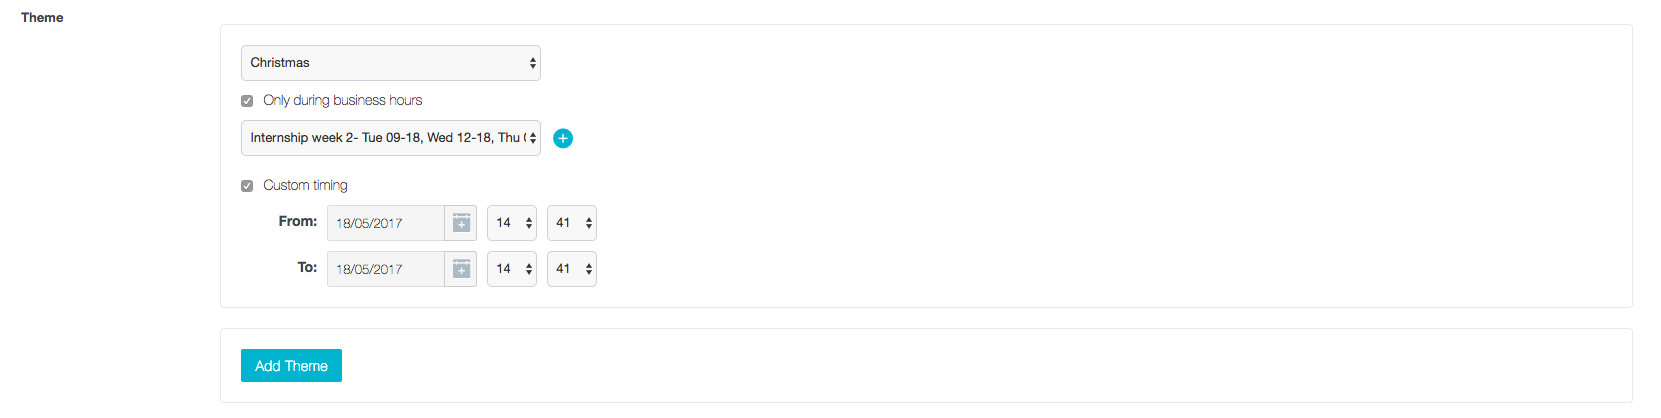
\includegraphics[width=1\textwidth]{Figuren/ThemeSet.png}
	\caption{Plannen van een thema}
	\label{fig:ThemeSet}
\end{figure}
%MSS TASK VERTALEN NAAR GWN TAAK??
Na het opstellen van een planning kan het profiel opgeslagen worden. Is dit een nieuw profiel, waar nog nooit iets voor werd ingesteld, dan wordt hiervoor een nieuwe \textit{task} aangemaakt. Een \textit{task} wordt gekenmerkt door een ID, een groep, een account, data, prioriteit, \texttt{nextScheduleDate} en \texttt{lastSuccessfulRun}. Aangezien \'{e}\'{e}n taak per profiel wordt aangemaakt, volstaat het om het profiel ID te gebruiken om de taken van elkaar te onderscheiden. De groep bepaald waartoe de taak behoort, hier dus de \texttt{profile-manager}. Als data wordt simpelweg het ID van het profiel gebruikt. De data bevat alles nodige informatie om de taak correct uit te voeren. Er wordt verwacht dat de \textit{task} onmiddellijk uitgevoerd wordt dus wordt als \texttt{nextScheduleDate} het huidige tijdstip genomen. 

Eens de taak aangemaakt is, wordt deze in de database opgeslagen en via de \textit{scheduler}, indien nodig, op de \textit{queue} geplaatst. Eens een taak in de \textit{queue} staat, wordt deze op zijn beurt uitgevoerd. Het uitvoeren van de taak gebeurt met behulp van de \textit{dispatcher}. Deze linkt de correcte \textit{handler} aan de taak zelf. In de \textit{handler} wordt de taak dan afgehandeld en wordt een volgende taak gepland. Het schema op Figuur \ref{fig:UniCrawler} toont het volledige proces. 

\begin{figure}[H]
	\centering
	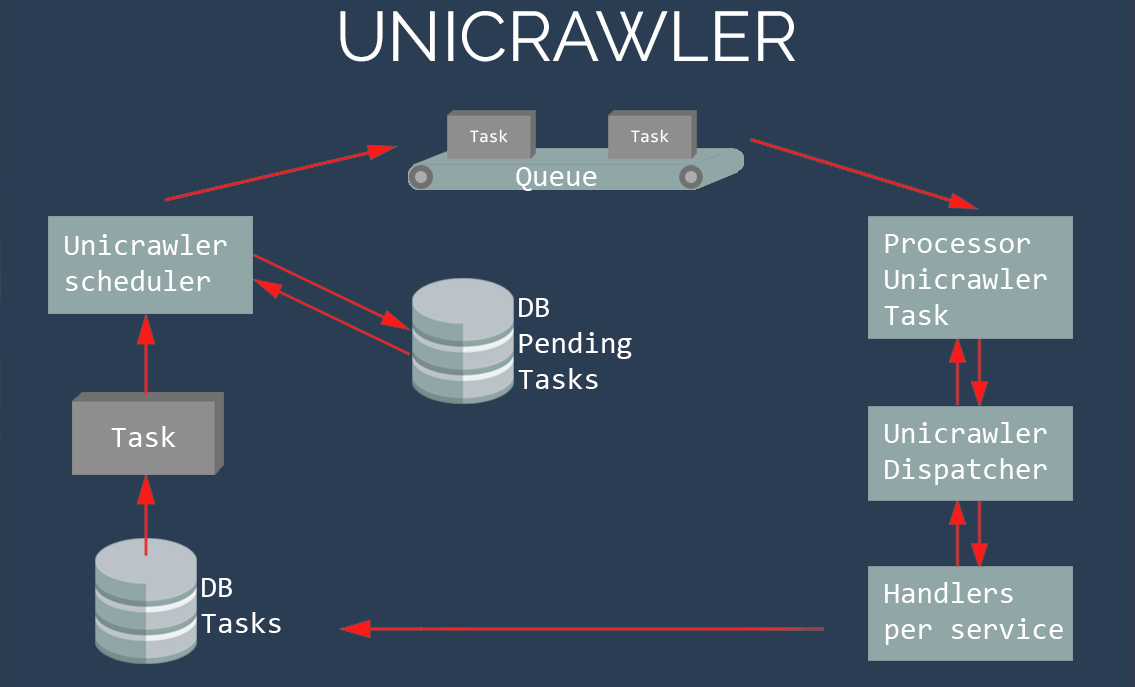
\includegraphics[width=1\textwidth]{Figuren/UniCrawler.png}
	\caption{UniCrawler}
	\label{fig:UniCrawler}
\end{figure}

Aangezien het de bedoeling is dat het thema op een profiel up-to-date gehouden wordt, wordt een taak om de vijf minuten herhaald. %REWRITE DIS SENTENCE <--
Bij het afhandelen van de taak worden verschillende checks uitgevoerd om te bepalen of het thema daadwerkelijk toegepast moet worden. Wanneer hetzelfde thema nog steeds actief is of de KPI's niet verandert zijn, is het nutteloos om de foto's opnieuw te genereren en te uploaden. Voor er overgegaan kan worden naar het toepassen van het thema, moet natuurlijk eerst bepaald worden welk thema actief moet zijn. 

Om dit te weten te komen, wordt gebruik gemaakt van een algoritme. Dit algoritme haalt voor een profiel alle ingeplande thema's op. Voor ieder thema wordt gekeken of deze een aangepaste \textit{timing} bevat of \textit{business hours} of beide. Valt het huidige tijdstip (waarop de taak dus wordt afgehandeld) binnen de ingestelde \textit{timing} dan wordt alle informatie over dat bepaalde thema bijgehouden. Hier moet vermeld worden dat tijdstippen uitgedrukt worden in Unix tijd om het vergelijken te vereenvoudigen. Eens de \textit{custom timing} bekeken is, worden alle ingestelde \textit{business hours schedules} overlopen. Gebruikers kunnen namelijk meerdere \textit{schedules} selecteren om zo de planning gedetailleerder te maken. De tijdstippen van deze \textit{schedules} worden vergeleken met het reeds berekende tijdstip en het meest recente wordt toegevoegd aan een lijst. Uit deze lijst wordt dan het meest recentste tijdstip genomen. Zo wordt het thema gevonden dat op dat moment actief moet zijn op basis van de \textit{business hours schedules}. Uiteindelijk wordt de berekende \textit{custom timing} vergeleken met de \textit{business hours} om te bepalen wat de bovenhand neemt. 

Wordt dit algoritme op iedere set (zie Figuur \ref{fig:ThemeSet}) toegepast, wordt uiteindelijk een lijst bekomen met het tijdstip van iedere set die op dat moment actief kan zijn. Met behulp van een sorteermethode worden alle sets aflopend geordend. De eerste in de lijst (met de hoogste waarde) is dan het actieve thema en moet dus ingesteld worden op het profiel. Wordt noch een \textit{custom timing} noch een \textit{business hours schedule} gevonden, dan wordt deze set eenvoudigweg aan dezelfde lijst toegevoegd met een timestamp die gelijk is aan 0. Het thema in deze set zal dus enkel actief zijn wanneer geen andere sets die aan de eisen voldoen, aanwezig zijn. Sets zonder enige specificaties kunnen dus als standaard thema voor een profiel ingesteld worden. 

%MAYBE DELETE?
Verschillende sets kunnen dus zo geconfigureerd worden dat een complexe planning van thema's ontstaat. Zo kunnen gebruikers bijvoorbeeld een standaard thema ingesteld hebben voor hun profiel maar wordt tijdens de openingsuren op de omslagfoto aangegeven dat het bedrijf open is. Op bepaalde feestdagen zoals Kerstmis of Pasen kan dan weer een aangepaste profielfoto getoond worden. 

\subsection{Doorsturen naar Facebook/Twitter - Uploaden naar sociale media}
Elke vijf minuten bestaat de kans dat een thema toegepast wordt en dus ook foto's ge\"{u}pload moeten worden naar Facebook of Twitter. Binnen CX Social wordt reeds gebruik gemaakt van de Application Programming Interface (API) van deze platformen waardoor er reeds code aanwezig is voor het maken van een \textit{request} naar elk van deze services. Deze code zal ook een correct authenticatie token, voor de ingelogde gebruiker, met de \textit{request} meegeven. %MSS WEGLATEN <-- ? MEER UITLEG EROVER!! OAUTH 2 ENZO!!
Er moet dus enkel een \textit{request} gestuurd worden naar de specifieke \textit{endpoints} waarmee profielfoto, omslagfoto en profielinformatie aangepast worden. 

\textbf{Twitter} \break
Om de omslagfoto van een Twitter-profiel aan te passen wordt gebruik gemaakt van de \texttt{/account/updateo{\_}profileo{\_}banner} \textit{endpoint} \cite{TwitterAPIDoc}. De afbeelding zelf kan base64 ge\"{e}ncodeerd of als \textit{raw image data} meegegeven worden. Aangezien de omslagfoto's telkens door de Node.js service worden gegenereerd en dus in het base64 formaat ontvangen worden (zie sectie \ref{ExporterenVanHetCanvas}), kand de afbeelding rechtstreeks meegegeven worden aan het \textit{endpoint}. Zoals te zien in codefragment \ref{lst:TwitterAPICall} worden de URL naar de \textit{endpoint}, de afbeelding, \textit{request} methode en enkele opties verwacht om de \textit{call} te maken. Een van de opties is het verwachte antwoord op de \textit{request}. Dit kunnen zowel een HTTP status codes 200 (OK), 201 (Created) of 202 (Accepted) zijn. 

\begin{lstlisting}[caption={Uploaden van omslagfoto naar Twitter},label=lst:TwitterAPICall,language=PHP]
try {
	$updateBanner = $this->call(
		self::API_VERSION . '/account/update_profile_banner',
		array(
			'banner' => $image
		),
		'POST',
    	/* $multipart = */ false,
		/* $options = */ array(
		'expectedResponseCodes' => array(200, 201, 202)
	)
);

} catch (Exception $ex) {
	throw $ex;
}
\end{lstlisting}

Het uploaden van de profielfoto verloopt op gelijkaardige manier. Via de \texttt{/account/updateo{\_}profileo{\_}image} \textit{endpoint} wordt de base64 ge\"{e}ncodeerde afbeelding naar Twitter gestuurd \cite{TwitterAPIDoc}. In tegenstelling tot de omslagfoto moet een profielfoto niet geannoteerd worden. Hierdoor kan de afbeelding simpelweg vanop de fileserver gehaald worden. Deze foto wordt dan base64 ge\"{e}ncodeerd voor gebruik op Twitter.

\textbf{Facebook} \break
De Graph API van Facebook biedt de mogelijkheid om omslag-en profielfoto aan te passen. Dit is echter een heel stuk complexer bij Facebook dan bij Twitter. %MSS REMOVE? <--
Facebook verwacht namelijk dat gebruikers een foto, die reeds op hun tijdlijn staat, zullen instellen als omslagfoto. Dit betekent dat een foto eerst ge\"{u}pload wordt naar Facebook waarna deze als omslagfoto of profielfoto wordt ingesteld. Dit zorgt ervoor dat de foto niet enkel in het album met tijdlijnfoto's maar ook in het album met omslagfoto's of profielfoto's terecht komt. Wordt aangenomen dat een foto om de vijf minuten ge\"{u}pload wordt, is al snel duidelijk dat de verschillende albums rond de 300 foto's zullen bevatten na \'{e}\'{e}n dag. 

Dit is natuurlijk niet de bedoeling dus wordt dit probleem op volgende manier opgelost. %ISDA JUIST??? <--

Met behulp van de \texttt{/page-id/photos} \textit{edge} wordt een foto naar Facebook ge\"{u}pload. Een foto naar een pagina uploaden kan op twee manieren: via een verwijzing naar een foto die reeds op het internet staat (dus via een URL) of de afbeelding toevoegen als \texttt{multipart/form-data}. Mits de gegenereerde foto's nog niet beschikbaar zijn op het internet, wordt voor de laatste methode geopteerd. Naast een \textit{access token} en wat opties, wordt het pad naar het bestand als \textit{source} parameter meegegeven. Aangezien het niet gewenst is om een notificatie te krijgen wanneer een omslag-of profielfoto wordt gewijzigd, wordt de \textit{no{\_}story} parameter ook actief gezet (zie codefragment \ref{lst:FacebookAPICallUpload}) \cite{FacebookPagePhotos}. 

\begin{lstlisting}[caption={Uploaden van een foto naar Facebook},label=lst:FacebookAPICallUpload,language=PHP]
$uploadedPhotoId = $this->call(
	'/' . Services_Facebook_Migrations::VERSION_2_8 . '/' . $this->getServiceId() . '/photos',
	$this->getAccessToken(),
	Services_Facebook_Manager::MODE_JSON,
	'POST',
	array(
		'source' => '@' . realpath($tempFile),
		'no_story' => true,
	),
	/* options */ array( 
		'postFieldsAsString' => false,
		'timeout' => static::UPLOAD_TIMEOUT,
	)
);
\end{lstlisting}

%ASK WHERE THE AUTH TOKEN COMES FROM! https://developers.facebook.com/tools/explorer?method=GET&path=me%2Faccounts&version=v2.9
%https://en.wikipedia.org/wiki/OAuth  https://www.youtube.com/watch?v=L1PDqJkedZ0

%Facebook -> Dit is zeker niet de beste oplossing maar momenteel de meest gebruiksvriendelijke. 
Na het uploaden van een foto naar de tijdlijn wordt als antwoord het ID van deze foto ontvangen. Met een call naar de pagina zelf kan deze foto ingesteld worden als omslagfoto. Parameters hierbij zijn \textit{cover} (het ID van de foto) en \textit{offset{\_}x} en \textit{offset{\_}y} van de omslagfoto (zie codefragment \ref{lst:FacebookAPICallCover}). Ook hier wordt de \textit{no{\_}feed{\_}story} parameter toegevoegd om te vermijden dat volgers van de pagina, om de x aantal minuten, een notificatie ontvangen. 

Uiteindelijk worden enkele maatregelen getroffen om het aantal foto's in de albums te beperken. Zo wordt v\'{o}\'{o}r het uploaden van een nieuwe foto, het ID van de huidige afbeelding opgehaald. Na het instellen van de nieuwe afbeelding, kan de andere foto via het ID uit het album verwijdert worden. Uiteindelijk wordt de foto ook uit het tijdlijn album verwijdert. Op deze manier wordt het aantal foto's in de albums tot een minimum beperkt.

\begin{lstlisting}[caption={Instellen van omslagfoto op Facebook},label=lst:FacebookAPICallCover,language=PHP]
$coverPhoto = $this->call(
	'/' . Services_Facebook_Migrations::VERSION_2_8 . '/' . $this->getServiceId(),
	$this->getAccessToken(),
	Services_Facebook_Manager::MODE_JSON,
	'POST',
	array(
		'cover' => $uploadedPhotoId['id'],
		'offset_x' => 0,
		'offset_y' => 0,
		'no_feed_story' => true
	),
	array(
		'timeout' => static::UPLOAD_TIMEOUT,
	)
);
\end{lstlisting}

Het uploaden van een profielfoto verloopt op gelijkaardige manier. Het instellen als avatar gebeurt hier via de \texttt{/page-id/picture} edge van de Graph API \cite{FacebookPagePicture}. Als parameters worden \textit{photo} (het ID van de foto in het tijdlijn album), \textit{width}, \textit{height} en \textit{no{\_}feed{\_}story} meegegeven. De hoogte en breedte van de foto worden ingesteld op 200 pixesl omdat Facebook een foto van minimum 180 op 180 pixels verwacht \cite{FacebookDimensions}. 

Net zoals bij het instellen van een omslagfoto moeten de vorige profielfoto en de ge\"{u}ploade foto verwijdert worden om een overvloed aan foto's te vermijden. In tegenstelling tot de omslagfoto, kan het ID van de huidige profielfoto niet opgehaald worden. Wanneer het ID niet beschikbaar is, kan ook de correcte foto niet verwijdert worden. Om dit probleem op te lossen wordt het volledige album van profielfoto's opgehaald. Aangezien de eerste foto in dit album de huidige profielfoto is, kan het ID hier uit gehaald worden om zo de foto te verwijderen. Hoewel deze methode het ene probleem oplost, veroorzaakt het een ander. Het verwijderen van de eerste foto in het album zorgt er voor dat gebruikers zelf geen profielfoto kunnen instellen via Facebook zelf. Deze zal namelijk verwijdert worden wanneer een thema wordt toegepast. De kans dat dit voorkomt is echter miniem omdat verwacht wordt van gebruikers dat ze de foto aanpassen vanuit de Profile Manager en niet op het profiel zelf. 

\iffalse
\subsection{Afbeeldingcompressie?}
Bij het uitwerken van dit project werd ook even stilgestaan bij afbeeldingcompressie. Het is namelijk niet gewenst om zeer grote afbeeldingen in te laden en/of op te slaan. Gelukkig kunnen heel wat problemen vermeden worden bij dit project. Een foto moet slechts op \'{e}\'{e}n plaats daadwerkelijk opgeslagen worden. Wanneer de gebruiker een nieuw thema aanmaakt, kunnen een omslagfoto en avatar gekozen worden. Bij het selecteren van de foto wordt deze naar de fileserver ge\"{u}pload. Ook hier wordt geen compressie toegepast maar er wordt gezorgd dat de bestanden niet groter zijn dan 3 megabyte. 

Waar op andere plaatsen in het project gebruik gemaakt wordt van foto's, wordt telkens met de base64 ge\"{e}ncodeerde foto gewerkt. Dit betekent dat de foto simpelweg als tekst verstuurd kan worden. Deze foto's worden opgebouwd met onder andere het bestand dat reeds op de fileserver staat. 
\fi


 %telkens de link naar het ge\"{u}ploade bestand gebruikt. 

\chapter{Algemeen besluit}
\vspace{-3cm}

%\iffalse
%Zowel tijdens het uitwerken van de stageopdracht als tijdens het schrijven van deze bachelorproef werd heel wat bijgeleerd. Met de nieuw verworven kennis werd het implementeren van een Profile Manager binnen de CX Social webapplicatie mogelijk. De kern van deze feature was het dynamisch annoteren van afbeeldingen. 
Tijdens het uitwerken van deze bachelorproef werd kennis gemaakt met heel wat nieuwe technologie\"{e}n. Met de nieuw verworven kennis werd het implementeren van een Profile Manager binnen de CX Social applicatie mogelijk. Naast het werken met bibliotheken zoals Fabric.js werd 

Aangezien de Profile Manager een redelijk uitgebreide feature is, werden heel wat doelstellingen gesteld. Naast het uitwerken van een data model en het schrijven van de nodige testen, waren het annoteren van de afbeeldingen en deze periodiek uploaden naar sociale media het belangrijkst. Het implementeren van dit alles werd gespreidt over de volledige periode dat stage gelopen werd. Hoewel deze feature zeer uitgebreid is en heel wat functionaliteit bevat, werden de meeste doelstellingen behaald. Zeker de belangrijkste elementen zijn volledige uitgewerkt. Onderzoek naar een bibliotheek die het manipuleren van afbeeldingen vereenvoudigen was noodzakelijk aangezien dit de kern was van de stageopdracht. Na onderzoek bleek Fabric.js de perfecte bibliotheek te zijn en kon de nodige functionaliteit ge\"{i}mplementeerd worden.
% Dit houdt in dat gebruikers een thema kunnen aanmaken en dit later in te stellen voor \'{e}\'{e}n of meerdere profielen. Een thema kan een zowel een omslagfoto en profielfoto bevatten en aan de omslagfoto kunnen annotaties toegevoegd worden. Annotaties kunnen zowel tekst als dynamische KPI's zijn waardoor gebruikers hun omslagfoto zeer uitgebreid kunnen personaliseren.

De Profile Manager kan voor veel bedrijven en ondernemingen een meerwaarde zijn voor hun sociale media management. Vooral het feit dat de KPI's up-to-date gehouden worden, maakt het mogelijk om hun klanten vitale informatie te bezorgen. Doordat thema's ingesteld kunnen worden om actief te zijn op verschillende tijdstippen wordt heel wat werk bespaard. 

Door het functioneren in een team, werden heel wat nieuwe inzichten verworven. Rekening houdend met visies en expertise van teamgenoten, wordt het mogelijk om problemen op een totaal andere manier aan te pakken. Naast een \textit{second opinion} over reeds geschreven code, kon ook om hulp gevraagd worden tijdens het aanpakken van venijnige problemen. Wanneer een hardnekking probleem niet opgelost kon worden na zelfstandig onderzoek kon altijd hulp ingeroepen worden. Ook door de mogelijkheid tot persoonlijke inbreng, werd het werken in een team zeer aangenaam. 

Wekelijkse meetings droegen bij tot het effici\"{e}nt en correct uitwerken van de annotatie feature binnen de Profile Manager. In samenwerking met de designer werden zowel veranderingen in het ontwerp als in de functionaliteit uitgevoerd om kleine beperkingen van de bibliotheek te omzeilen. Ook dit zorgde voor een andere kijk op de implementatie aangezien niet enkel naar de code maar ook naar het ontwerp en uiteindelijk de gebruikservaring werd gekeken. 

Na 12 weken intensief werken aan de Profile Manager, kon de beta versie online geplaatst worden. Deze versie zal uitgebreid getest worden door het support team en wanneer geen problemen meer gevonden worden, kan de feature online geplaatst worden. Eens beschikbaar, zal het zeker een meerwaarde vormen voor verschillende klanten. Het feit dat deze feature actief gebruikt zal worden door bedrijven is een directe beloning voor het verrichte werk.  

















%// Zeer handige feature
%// Mogelijkheid tot persoonlijke inbreng. Vooral bij de kleinere functionaliteiten en hoe zaken geimplementeerd moeten worden
%// De meeste doelstellingen zijn bereikt van het opgestelde actieplan. Enkel de integratie in de crisisplans (en welcome messages) zijn er niet 
%\fi
%\include{Conclusies}

%\backmatter

\bibliographystyle{ieeetr}
\mainmatter
\addcontentsline{toc}{chapter}{Bibliografie}


\bibliography{Bibliografie}


\appendix
\chapter{Bijlage}
\iffalse
\section{Naive Bayes op basis van ingredi\"{e}nten }
\begin{lstlisting}
# inladen van de data
ReceptenJO.binair <- read.table("ReceptenJO.binair.csv", 
	header=TRUE, quote="\"")

# SPLITSEN VAN DE DATASET IN TEST EN TRAIN DATA
nfolds <- 4

id <- rep(1: nfolds,length.out=dim(ReceptenJO.binair)[1])
id <- sample(id,dim(ReceptenJO.binair)[1])
id.test <- (1:dim(ReceptenJO.binair)[1])[id==1]
id.train <- (1:dim(ReceptenJO.binair)[1])[id!=1]

Recepten.test <- ReceptenJO.binair[id.test,]
Recepten.train <- ReceptenJO.binair[id.train,] 

Bernoulli_NB <- function(ReceptenJO.train, ingredienten){
# SCHRIJVEN VAN NAIVE BAYES MODEL OBV INGREDIENTEN
# De input is een binaire vector 
# die de aan- & afwezigheid van ingredienten weergeeft
# De output is het keukentype waarin het recept geclassificeerd werd
  
# kans dat een ingredient in een gegeven keuken voorkomt
# pseudocounts = 0.01
Recepten.train[1:372] <- as.matrix(Recepten.train[1:372]) + 0.01 
IngredientenJO <- Recepten.train[,1:373] 
likelihoodIngred <-aggregate(.~cuisine, IngredientenJO, mean)
likelihoodIngred$cuisine <- NULL

# enkel de ingredienten nodig als input, niet het keukentype
# en de nutritionele waarden: 
# kolom 1 tem 372 wordt dus geselecteerd
input <- as.matrix(ingredienten[1:372]) 

# initialisatie: er zijn 10 keukentypes met 372 ingredienten    
likelihood <- matrix(0,10,372) 
  for (j in 1:10){
    for (k in 1:372){
      likelihood[j,k] = input[k]* likelihoodIngred[j,k] + 
												(1-input[k])*(1-likelihoodIngred[j,k])
    }
  }
	
# matrix met dimensies 10x372
loglikelihood <- log(likelihood)
# wanneer likelihood = 1, is de loglikelihood = 0
# DUS corrigeren met pseudocounts 0.01 => log(0.99) ipv log(1)
loglikelihood[is.na(loglikelihood)] <- log(0.99) 
# loglikelihood geeft nu per keukentype de kans dat de ingegeven
# ingredientenCOMBINATIE (input) in die bepaalde keuken voorkomt 
# DUS matrix met dimensies 10x1
  
loglikelihood <- apply(loglikelihood,1,sum) 

keukentypes <- levels(Recepten.train$cuisine)
maximum <- max(loglikelihood)
index <- loglikelihood==maximum
keukentype <- keukentypes[index]
  
  return(keukentype)
}


# TESTEN OP TESTDATA + CONFUSIONMATRIX OPSTELLEN
voorspelling <- matrix(0,length(Recepten.test[,1]), 1)

for (i in 1 : length(Recepten.test[,1])){
  voorspelling[i] <-Bernoulli_NB(Recepten.train,Recepten.test[i,])
}

confusionTable <- table(voorspelling, as.matrix(Recepten.test$cuisine))

\end{lstlisting}
\fi

\end{document}